
%%%%%%%%%%%%%%%%%%%%%%%%%%%%%%%%%%%%%%%%%%%%%%%%%%%%%%%%%%%%%%%%%
%  _____   ____  _____                                          %
% |_   _| /  __||  __ \    Institute of Computitional Physics   %
%   | |  |  /   | |__) |   Zuercher Hochschule Winterthur       %
%   | |  | (    |  ___/    (University of Applied Sciences)     %
%  _| |_ |  \__ | |        8401 Winterthur, Switzerland         %
% |_____| \____||_|                                             %
%%%%%%%%%%%%%%%%%%%%%%%%%%%%%%%%%%%%%%%%%%%%%%%%%%%%%%%%%%%%%%%%%
%
% Project     : LaTeX doc Vorlage für Windows ProTeXt mit TexMakerX
% Title       : 
% File        : vorgehen.tex Rev. 00
% Date        : 7.5.12
% Author      : Remo Ritzmann
% Feedback bitte an Email: remo.ritzmann@pfunzle.ch
%
%%%%%%%%%%%%%%%%%%%%%%%%%%%%%%%%%%%%%%%%%%%%%%%%%%%%%%%%%%%%%%%%%

\chapter{Approach and Methodology}\label{chap.vorgehen}
\section{Work Approach}\label{basic_cons}
As described under \autoref{baseline}, our work is based on the work of S. Huschauer \cite{flatlandstephan}. We take the idea of using the A3C algorithm to solve the Flatland problem and try various modifications in an attempt to improve its performance. We proceed by giving an idea, what we want to achieve by changing the specified part, followed by an experiment to either prove or disprove our hypothesis. We do this in an iterative manner, to gradually come closer to a well-performing solution for Flatland.\\
In our experiments, we focus exclusively on Flatland round 2. While we compare our solution for round 1 in \autoref{chap.resultate}, all technical improvements are also part of our solution for round 2.\\
Our work can be categorized into a section about reinforcement learning for Flatland (\autoref{rl_flatland}) and a section about infrastructure and scaling up the training process (\autoref{dist_architecture}).\\
\section{Reproducability in Reinforcement Learning}\label{reproducability}
It is important to note, that the training process of reinforcement learning and especially multi agent reinforcement learning can be hard to reproduce. Depending on the initial weights of the neural networks and the layout of the environments, the performance may vary on each restart. Also in a distributed algorithm, the number of workers can significantly influence the training performance. If not differently specified, we execute all presented experiments on machines with the same specifications (see \autoref{infrastructure}).\\
Another aspect that is hard to reproduce is training stability. In A3C, an important instrument to prevent the policy from converging too early is using an additional entropy term \cite{a3c}. Our way to maintain stability with changing environments is discussed in \autoref{entropy_balancing_hyperparameter}.\\
For better comparability, we try to keep our experimental versions of the training as similar to each other as possible. If not differently specified, we run evaluations with the following setup:
\begin{itemize}
	\item We use an environment of the size 100x100 tiles with 14 individual agents.
	\item The map contains 20 cities
	\item There is a maximum of 3 rails between cities and a maximum of 4 rails inside cities
	\item Based on the flatland specification, the maximum allowed number of timesteps is 1608 \cite{flatland_spec}.
\end{itemize}
To analyze the performance of the solution, we run an analyzer that executes 20 rollouts of the environment using the same neural network parameters. After the these 20 rollouts, we update the neural network parameters. For each evaluation round, we use the same 20 environment layouts. 
To compare the performance in a graph, we now take the mean number of agents arrived at their target and plot that in our graph.
\chapter{Experiment Design and Analysis}\label{chap.experiment}
\section{Reinforcement Learning for Flatland}\label{rl_flatland}
\subsection*{A3C Implementation}\label{a3c_implementation}
Originally, the asynchronous advantage actor critic algorithm (A3C) has been designed for use in a single agent environment \cite{a3c}.
By applying it in a multi agent environment, we implicitly convert the environment into a non-stationary system.
While applying A3C in a multi agent setting, the other agents can be viewed as part of the environment. This means, the behaviour of the environment changes while training, due to the fact that the behaviour of the other agents changes.
Gupta et al.finds in \cite{multiagent_comp_a3c_dqn_etc}, that RL methods like Deep-Q networks (DQN) and Trust region policy optimization (TRPO) are not performing well in a multi agent environment, due to the combination of experience replay and non-stationarity of the environment. We therefore suggest, that it is not recommendable to keep an experience replay buffer with older episodes. Otherwise the sampled experience might represent old agent behaviour which is then learned to deal with.\\
An important implementation detail in our version is, that we do not perform updates during episodes but only at their end. The reason for this is, that the only possibility for an agent to receive reward is at the end of the episode. Therefore would any earlier update have a reward of 0 and not help the training process.
\subsection*{Observation Design}\label{enhanced_observations}
The Flatland environment provides a base to build custom observation builders that can be used to create a state representation for the agents as explained in \autoref{observations}. In this work, we do not consider the usage of the grid-based observation builders.
Both the Flatland development team as well as S. Huschauer find, that tree based observations work better in their experiments \cite{flatlandstephan}. The Flatland specification states \cite{flatland_spec}:
\begin{quote}
Considering, that the actions and directions an agent can chose in any given cell, it becomes clear that a grid like observation around an agent will not contain much useful information, as most of the observed cells are not reachable nor play a significant role in for the agents decisions.
\end{quote}
Based on the provided TreeObsForRailEnv (see \autoref{observations}), we implement a custom observation builder which we use to produce an input vector for our neural network. This observation builder takes the the current state of the environment and produces a fixed size numeric vector with values between 0.0 and 1.0 for each agent. This input vector should fulfil an number of requirements:
\begin{itemize}
	\item Each rail section the agent possibly rides on next should be visible to the agent.
	\item The agent should be able to detect, whether there is another train coming the opposite direction on any section.
	\item The agent should be able to detect on each switch which turn is the faster way to his target.
	\item On switches, the agent should be able to see if a turn does lead to his target, even if it is not the fastest way. If this is the case, taking this turn might even be a good option to evade possibly blocking situations.
	\item For the next grid tile, the agent should be able to detect if it is a switch and if so, if it is one the agent can make a decision on. (see \autoref{flatland_intro} for non-usable switches).
\end{itemize}
The provided TreeObsForRailEnv produce a graph with a node for each section of the rail. We extend these nodes with additional information about train traffic coming the other direction than the one the agent is heading. We take the information from these nodes and convert them into a numeric vector. In case that there is a dead end, we fill the observation with zeros (this could only happen in Flatland round 1, round 2 does not have dead ends). After the conversion, we concatenate all section observations into one large vector with information for all upcoming sections.\\
While this vector already contains all required information outside of the agent, we add another vector with information regarding the agent itself (train specific observation in \autoref{obs_descr}). This vector contains the speed of the agent, the max. speed of the agent, the type of the current tile, the direction the agent is heading and 
\begin{figure}
	\centering
	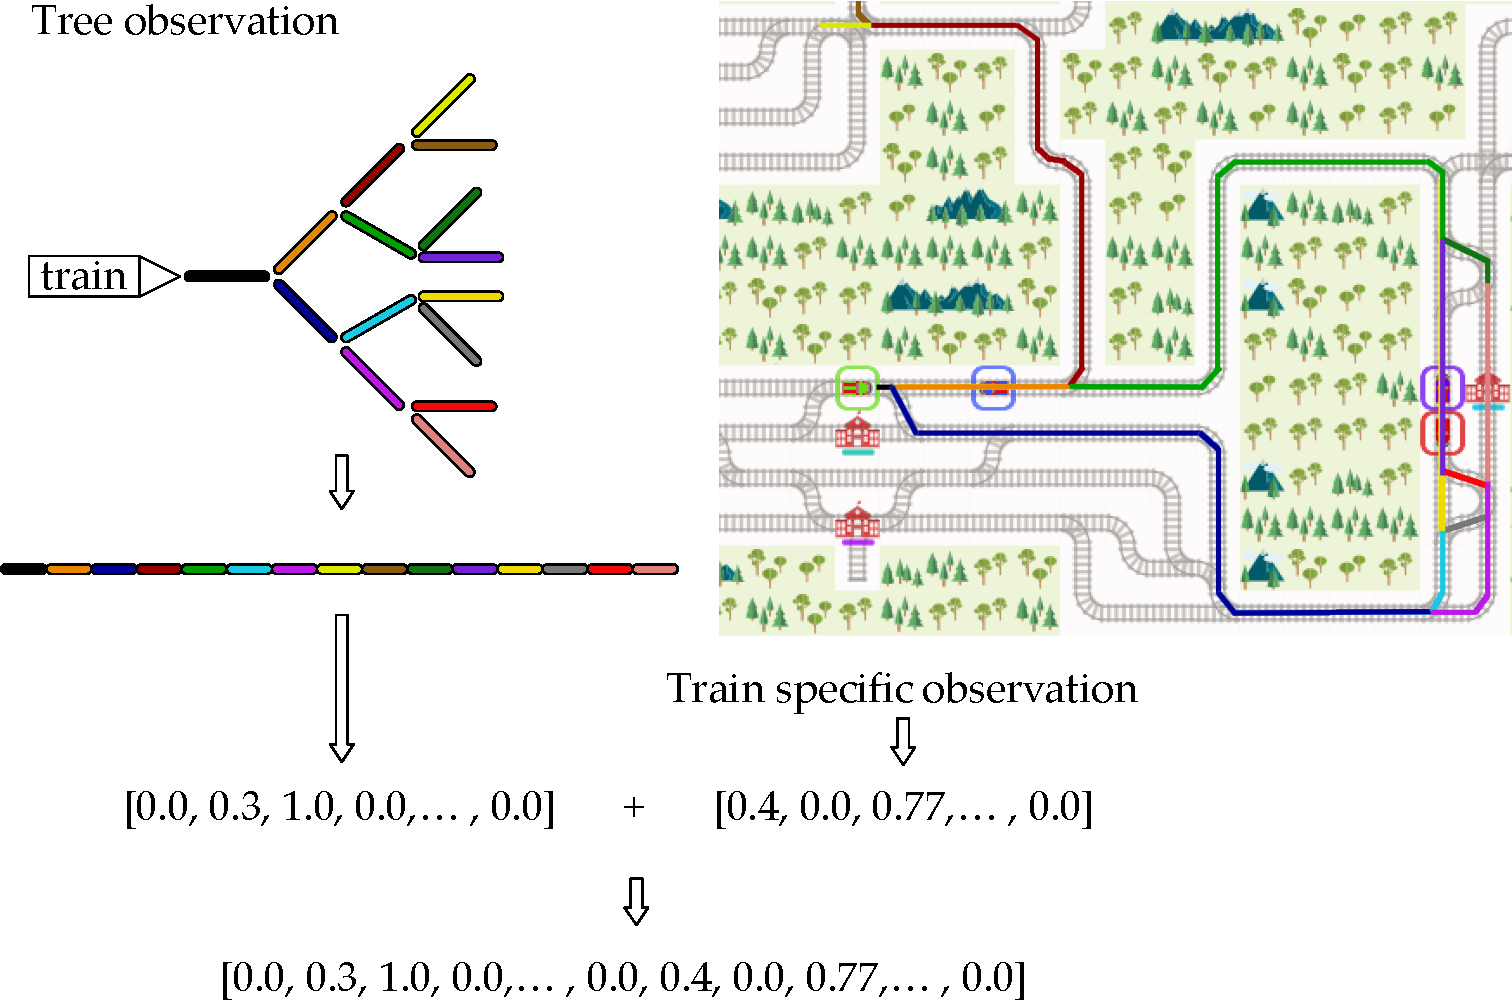
\includegraphics[width=300pt]{diagrams/tree_obs_mapping.pdf}
	\caption{Illustration of the tree observation mapped onto the Flatland enviornment. Each colored bar represents information about a section.}
	\label{obs_descr}
\end{figure}
\subsection*{Action Space Reduction and Script Policy Actions}\label{reduced_action_space}
The Flatland environment is designed in a way to resemble a classical RL environment. This means, on every timestep, we receive observations for each agent, calculate an action and hand this action to the environment, visible in pseudocode \autoref{alg:no_reduction}.\\\\
\begin{algorithm}[H]
	\KwData{initialized Flatland environment $\mathcal{E}$, initial observation $\mathcal{s\SPSB{a}{t=0}}$ for all agents }
	\KwResult{terminal Flatland environment}
	initialize buffer $\mathcal{B}$\\
	\While{episode not terminal}{
		create empty action array $\mathcal{A}$\\
		\For{every agent $\mathcal{a}$}{
			get current state $\mathcal{s\SPSB{a}{t}}$ of agent\\
			// Fetch action for agent, based on current state\\
			$\mathcal{A[a]} \leftarrow$ from policy $\pi (\mathcal{s\SPSB{a}{t}})$\\
		}
		
		call $\mathcal{env.step(A)}$ \\
		retrieve reward $\mathcal{R}$\\
		append $\mathcal{A}$ to buffer $\mathcal{B}$\\
		retrieve all new states $\mathcal{s_{t+1}}$\\		
	}

	use buffer $\mathcal{B}$ for training of policy $\pi$
	\caption{Default episode for Flatland environment}
	\label{alg:no_reduction}
\end{algorithm}
While this makes sense in an environment where agents need to take an action on every timestep (such as Atari games), in Flatland most of the time the only reasonable action is to move forward as visible in \autoref{fig:no_desicion}. Only around switches, the actions of an agent have acutual consequences.
\begin{figure}[H]
	\centering
	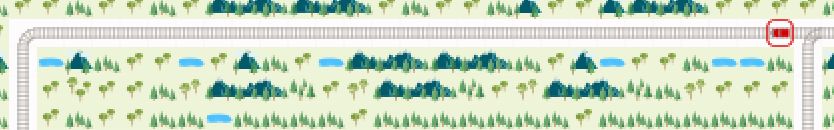
\includegraphics[width=300pt]{images/screenshot_no_decision.png}
	\caption{Screenshot from Flatland environment. A train heading east. The only reasonable action is to ride forward.}
	\label{fig:no_desicion}
\end{figure}
Every action that is produced by the neural network should be included for training, so the network can adapt to this type of situation. The problem arises now, that all these actions of riding forward are included into the training of the agent. The influence of the actions that actually matter (e.g. the ones around switches) is thereby not as big as it could be, because a large portion of the training data is actually situations that do not actually require decisions.\\
To solve this problem, we implement hard coded rules that the agents follow as long as they are not in a situation to make a decision. Only around switches, the neural network policy is activated. As a consequence, the data used for training has less samples but the samples available are of higher quality. The training with this mechanism implemented looks like \autoref{alg:with_reduction}.
For training, we only use the experience collected near the switch.\\
\begin{algorithm}[H]
	\KwData{initialized Flatland environment $\mathcal{env}$, initial observation $\mathcal{s\SPSB{a}{t=0}}$ for all agents}
	\KwResult{terminal Flatland environment}
	initialize buffer $\mathcal{B}$\\
	\While{episode not terminal}{
		create empty action array $\mathcal{A}$\\
		\For{every agent $\mathcal{a}$}{
			\eIf{agent is near to a switch}{
				get current state $\mathcal{s\SPSB{a}{t}}$ of agent\\
				// Fetch action for agent, based on current state\\
				$\mathcal{A[a]} \leftarrow$ from policy $\pi (\mathcal{s\SPSB{a}{t}})$\\
			}{
				$\mathcal{A[a]} \leftarrow \mathcal{u_{forward})}$
			}
		}
		call $\mathcal{env.step(A)}$ \\
		retrieve reward $\mathcal{R}$\\
		\If{agent was near switch}{
			append $\mathcal{s_{t}}$, $\mathcal{A}$ and $\mathcal{R}$ to buffer $\mathcal{B}$\\
		}
		retrieve all new states $\mathcal{s_{t+1}}$\\		
	}
	use buffer $\mathcal{B}$ for training of policy $\pi$

	\caption{Improved learning for flatland environment}
	\label{alg:with_reduction}
\end{algorithm}
This drastically improves training performance as visible in \autoref{chart:action_reduction_comparison}. While both versions have the potential to perform well, based on the observation data, we observe that the version without the action reduction is not able to performe nearly as well as the improved version with reduced actions.
\begin{figure}[H]
	\begin{center}
		%% Creator: Matplotlib, PGF backend
%%
%% To include the figure in your LaTeX document, write
%%   \input{<filename>.pgf}
%%
%% Make sure the required packages are loaded in your preamble
%%   \usepackage{pgf}
%%
%% Figures using additional raster images can only be included by \input if
%% they are in the same directory as the main LaTeX file. For loading figures
%% from other directories you can use the `import` package
%%   \usepackage{import}
%% and then include the figures with
%%   \import{<path to file>}{<filename>.pgf}
%%
%% Matplotlib used the following preamble
%%   \usepackage{fontspec}
%%
\begingroup%
\makeatletter%
\begin{pgfpicture}%
\pgfpathrectangle{\pgfpointorigin}{\pgfqpoint{5.000000in}{3.000000in}}%
\pgfusepath{use as bounding box, clip}%
\begin{pgfscope}%
\pgfsetbuttcap%
\pgfsetmiterjoin%
\definecolor{currentfill}{rgb}{1.000000,1.000000,1.000000}%
\pgfsetfillcolor{currentfill}%
\pgfsetlinewidth{0.000000pt}%
\definecolor{currentstroke}{rgb}{1.000000,1.000000,1.000000}%
\pgfsetstrokecolor{currentstroke}%
\pgfsetdash{}{0pt}%
\pgfpathmoveto{\pgfqpoint{0.000000in}{0.000000in}}%
\pgfpathlineto{\pgfqpoint{5.000000in}{0.000000in}}%
\pgfpathlineto{\pgfqpoint{5.000000in}{3.000000in}}%
\pgfpathlineto{\pgfqpoint{0.000000in}{3.000000in}}%
\pgfpathclose%
\pgfusepath{fill}%
\end{pgfscope}%
\begin{pgfscope}%
\pgfsetbuttcap%
\pgfsetmiterjoin%
\definecolor{currentfill}{rgb}{1.000000,1.000000,1.000000}%
\pgfsetfillcolor{currentfill}%
\pgfsetlinewidth{0.000000pt}%
\definecolor{currentstroke}{rgb}{0.000000,0.000000,0.000000}%
\pgfsetstrokecolor{currentstroke}%
\pgfsetstrokeopacity{0.000000}%
\pgfsetdash{}{0pt}%
\pgfpathmoveto{\pgfqpoint{0.606775in}{0.732921in}}%
\pgfpathlineto{\pgfqpoint{4.850000in}{0.732921in}}%
\pgfpathlineto{\pgfqpoint{4.850000in}{2.850000in}}%
\pgfpathlineto{\pgfqpoint{0.606775in}{2.850000in}}%
\pgfpathclose%
\pgfusepath{fill}%
\end{pgfscope}%
\begin{pgfscope}%
\pgfsetbuttcap%
\pgfsetroundjoin%
\definecolor{currentfill}{rgb}{0.000000,0.000000,0.000000}%
\pgfsetfillcolor{currentfill}%
\pgfsetlinewidth{0.803000pt}%
\definecolor{currentstroke}{rgb}{0.000000,0.000000,0.000000}%
\pgfsetstrokecolor{currentstroke}%
\pgfsetdash{}{0pt}%
\pgfsys@defobject{currentmarker}{\pgfqpoint{0.000000in}{-0.048611in}}{\pgfqpoint{0.000000in}{0.000000in}}{%
\pgfpathmoveto{\pgfqpoint{0.000000in}{0.000000in}}%
\pgfpathlineto{\pgfqpoint{0.000000in}{-0.048611in}}%
\pgfusepath{stroke,fill}%
}%
\begin{pgfscope}%
\pgfsys@transformshift{0.799649in}{0.732921in}%
\pgfsys@useobject{currentmarker}{}%
\end{pgfscope}%
\end{pgfscope}%
\begin{pgfscope}%
\definecolor{textcolor}{rgb}{0.000000,0.000000,0.000000}%
\pgfsetstrokecolor{textcolor}%
\pgfsetfillcolor{textcolor}%
\pgftext[x=0.445299in,y=0.355418in,left,base,rotate=30.000000]{\color{textcolor}\rmfamily\fontsize{10.000000}{12.000000}\selectfont 00:00h}%
\end{pgfscope}%
\begin{pgfscope}%
\pgfsetbuttcap%
\pgfsetroundjoin%
\definecolor{currentfill}{rgb}{0.000000,0.000000,0.000000}%
\pgfsetfillcolor{currentfill}%
\pgfsetlinewidth{0.803000pt}%
\definecolor{currentstroke}{rgb}{0.000000,0.000000,0.000000}%
\pgfsetstrokecolor{currentstroke}%
\pgfsetdash{}{0pt}%
\pgfsys@defobject{currentmarker}{\pgfqpoint{0.000000in}{-0.048611in}}{\pgfqpoint{0.000000in}{0.000000in}}{%
\pgfpathmoveto{\pgfqpoint{0.000000in}{0.000000in}}%
\pgfpathlineto{\pgfqpoint{0.000000in}{-0.048611in}}%
\pgfusepath{stroke,fill}%
}%
\begin{pgfscope}%
\pgfsys@transformshift{1.443023in}{0.732921in}%
\pgfsys@useobject{currentmarker}{}%
\end{pgfscope}%
\end{pgfscope}%
\begin{pgfscope}%
\definecolor{textcolor}{rgb}{0.000000,0.000000,0.000000}%
\pgfsetstrokecolor{textcolor}%
\pgfsetfillcolor{textcolor}%
\pgftext[x=1.088674in,y=0.355418in,left,base,rotate=30.000000]{\color{textcolor}\rmfamily\fontsize{10.000000}{12.000000}\selectfont 02:00h}%
\end{pgfscope}%
\begin{pgfscope}%
\pgfsetbuttcap%
\pgfsetroundjoin%
\definecolor{currentfill}{rgb}{0.000000,0.000000,0.000000}%
\pgfsetfillcolor{currentfill}%
\pgfsetlinewidth{0.803000pt}%
\definecolor{currentstroke}{rgb}{0.000000,0.000000,0.000000}%
\pgfsetstrokecolor{currentstroke}%
\pgfsetdash{}{0pt}%
\pgfsys@defobject{currentmarker}{\pgfqpoint{0.000000in}{-0.048611in}}{\pgfqpoint{0.000000in}{0.000000in}}{%
\pgfpathmoveto{\pgfqpoint{0.000000in}{0.000000in}}%
\pgfpathlineto{\pgfqpoint{0.000000in}{-0.048611in}}%
\pgfusepath{stroke,fill}%
}%
\begin{pgfscope}%
\pgfsys@transformshift{2.086398in}{0.732921in}%
\pgfsys@useobject{currentmarker}{}%
\end{pgfscope}%
\end{pgfscope}%
\begin{pgfscope}%
\definecolor{textcolor}{rgb}{0.000000,0.000000,0.000000}%
\pgfsetstrokecolor{textcolor}%
\pgfsetfillcolor{textcolor}%
\pgftext[x=1.732048in,y=0.355418in,left,base,rotate=30.000000]{\color{textcolor}\rmfamily\fontsize{10.000000}{12.000000}\selectfont 04:00h}%
\end{pgfscope}%
\begin{pgfscope}%
\pgfsetbuttcap%
\pgfsetroundjoin%
\definecolor{currentfill}{rgb}{0.000000,0.000000,0.000000}%
\pgfsetfillcolor{currentfill}%
\pgfsetlinewidth{0.803000pt}%
\definecolor{currentstroke}{rgb}{0.000000,0.000000,0.000000}%
\pgfsetstrokecolor{currentstroke}%
\pgfsetdash{}{0pt}%
\pgfsys@defobject{currentmarker}{\pgfqpoint{0.000000in}{-0.048611in}}{\pgfqpoint{0.000000in}{0.000000in}}{%
\pgfpathmoveto{\pgfqpoint{0.000000in}{0.000000in}}%
\pgfpathlineto{\pgfqpoint{0.000000in}{-0.048611in}}%
\pgfusepath{stroke,fill}%
}%
\begin{pgfscope}%
\pgfsys@transformshift{2.729772in}{0.732921in}%
\pgfsys@useobject{currentmarker}{}%
\end{pgfscope}%
\end{pgfscope}%
\begin{pgfscope}%
\definecolor{textcolor}{rgb}{0.000000,0.000000,0.000000}%
\pgfsetstrokecolor{textcolor}%
\pgfsetfillcolor{textcolor}%
\pgftext[x=2.375423in,y=0.355418in,left,base,rotate=30.000000]{\color{textcolor}\rmfamily\fontsize{10.000000}{12.000000}\selectfont 06:00h}%
\end{pgfscope}%
\begin{pgfscope}%
\pgfsetbuttcap%
\pgfsetroundjoin%
\definecolor{currentfill}{rgb}{0.000000,0.000000,0.000000}%
\pgfsetfillcolor{currentfill}%
\pgfsetlinewidth{0.803000pt}%
\definecolor{currentstroke}{rgb}{0.000000,0.000000,0.000000}%
\pgfsetstrokecolor{currentstroke}%
\pgfsetdash{}{0pt}%
\pgfsys@defobject{currentmarker}{\pgfqpoint{0.000000in}{-0.048611in}}{\pgfqpoint{0.000000in}{0.000000in}}{%
\pgfpathmoveto{\pgfqpoint{0.000000in}{0.000000in}}%
\pgfpathlineto{\pgfqpoint{0.000000in}{-0.048611in}}%
\pgfusepath{stroke,fill}%
}%
\begin{pgfscope}%
\pgfsys@transformshift{3.373147in}{0.732921in}%
\pgfsys@useobject{currentmarker}{}%
\end{pgfscope}%
\end{pgfscope}%
\begin{pgfscope}%
\definecolor{textcolor}{rgb}{0.000000,0.000000,0.000000}%
\pgfsetstrokecolor{textcolor}%
\pgfsetfillcolor{textcolor}%
\pgftext[x=3.018797in,y=0.355418in,left,base,rotate=30.000000]{\color{textcolor}\rmfamily\fontsize{10.000000}{12.000000}\selectfont 08:00h}%
\end{pgfscope}%
\begin{pgfscope}%
\pgfsetbuttcap%
\pgfsetroundjoin%
\definecolor{currentfill}{rgb}{0.000000,0.000000,0.000000}%
\pgfsetfillcolor{currentfill}%
\pgfsetlinewidth{0.803000pt}%
\definecolor{currentstroke}{rgb}{0.000000,0.000000,0.000000}%
\pgfsetstrokecolor{currentstroke}%
\pgfsetdash{}{0pt}%
\pgfsys@defobject{currentmarker}{\pgfqpoint{0.000000in}{-0.048611in}}{\pgfqpoint{0.000000in}{0.000000in}}{%
\pgfpathmoveto{\pgfqpoint{0.000000in}{0.000000in}}%
\pgfpathlineto{\pgfqpoint{0.000000in}{-0.048611in}}%
\pgfusepath{stroke,fill}%
}%
\begin{pgfscope}%
\pgfsys@transformshift{4.016521in}{0.732921in}%
\pgfsys@useobject{currentmarker}{}%
\end{pgfscope}%
\end{pgfscope}%
\begin{pgfscope}%
\definecolor{textcolor}{rgb}{0.000000,0.000000,0.000000}%
\pgfsetstrokecolor{textcolor}%
\pgfsetfillcolor{textcolor}%
\pgftext[x=3.662172in,y=0.355418in,left,base,rotate=30.000000]{\color{textcolor}\rmfamily\fontsize{10.000000}{12.000000}\selectfont 10:00h}%
\end{pgfscope}%
\begin{pgfscope}%
\pgfsetbuttcap%
\pgfsetroundjoin%
\definecolor{currentfill}{rgb}{0.000000,0.000000,0.000000}%
\pgfsetfillcolor{currentfill}%
\pgfsetlinewidth{0.803000pt}%
\definecolor{currentstroke}{rgb}{0.000000,0.000000,0.000000}%
\pgfsetstrokecolor{currentstroke}%
\pgfsetdash{}{0pt}%
\pgfsys@defobject{currentmarker}{\pgfqpoint{0.000000in}{-0.048611in}}{\pgfqpoint{0.000000in}{0.000000in}}{%
\pgfpathmoveto{\pgfqpoint{0.000000in}{0.000000in}}%
\pgfpathlineto{\pgfqpoint{0.000000in}{-0.048611in}}%
\pgfusepath{stroke,fill}%
}%
\begin{pgfscope}%
\pgfsys@transformshift{4.659896in}{0.732921in}%
\pgfsys@useobject{currentmarker}{}%
\end{pgfscope}%
\end{pgfscope}%
\begin{pgfscope}%
\definecolor{textcolor}{rgb}{0.000000,0.000000,0.000000}%
\pgfsetstrokecolor{textcolor}%
\pgfsetfillcolor{textcolor}%
\pgftext[x=4.305546in,y=0.355418in,left,base,rotate=30.000000]{\color{textcolor}\rmfamily\fontsize{10.000000}{12.000000}\selectfont 12:00h}%
\end{pgfscope}%
\begin{pgfscope}%
\definecolor{textcolor}{rgb}{0.000000,0.000000,0.000000}%
\pgfsetstrokecolor{textcolor}%
\pgfsetfillcolor{textcolor}%
\pgftext[x=2.728388in,y=0.276528in,,top]{\color{textcolor}\rmfamily\fontsize{10.000000}{12.000000}\selectfont Hours of training}%
\end{pgfscope}%
\begin{pgfscope}%
\pgfsetbuttcap%
\pgfsetroundjoin%
\definecolor{currentfill}{rgb}{0.000000,0.000000,0.000000}%
\pgfsetfillcolor{currentfill}%
\pgfsetlinewidth{0.803000pt}%
\definecolor{currentstroke}{rgb}{0.000000,0.000000,0.000000}%
\pgfsetstrokecolor{currentstroke}%
\pgfsetdash{}{0pt}%
\pgfsys@defobject{currentmarker}{\pgfqpoint{-0.048611in}{0.000000in}}{\pgfqpoint{0.000000in}{0.000000in}}{%
\pgfpathmoveto{\pgfqpoint{0.000000in}{0.000000in}}%
\pgfpathlineto{\pgfqpoint{-0.048611in}{0.000000in}}%
\pgfusepath{stroke,fill}%
}%
\begin{pgfscope}%
\pgfsys@transformshift{0.606775in}{1.160703in}%
\pgfsys@useobject{currentmarker}{}%
\end{pgfscope}%
\end{pgfscope}%
\begin{pgfscope}%
\definecolor{textcolor}{rgb}{0.000000,0.000000,0.000000}%
\pgfsetstrokecolor{textcolor}%
\pgfsetfillcolor{textcolor}%
\pgftext[x=0.332083in,y=1.112509in,left,base]{\color{textcolor}\rmfamily\fontsize{10.000000}{12.000000}\selectfont \(\displaystyle 0.2\)}%
\end{pgfscope}%
\begin{pgfscope}%
\pgfsetbuttcap%
\pgfsetroundjoin%
\definecolor{currentfill}{rgb}{0.000000,0.000000,0.000000}%
\pgfsetfillcolor{currentfill}%
\pgfsetlinewidth{0.803000pt}%
\definecolor{currentstroke}{rgb}{0.000000,0.000000,0.000000}%
\pgfsetstrokecolor{currentstroke}%
\pgfsetdash{}{0pt}%
\pgfsys@defobject{currentmarker}{\pgfqpoint{-0.048611in}{0.000000in}}{\pgfqpoint{0.000000in}{0.000000in}}{%
\pgfpathmoveto{\pgfqpoint{0.000000in}{0.000000in}}%
\pgfpathlineto{\pgfqpoint{-0.048611in}{0.000000in}}%
\pgfusepath{stroke,fill}%
}%
\begin{pgfscope}%
\pgfsys@transformshift{0.606775in}{1.645901in}%
\pgfsys@useobject{currentmarker}{}%
\end{pgfscope}%
\end{pgfscope}%
\begin{pgfscope}%
\definecolor{textcolor}{rgb}{0.000000,0.000000,0.000000}%
\pgfsetstrokecolor{textcolor}%
\pgfsetfillcolor{textcolor}%
\pgftext[x=0.332083in,y=1.597706in,left,base]{\color{textcolor}\rmfamily\fontsize{10.000000}{12.000000}\selectfont \(\displaystyle 0.4\)}%
\end{pgfscope}%
\begin{pgfscope}%
\pgfsetbuttcap%
\pgfsetroundjoin%
\definecolor{currentfill}{rgb}{0.000000,0.000000,0.000000}%
\pgfsetfillcolor{currentfill}%
\pgfsetlinewidth{0.803000pt}%
\definecolor{currentstroke}{rgb}{0.000000,0.000000,0.000000}%
\pgfsetstrokecolor{currentstroke}%
\pgfsetdash{}{0pt}%
\pgfsys@defobject{currentmarker}{\pgfqpoint{-0.048611in}{0.000000in}}{\pgfqpoint{0.000000in}{0.000000in}}{%
\pgfpathmoveto{\pgfqpoint{0.000000in}{0.000000in}}%
\pgfpathlineto{\pgfqpoint{-0.048611in}{0.000000in}}%
\pgfusepath{stroke,fill}%
}%
\begin{pgfscope}%
\pgfsys@transformshift{0.606775in}{2.131099in}%
\pgfsys@useobject{currentmarker}{}%
\end{pgfscope}%
\end{pgfscope}%
\begin{pgfscope}%
\definecolor{textcolor}{rgb}{0.000000,0.000000,0.000000}%
\pgfsetstrokecolor{textcolor}%
\pgfsetfillcolor{textcolor}%
\pgftext[x=0.332083in,y=2.082904in,left,base]{\color{textcolor}\rmfamily\fontsize{10.000000}{12.000000}\selectfont \(\displaystyle 0.6\)}%
\end{pgfscope}%
\begin{pgfscope}%
\pgfsetbuttcap%
\pgfsetroundjoin%
\definecolor{currentfill}{rgb}{0.000000,0.000000,0.000000}%
\pgfsetfillcolor{currentfill}%
\pgfsetlinewidth{0.803000pt}%
\definecolor{currentstroke}{rgb}{0.000000,0.000000,0.000000}%
\pgfsetstrokecolor{currentstroke}%
\pgfsetdash{}{0pt}%
\pgfsys@defobject{currentmarker}{\pgfqpoint{-0.048611in}{0.000000in}}{\pgfqpoint{0.000000in}{0.000000in}}{%
\pgfpathmoveto{\pgfqpoint{0.000000in}{0.000000in}}%
\pgfpathlineto{\pgfqpoint{-0.048611in}{0.000000in}}%
\pgfusepath{stroke,fill}%
}%
\begin{pgfscope}%
\pgfsys@transformshift{0.606775in}{2.616296in}%
\pgfsys@useobject{currentmarker}{}%
\end{pgfscope}%
\end{pgfscope}%
\begin{pgfscope}%
\definecolor{textcolor}{rgb}{0.000000,0.000000,0.000000}%
\pgfsetstrokecolor{textcolor}%
\pgfsetfillcolor{textcolor}%
\pgftext[x=0.332083in,y=2.568102in,left,base]{\color{textcolor}\rmfamily\fontsize{10.000000}{12.000000}\selectfont \(\displaystyle 0.8\)}%
\end{pgfscope}%
\begin{pgfscope}%
\definecolor{textcolor}{rgb}{0.000000,0.000000,0.000000}%
\pgfsetstrokecolor{textcolor}%
\pgfsetfillcolor{textcolor}%
\pgftext[x=0.276528in,y=1.791460in,,bottom,rotate=90.000000]{\color{textcolor}\rmfamily\fontsize{10.000000}{12.000000}\selectfont Percentage of agents arriving}%
\end{pgfscope}%
\begin{pgfscope}%
\pgfpathrectangle{\pgfqpoint{0.606775in}{0.732921in}}{\pgfqpoint{4.243225in}{2.117079in}}%
\pgfusepath{clip}%
\pgfsetrectcap%
\pgfsetroundjoin%
\pgfsetlinewidth{1.505625pt}%
\definecolor{currentstroke}{rgb}{0.121569,0.466667,0.705882}%
\pgfsetstrokecolor{currentstroke}%
\pgfsetdash{}{0pt}%
\pgfpathmoveto{\pgfqpoint{0.799649in}{0.832021in}}%
\pgfpathlineto{\pgfqpoint{0.812775in}{0.870184in}}%
\pgfpathlineto{\pgfqpoint{0.815369in}{0.843977in}}%
\pgfpathlineto{\pgfqpoint{0.822127in}{0.833195in}}%
\pgfpathlineto{\pgfqpoint{0.841750in}{0.845325in}}%
\pgfpathlineto{\pgfqpoint{0.846210in}{0.837238in}}%
\pgfpathlineto{\pgfqpoint{0.847177in}{0.829151in}}%
\pgfpathlineto{\pgfqpoint{0.857047in}{0.849368in}}%
\pgfpathlineto{\pgfqpoint{0.860118in}{0.837238in}}%
\pgfpathlineto{\pgfqpoint{0.872087in}{0.841281in}}%
\pgfpathlineto{\pgfqpoint{0.880932in}{0.833195in}}%
\pgfpathlineto{\pgfqpoint{0.884531in}{0.869585in}}%
\pgfpathlineto{\pgfqpoint{0.891135in}{0.877671in}}%
\pgfpathlineto{\pgfqpoint{0.901974in}{0.885758in}}%
\pgfpathlineto{\pgfqpoint{0.911756in}{0.865541in}}%
\pgfpathlineto{\pgfqpoint{0.922085in}{0.914061in}}%
\pgfpathlineto{\pgfqpoint{0.926909in}{0.978754in}}%
\pgfpathlineto{\pgfqpoint{0.942332in}{1.019187in}}%
\pgfpathlineto{\pgfqpoint{0.951318in}{1.055577in}}%
\pgfpathlineto{\pgfqpoint{0.956250in}{1.197093in}}%
\pgfpathlineto{\pgfqpoint{0.966537in}{1.633771in}}%
\pgfpathlineto{\pgfqpoint{0.978703in}{1.908716in}}%
\pgfpathlineto{\pgfqpoint{0.984522in}{1.920846in}}%
\pgfpathlineto{\pgfqpoint{0.988748in}{1.945106in}}%
\pgfpathlineto{\pgfqpoint{0.997923in}{1.928933in}}%
\pgfpathlineto{\pgfqpoint{0.999315in}{1.941063in}}%
\pgfpathlineto{\pgfqpoint{1.009021in}{1.961279in}}%
\pgfpathlineto{\pgfqpoint{1.015879in}{2.017886in}}%
\pgfpathlineto{\pgfqpoint{1.017099in}{2.034059in}}%
\pgfpathlineto{\pgfqpoint{1.021110in}{2.025972in}}%
\pgfpathlineto{\pgfqpoint{1.028353in}{2.050232in}}%
\pgfpathlineto{\pgfqpoint{1.037906in}{2.252398in}}%
\pgfpathlineto{\pgfqpoint{1.041519in}{2.256441in}}%
\pgfpathlineto{\pgfqpoint{1.051669in}{2.406044in}}%
\pgfpathlineto{\pgfqpoint{1.056474in}{2.397957in}}%
\pgfpathlineto{\pgfqpoint{1.060689in}{2.414131in}}%
\pgfpathlineto{\pgfqpoint{1.063342in}{2.345394in}}%
\pgfpathlineto{\pgfqpoint{1.074861in}{2.244311in}}%
\pgfpathlineto{\pgfqpoint{1.080962in}{2.232181in}}%
\pgfpathlineto{\pgfqpoint{1.091874in}{2.373697in}}%
\pgfpathlineto{\pgfqpoint{1.094925in}{2.377741in}}%
\pgfpathlineto{\pgfqpoint{1.096791in}{2.369654in}}%
\pgfpathlineto{\pgfqpoint{1.116889in}{2.515214in}}%
\pgfpathlineto{\pgfqpoint{1.117941in}{2.511170in}}%
\pgfpathlineto{\pgfqpoint{1.122352in}{2.442434in}}%
\pgfpathlineto{\pgfqpoint{1.127076in}{2.414131in}}%
\pgfpathlineto{\pgfqpoint{1.128841in}{2.446477in}}%
\pgfpathlineto{\pgfqpoint{1.135196in}{2.482867in}}%
\pgfpathlineto{\pgfqpoint{1.135994in}{2.519257in}}%
\pgfpathlineto{\pgfqpoint{1.140981in}{2.559690in}}%
\pgfpathlineto{\pgfqpoint{1.142646in}{2.519257in}}%
\pgfpathlineto{\pgfqpoint{1.145442in}{2.511170in}}%
\pgfpathlineto{\pgfqpoint{1.153551in}{2.337308in}}%
\pgfpathlineto{\pgfqpoint{1.160825in}{2.381784in}}%
\pgfpathlineto{\pgfqpoint{1.174224in}{2.430304in}}%
\pgfpathlineto{\pgfqpoint{1.178348in}{2.377741in}}%
\pgfpathlineto{\pgfqpoint{1.183307in}{2.402001in}}%
\pgfpathlineto{\pgfqpoint{1.186295in}{2.438391in}}%
\pgfpathlineto{\pgfqpoint{1.188045in}{2.486910in}}%
\pgfpathlineto{\pgfqpoint{1.199004in}{2.418174in}}%
\pgfpathlineto{\pgfqpoint{1.199914in}{2.426261in}}%
\pgfpathlineto{\pgfqpoint{1.214120in}{2.438391in}}%
\pgfpathlineto{\pgfqpoint{1.224164in}{2.442434in}}%
\pgfpathlineto{\pgfqpoint{1.224923in}{2.450521in}}%
\pgfpathlineto{\pgfqpoint{1.226574in}{2.446477in}}%
\pgfpathlineto{\pgfqpoint{1.231588in}{2.499040in}}%
\pgfpathlineto{\pgfqpoint{1.239754in}{2.547560in}}%
\pgfpathlineto{\pgfqpoint{1.241721in}{2.519257in}}%
\pgfpathlineto{\pgfqpoint{1.242799in}{2.486910in}}%
\pgfpathlineto{\pgfqpoint{1.245390in}{2.466694in}}%
\pgfpathlineto{\pgfqpoint{1.251201in}{2.393914in}}%
\pgfpathlineto{\pgfqpoint{1.259203in}{2.410087in}}%
\pgfpathlineto{\pgfqpoint{1.261789in}{2.430304in}}%
\pgfpathlineto{\pgfqpoint{1.262894in}{2.414131in}}%
\pgfpathlineto{\pgfqpoint{1.271105in}{2.434347in}}%
\pgfpathlineto{\pgfqpoint{1.285246in}{2.341351in}}%
\pgfpathlineto{\pgfqpoint{1.286842in}{2.377741in}}%
\pgfpathlineto{\pgfqpoint{1.288587in}{2.333264in}}%
\pgfpathlineto{\pgfqpoint{1.304875in}{2.490954in}}%
\pgfpathlineto{\pgfqpoint{1.309150in}{2.592037in}}%
\pgfpathlineto{\pgfqpoint{1.316305in}{2.555647in}}%
\pgfpathlineto{\pgfqpoint{1.321709in}{2.571820in}}%
\pgfpathlineto{\pgfqpoint{1.323238in}{2.555647in}}%
\pgfpathlineto{\pgfqpoint{1.325664in}{2.458607in}}%
\pgfpathlineto{\pgfqpoint{1.331165in}{2.478824in}}%
\pgfpathlineto{\pgfqpoint{1.336141in}{2.482867in}}%
\pgfpathlineto{\pgfqpoint{1.344797in}{2.414131in}}%
\pgfpathlineto{\pgfqpoint{1.346411in}{2.482867in}}%
\pgfpathlineto{\pgfqpoint{1.349325in}{2.402001in}}%
\pgfpathlineto{\pgfqpoint{1.354617in}{2.385827in}}%
\pgfpathlineto{\pgfqpoint{1.358784in}{2.325178in}}%
\pgfpathlineto{\pgfqpoint{1.362559in}{2.353481in}}%
\pgfpathlineto{\pgfqpoint{1.364312in}{2.325178in}}%
\pgfpathlineto{\pgfqpoint{1.365167in}{2.381784in}}%
\pgfpathlineto{\pgfqpoint{1.366955in}{2.377741in}}%
\pgfpathlineto{\pgfqpoint{1.369459in}{2.357524in}}%
\pgfpathlineto{\pgfqpoint{1.373587in}{2.385827in}}%
\pgfpathlineto{\pgfqpoint{1.374344in}{2.450521in}}%
\pgfpathlineto{\pgfqpoint{1.382312in}{2.454564in}}%
\pgfpathlineto{\pgfqpoint{1.387431in}{2.422217in}}%
\pgfpathlineto{\pgfqpoint{1.389016in}{2.442434in}}%
\pgfpathlineto{\pgfqpoint{1.393529in}{2.442434in}}%
\pgfpathlineto{\pgfqpoint{1.398013in}{2.462650in}}%
\pgfpathlineto{\pgfqpoint{1.399873in}{2.478824in}}%
\pgfpathlineto{\pgfqpoint{1.409871in}{2.470737in}}%
\pgfpathlineto{\pgfqpoint{1.415688in}{2.494997in}}%
\pgfpathlineto{\pgfqpoint{1.418406in}{2.535430in}}%
\pgfpathlineto{\pgfqpoint{1.419922in}{2.559690in}}%
\pgfpathlineto{\pgfqpoint{1.420725in}{2.519257in}}%
\pgfpathlineto{\pgfqpoint{1.422323in}{2.539473in}}%
\pgfpathlineto{\pgfqpoint{1.424750in}{2.604166in}}%
\pgfpathlineto{\pgfqpoint{1.428292in}{2.539473in}}%
\pgfpathlineto{\pgfqpoint{1.432746in}{2.511170in}}%
\pgfpathlineto{\pgfqpoint{1.435599in}{2.478824in}}%
\pgfpathlineto{\pgfqpoint{1.439018in}{2.486910in}}%
\pgfpathlineto{\pgfqpoint{1.441951in}{2.446477in}}%
\pgfpathlineto{\pgfqpoint{1.447442in}{2.519257in}}%
\pgfpathlineto{\pgfqpoint{1.448037in}{2.507127in}}%
\pgfpathlineto{\pgfqpoint{1.451226in}{2.559690in}}%
\pgfpathlineto{\pgfqpoint{1.455177in}{2.543517in}}%
\pgfpathlineto{\pgfqpoint{1.456032in}{2.555647in}}%
\pgfpathlineto{\pgfqpoint{1.462487in}{2.527343in}}%
\pgfpathlineto{\pgfqpoint{1.468385in}{2.466694in}}%
\pgfpathlineto{\pgfqpoint{1.470929in}{2.490954in}}%
\pgfpathlineto{\pgfqpoint{1.477198in}{2.490954in}}%
\pgfpathlineto{\pgfqpoint{1.483347in}{2.575863in}}%
\pgfpathlineto{\pgfqpoint{1.485647in}{2.543517in}}%
\pgfpathlineto{\pgfqpoint{1.491541in}{2.543517in}}%
\pgfpathlineto{\pgfqpoint{1.497121in}{2.523300in}}%
\pgfpathlineto{\pgfqpoint{1.499396in}{2.551603in}}%
\pgfpathlineto{\pgfqpoint{1.502523in}{2.583950in}}%
\pgfpathlineto{\pgfqpoint{1.505977in}{2.547560in}}%
\pgfpathlineto{\pgfqpoint{1.509353in}{2.563733in}}%
\pgfpathlineto{\pgfqpoint{1.510072in}{2.551603in}}%
\pgfpathlineto{\pgfqpoint{1.513432in}{2.551603in}}%
\pgfpathlineto{\pgfqpoint{1.520667in}{2.531387in}}%
\pgfpathlineto{\pgfqpoint{1.524624in}{2.511170in}}%
\pgfpathlineto{\pgfqpoint{1.525455in}{2.531387in}}%
\pgfpathlineto{\pgfqpoint{1.526227in}{2.527343in}}%
\pgfpathlineto{\pgfqpoint{1.527999in}{2.527343in}}%
\pgfpathlineto{\pgfqpoint{1.528820in}{2.531387in}}%
\pgfpathlineto{\pgfqpoint{1.533834in}{2.490954in}}%
\pgfpathlineto{\pgfqpoint{1.537058in}{2.507127in}}%
\pgfpathlineto{\pgfqpoint{1.537958in}{2.519257in}}%
\pgfpathlineto{\pgfqpoint{1.539555in}{2.515214in}}%
\pgfpathlineto{\pgfqpoint{1.541248in}{2.567777in}}%
\pgfpathlineto{\pgfqpoint{1.543993in}{2.571820in}}%
\pgfpathlineto{\pgfqpoint{1.544857in}{2.583950in}}%
\pgfpathlineto{\pgfqpoint{1.546573in}{2.567777in}}%
\pgfpathlineto{\pgfqpoint{1.549018in}{2.567777in}}%
\pgfpathlineto{\pgfqpoint{1.556696in}{2.583950in}}%
\pgfpathlineto{\pgfqpoint{1.557844in}{2.559690in}}%
\pgfpathlineto{\pgfqpoint{1.558639in}{2.567777in}}%
\pgfpathlineto{\pgfqpoint{1.564019in}{2.555647in}}%
\pgfpathlineto{\pgfqpoint{1.569342in}{2.596080in}}%
\pgfpathlineto{\pgfqpoint{1.572676in}{2.592037in}}%
\pgfpathlineto{\pgfqpoint{1.575934in}{2.608210in}}%
\pgfpathlineto{\pgfqpoint{1.579382in}{2.555647in}}%
\pgfpathlineto{\pgfqpoint{1.582631in}{2.539473in}}%
\pgfpathlineto{\pgfqpoint{1.584237in}{2.555647in}}%
\pgfpathlineto{\pgfqpoint{1.588148in}{2.499040in}}%
\pgfpathlineto{\pgfqpoint{1.607983in}{2.527343in}}%
\pgfpathlineto{\pgfqpoint{1.609511in}{2.559690in}}%
\pgfpathlineto{\pgfqpoint{1.610406in}{2.539473in}}%
\pgfpathlineto{\pgfqpoint{1.615201in}{2.511170in}}%
\pgfpathlineto{\pgfqpoint{1.620156in}{2.494997in}}%
\pgfpathlineto{\pgfqpoint{1.627059in}{2.458607in}}%
\pgfpathlineto{\pgfqpoint{1.632197in}{2.503084in}}%
\pgfpathlineto{\pgfqpoint{1.635312in}{2.519257in}}%
\pgfpathlineto{\pgfqpoint{1.641688in}{2.519257in}}%
\pgfpathlineto{\pgfqpoint{1.642455in}{2.527343in}}%
\pgfpathlineto{\pgfqpoint{1.644026in}{2.503084in}}%
\pgfpathlineto{\pgfqpoint{1.649528in}{2.583950in}}%
\pgfpathlineto{\pgfqpoint{1.653337in}{2.551603in}}%
\pgfpathlineto{\pgfqpoint{1.654803in}{2.563733in}}%
\pgfpathlineto{\pgfqpoint{1.661664in}{2.535430in}}%
\pgfpathlineto{\pgfqpoint{1.662651in}{2.555647in}}%
\pgfpathlineto{\pgfqpoint{1.665099in}{2.523300in}}%
\pgfpathlineto{\pgfqpoint{1.671031in}{2.543517in}}%
\pgfpathlineto{\pgfqpoint{1.673694in}{2.490954in}}%
\pgfpathlineto{\pgfqpoint{1.681428in}{2.596080in}}%
\pgfpathlineto{\pgfqpoint{1.684833in}{2.563733in}}%
\pgfpathlineto{\pgfqpoint{1.687376in}{2.567777in}}%
\pgfpathlineto{\pgfqpoint{1.688127in}{2.551603in}}%
\pgfpathlineto{\pgfqpoint{1.691660in}{2.632470in}}%
\pgfpathlineto{\pgfqpoint{1.695940in}{2.652686in}}%
\pgfpathlineto{\pgfqpoint{1.696869in}{2.648643in}}%
\pgfpathlineto{\pgfqpoint{1.701315in}{2.612253in}}%
\pgfpathlineto{\pgfqpoint{1.702225in}{2.616296in}}%
\pgfpathlineto{\pgfqpoint{1.702952in}{2.596080in}}%
\pgfpathlineto{\pgfqpoint{1.708023in}{2.559690in}}%
\pgfpathlineto{\pgfqpoint{1.711289in}{2.515214in}}%
\pgfpathlineto{\pgfqpoint{1.718522in}{2.523300in}}%
\pgfpathlineto{\pgfqpoint{1.723917in}{2.438391in}}%
\pgfpathlineto{\pgfqpoint{1.725596in}{2.434347in}}%
\pgfpathlineto{\pgfqpoint{1.726257in}{2.397957in}}%
\pgfpathlineto{\pgfqpoint{1.733306in}{2.414131in}}%
\pgfpathlineto{\pgfqpoint{1.734151in}{2.406044in}}%
\pgfpathlineto{\pgfqpoint{1.736629in}{2.414131in}}%
\pgfpathlineto{\pgfqpoint{1.743905in}{2.523300in}}%
\pgfpathlineto{\pgfqpoint{1.745935in}{2.494997in}}%
\pgfpathlineto{\pgfqpoint{1.749337in}{2.478824in}}%
\pgfpathlineto{\pgfqpoint{1.750250in}{2.503084in}}%
\pgfpathlineto{\pgfqpoint{1.754653in}{2.555647in}}%
\pgfpathlineto{\pgfqpoint{1.760755in}{2.555647in}}%
\pgfpathlineto{\pgfqpoint{1.770210in}{2.579907in}}%
\pgfpathlineto{\pgfqpoint{1.771841in}{2.515214in}}%
\pgfpathlineto{\pgfqpoint{1.776565in}{2.563733in}}%
\pgfpathlineto{\pgfqpoint{1.778970in}{2.559690in}}%
\pgfpathlineto{\pgfqpoint{1.780546in}{2.587993in}}%
\pgfpathlineto{\pgfqpoint{1.783887in}{2.583950in}}%
\pgfpathlineto{\pgfqpoint{1.787164in}{2.547560in}}%
\pgfpathlineto{\pgfqpoint{1.789270in}{2.539473in}}%
\pgfpathlineto{\pgfqpoint{1.794071in}{2.527343in}}%
\pgfpathlineto{\pgfqpoint{1.795113in}{2.515214in}}%
\pgfpathlineto{\pgfqpoint{1.795907in}{2.555647in}}%
\pgfpathlineto{\pgfqpoint{1.802831in}{2.523300in}}%
\pgfpathlineto{\pgfqpoint{1.807777in}{2.587993in}}%
\pgfpathlineto{\pgfqpoint{1.811509in}{2.608210in}}%
\pgfpathlineto{\pgfqpoint{1.812300in}{2.596080in}}%
\pgfpathlineto{\pgfqpoint{1.819740in}{2.567777in}}%
\pgfpathlineto{\pgfqpoint{1.823883in}{2.535430in}}%
\pgfpathlineto{\pgfqpoint{1.829251in}{2.434347in}}%
\pgfpathlineto{\pgfqpoint{1.836133in}{2.450521in}}%
\pgfpathlineto{\pgfqpoint{1.837974in}{2.466694in}}%
\pgfpathlineto{\pgfqpoint{1.854682in}{2.543517in}}%
\pgfpathlineto{\pgfqpoint{1.855756in}{2.490954in}}%
\pgfpathlineto{\pgfqpoint{1.859275in}{2.466694in}}%
\pgfpathlineto{\pgfqpoint{1.861073in}{2.531387in}}%
\pgfpathlineto{\pgfqpoint{1.876351in}{2.466694in}}%
\pgfpathlineto{\pgfqpoint{1.880531in}{2.478824in}}%
\pgfpathlineto{\pgfqpoint{1.886908in}{2.458607in}}%
\pgfpathlineto{\pgfqpoint{1.887709in}{2.450521in}}%
\pgfpathlineto{\pgfqpoint{1.892865in}{2.466694in}}%
\pgfpathlineto{\pgfqpoint{1.894793in}{2.511170in}}%
\pgfpathlineto{\pgfqpoint{1.899303in}{2.458607in}}%
\pgfpathlineto{\pgfqpoint{1.902559in}{2.499040in}}%
\pgfpathlineto{\pgfqpoint{1.906013in}{2.543517in}}%
\pgfpathlineto{\pgfqpoint{1.921919in}{2.660773in}}%
\pgfpathlineto{\pgfqpoint{1.923585in}{2.648643in}}%
\pgfpathlineto{\pgfqpoint{1.925063in}{2.693119in}}%
\pgfpathlineto{\pgfqpoint{1.934734in}{2.648643in}}%
\pgfpathlineto{\pgfqpoint{1.942178in}{2.535430in}}%
\pgfpathlineto{\pgfqpoint{1.943634in}{2.527343in}}%
\pgfpathlineto{\pgfqpoint{1.944804in}{2.511170in}}%
\pgfpathlineto{\pgfqpoint{1.947279in}{2.523300in}}%
\pgfpathlineto{\pgfqpoint{1.951766in}{2.490954in}}%
\pgfpathlineto{\pgfqpoint{1.959169in}{2.567777in}}%
\pgfpathlineto{\pgfqpoint{1.965131in}{2.567777in}}%
\pgfpathlineto{\pgfqpoint{1.970419in}{2.587993in}}%
\pgfpathlineto{\pgfqpoint{1.973755in}{2.587993in}}%
\pgfpathlineto{\pgfqpoint{1.975426in}{2.555647in}}%
\pgfpathlineto{\pgfqpoint{1.976276in}{2.579907in}}%
\pgfpathlineto{\pgfqpoint{1.981892in}{2.535430in}}%
\pgfpathlineto{\pgfqpoint{1.990454in}{2.592037in}}%
\pgfpathlineto{\pgfqpoint{1.992188in}{2.583950in}}%
\pgfpathlineto{\pgfqpoint{1.994586in}{2.503084in}}%
\pgfpathlineto{\pgfqpoint{1.995233in}{2.511170in}}%
\pgfpathlineto{\pgfqpoint{1.998104in}{2.547560in}}%
\pgfpathlineto{\pgfqpoint{2.003655in}{2.531387in}}%
\pgfpathlineto{\pgfqpoint{2.008249in}{2.430304in}}%
\pgfpathlineto{\pgfqpoint{2.010556in}{2.446477in}}%
\pgfpathlineto{\pgfqpoint{2.014389in}{2.519257in}}%
\pgfpathlineto{\pgfqpoint{2.030370in}{2.507127in}}%
\pgfpathlineto{\pgfqpoint{2.040112in}{2.531387in}}%
\pgfpathlineto{\pgfqpoint{2.044160in}{2.551603in}}%
\pgfpathlineto{\pgfqpoint{2.058188in}{2.539473in}}%
\pgfpathlineto{\pgfqpoint{2.061713in}{2.523300in}}%
\pgfpathlineto{\pgfqpoint{2.064357in}{2.478824in}}%
\pgfpathlineto{\pgfqpoint{2.082561in}{2.490954in}}%
\pgfpathlineto{\pgfqpoint{2.083699in}{2.478824in}}%
\pgfpathlineto{\pgfqpoint{2.087985in}{2.466694in}}%
\pgfpathlineto{\pgfqpoint{2.090618in}{2.474780in}}%
\pgfpathlineto{\pgfqpoint{2.093932in}{2.567777in}}%
\pgfpathlineto{\pgfqpoint{2.095627in}{2.539473in}}%
\pgfpathlineto{\pgfqpoint{2.098764in}{2.543517in}}%
\pgfpathlineto{\pgfqpoint{2.102092in}{2.494997in}}%
\pgfpathlineto{\pgfqpoint{2.105721in}{2.535430in}}%
\pgfpathlineto{\pgfqpoint{2.119782in}{2.583950in}}%
\pgfpathlineto{\pgfqpoint{2.128025in}{2.511170in}}%
\pgfpathlineto{\pgfqpoint{2.137682in}{2.442434in}}%
\pgfpathlineto{\pgfqpoint{2.144827in}{2.474780in}}%
\pgfpathlineto{\pgfqpoint{2.145763in}{2.486910in}}%
\pgfpathlineto{\pgfqpoint{2.148527in}{2.454564in}}%
\pgfpathlineto{\pgfqpoint{2.151284in}{2.511170in}}%
\pgfpathlineto{\pgfqpoint{2.158250in}{2.482867in}}%
\pgfpathlineto{\pgfqpoint{2.164915in}{2.511170in}}%
\pgfpathlineto{\pgfqpoint{2.166540in}{2.486910in}}%
\pgfpathlineto{\pgfqpoint{2.173684in}{2.470737in}}%
\pgfpathlineto{\pgfqpoint{2.177923in}{2.490954in}}%
\pgfpathlineto{\pgfqpoint{2.178902in}{2.511170in}}%
\pgfpathlineto{\pgfqpoint{2.181227in}{2.494997in}}%
\pgfpathlineto{\pgfqpoint{2.187569in}{2.575863in}}%
\pgfpathlineto{\pgfqpoint{2.199524in}{2.503084in}}%
\pgfpathlineto{\pgfqpoint{2.203940in}{2.515214in}}%
\pgfpathlineto{\pgfqpoint{2.204693in}{2.499040in}}%
\pgfpathlineto{\pgfqpoint{2.206406in}{2.503084in}}%
\pgfpathlineto{\pgfqpoint{2.213294in}{2.523300in}}%
\pgfpathlineto{\pgfqpoint{2.219016in}{2.503084in}}%
\pgfpathlineto{\pgfqpoint{2.220016in}{2.482867in}}%
\pgfpathlineto{\pgfqpoint{2.228122in}{2.474780in}}%
\pgfpathlineto{\pgfqpoint{2.233407in}{2.519257in}}%
\pgfpathlineto{\pgfqpoint{2.236984in}{2.486910in}}%
\pgfpathlineto{\pgfqpoint{2.244688in}{2.494997in}}%
\pgfpathlineto{\pgfqpoint{2.250468in}{2.503084in}}%
\pgfpathlineto{\pgfqpoint{2.251449in}{2.527343in}}%
\pgfpathlineto{\pgfqpoint{2.255666in}{2.511170in}}%
\pgfpathlineto{\pgfqpoint{2.262300in}{2.587993in}}%
\pgfpathlineto{\pgfqpoint{2.263805in}{2.587993in}}%
\pgfpathlineto{\pgfqpoint{2.269903in}{2.567777in}}%
\pgfpathlineto{\pgfqpoint{2.270758in}{2.592037in}}%
\pgfpathlineto{\pgfqpoint{2.274127in}{2.604166in}}%
\pgfpathlineto{\pgfqpoint{2.278566in}{2.515214in}}%
\pgfpathlineto{\pgfqpoint{2.281066in}{2.511170in}}%
\pgfpathlineto{\pgfqpoint{2.282817in}{2.523300in}}%
\pgfpathlineto{\pgfqpoint{2.285928in}{2.486910in}}%
\pgfpathlineto{\pgfqpoint{2.288671in}{2.482867in}}%
\pgfpathlineto{\pgfqpoint{2.292278in}{2.438391in}}%
\pgfpathlineto{\pgfqpoint{2.300000in}{2.426261in}}%
\pgfpathlineto{\pgfqpoint{2.307895in}{2.507127in}}%
\pgfpathlineto{\pgfqpoint{2.309549in}{2.535430in}}%
\pgfpathlineto{\pgfqpoint{2.312010in}{2.539473in}}%
\pgfpathlineto{\pgfqpoint{2.312802in}{2.523300in}}%
\pgfpathlineto{\pgfqpoint{2.324936in}{2.660773in}}%
\pgfpathlineto{\pgfqpoint{2.328462in}{2.660773in}}%
\pgfpathlineto{\pgfqpoint{2.330204in}{2.685033in}}%
\pgfpathlineto{\pgfqpoint{2.331736in}{2.624383in}}%
\pgfpathlineto{\pgfqpoint{2.334262in}{2.640556in}}%
\pgfpathlineto{\pgfqpoint{2.341142in}{2.551603in}}%
\pgfpathlineto{\pgfqpoint{2.346856in}{2.511170in}}%
\pgfpathlineto{\pgfqpoint{2.348532in}{2.555647in}}%
\pgfpathlineto{\pgfqpoint{2.355677in}{2.555647in}}%
\pgfpathlineto{\pgfqpoint{2.359115in}{2.539473in}}%
\pgfpathlineto{\pgfqpoint{2.361755in}{2.567777in}}%
\pgfpathlineto{\pgfqpoint{2.363487in}{2.563733in}}%
\pgfpathlineto{\pgfqpoint{2.368117in}{2.543517in}}%
\pgfpathlineto{\pgfqpoint{2.370482in}{2.494997in}}%
\pgfpathlineto{\pgfqpoint{2.371182in}{2.511170in}}%
\pgfpathlineto{\pgfqpoint{2.371919in}{2.494997in}}%
\pgfpathlineto{\pgfqpoint{2.376065in}{2.482867in}}%
\pgfpathlineto{\pgfqpoint{2.387715in}{2.482867in}}%
\pgfpathlineto{\pgfqpoint{2.400695in}{2.579907in}}%
\pgfpathlineto{\pgfqpoint{2.406152in}{2.535430in}}%
\pgfpathlineto{\pgfqpoint{2.407092in}{2.547560in}}%
\pgfpathlineto{\pgfqpoint{2.414297in}{2.511170in}}%
\pgfpathlineto{\pgfqpoint{2.420821in}{2.539473in}}%
\pgfpathlineto{\pgfqpoint{2.428922in}{2.458607in}}%
\pgfpathlineto{\pgfqpoint{2.431400in}{2.478824in}}%
\pgfpathlineto{\pgfqpoint{2.437558in}{2.490954in}}%
\pgfpathlineto{\pgfqpoint{2.443293in}{2.559690in}}%
\pgfpathlineto{\pgfqpoint{2.452344in}{2.490954in}}%
\pgfpathlineto{\pgfqpoint{2.453254in}{2.503084in}}%
\pgfpathlineto{\pgfqpoint{2.455811in}{2.507127in}}%
\pgfpathlineto{\pgfqpoint{2.460256in}{2.446477in}}%
\pgfpathlineto{\pgfqpoint{2.463550in}{2.519257in}}%
\pgfpathlineto{\pgfqpoint{2.474446in}{2.519257in}}%
\pgfpathlineto{\pgfqpoint{2.477010in}{2.482867in}}%
\pgfpathlineto{\pgfqpoint{2.482295in}{2.486910in}}%
\pgfpathlineto{\pgfqpoint{2.483492in}{2.470737in}}%
\pgfpathlineto{\pgfqpoint{2.486064in}{2.503084in}}%
\pgfpathlineto{\pgfqpoint{2.487850in}{2.535430in}}%
\pgfpathlineto{\pgfqpoint{2.497795in}{2.624383in}}%
\pgfpathlineto{\pgfqpoint{2.513056in}{2.547560in}}%
\pgfpathlineto{\pgfqpoint{2.518215in}{2.571820in}}%
\pgfpathlineto{\pgfqpoint{2.523151in}{2.535430in}}%
\pgfpathlineto{\pgfqpoint{2.523874in}{2.543517in}}%
\pgfpathlineto{\pgfqpoint{2.529126in}{2.579907in}}%
\pgfpathlineto{\pgfqpoint{2.532486in}{2.539473in}}%
\pgfpathlineto{\pgfqpoint{2.534725in}{2.535430in}}%
\pgfpathlineto{\pgfqpoint{2.536482in}{2.490954in}}%
\pgfpathlineto{\pgfqpoint{2.541667in}{2.507127in}}%
\pgfpathlineto{\pgfqpoint{2.546477in}{2.446477in}}%
\pgfpathlineto{\pgfqpoint{2.549264in}{2.438391in}}%
\pgfpathlineto{\pgfqpoint{2.551892in}{2.438391in}}%
\pgfpathlineto{\pgfqpoint{2.554539in}{2.511170in}}%
\pgfpathlineto{\pgfqpoint{2.562067in}{2.543517in}}%
\pgfpathlineto{\pgfqpoint{2.563666in}{2.555647in}}%
\pgfpathlineto{\pgfqpoint{2.573257in}{2.604166in}}%
\pgfpathlineto{\pgfqpoint{2.575101in}{2.579907in}}%
\pgfpathlineto{\pgfqpoint{2.588004in}{2.434347in}}%
\pgfpathlineto{\pgfqpoint{2.591276in}{2.377741in}}%
\pgfpathlineto{\pgfqpoint{2.594378in}{2.446477in}}%
\pgfpathlineto{\pgfqpoint{2.597907in}{2.470737in}}%
\pgfpathlineto{\pgfqpoint{2.598833in}{2.486910in}}%
\pgfpathlineto{\pgfqpoint{2.601629in}{2.503084in}}%
\pgfpathlineto{\pgfqpoint{2.603467in}{2.523300in}}%
\pgfpathlineto{\pgfqpoint{2.605112in}{2.579907in}}%
\pgfpathlineto{\pgfqpoint{2.611738in}{2.571820in}}%
\pgfpathlineto{\pgfqpoint{2.613389in}{2.547560in}}%
\pgfpathlineto{\pgfqpoint{2.615821in}{2.604166in}}%
\pgfpathlineto{\pgfqpoint{2.618289in}{2.620340in}}%
\pgfpathlineto{\pgfqpoint{2.621051in}{2.652686in}}%
\pgfpathlineto{\pgfqpoint{2.622654in}{2.628426in}}%
\pgfpathlineto{\pgfqpoint{2.625076in}{2.636513in}}%
\pgfpathlineto{\pgfqpoint{2.627643in}{2.656730in}}%
\pgfpathlineto{\pgfqpoint{2.640618in}{2.608210in}}%
\pgfpathlineto{\pgfqpoint{2.646926in}{2.575863in}}%
\pgfpathlineto{\pgfqpoint{2.650998in}{2.539473in}}%
\pgfpathlineto{\pgfqpoint{2.651835in}{2.551603in}}%
\pgfpathlineto{\pgfqpoint{2.652865in}{2.547560in}}%
\pgfpathlineto{\pgfqpoint{2.654566in}{2.547560in}}%
\pgfpathlineto{\pgfqpoint{2.655644in}{2.507127in}}%
\pgfpathlineto{\pgfqpoint{2.657268in}{2.511170in}}%
\pgfpathlineto{\pgfqpoint{2.658781in}{2.531387in}}%
\pgfpathlineto{\pgfqpoint{2.662152in}{2.482867in}}%
\pgfpathlineto{\pgfqpoint{2.665988in}{2.462650in}}%
\pgfpathlineto{\pgfqpoint{2.670356in}{2.422217in}}%
\pgfpathlineto{\pgfqpoint{2.672133in}{2.454564in}}%
\pgfpathlineto{\pgfqpoint{2.677661in}{2.507127in}}%
\pgfpathlineto{\pgfqpoint{2.679322in}{2.539473in}}%
\pgfpathlineto{\pgfqpoint{2.680210in}{2.531387in}}%
\pgfpathlineto{\pgfqpoint{2.682898in}{2.567777in}}%
\pgfpathlineto{\pgfqpoint{2.684592in}{2.612253in}}%
\pgfpathlineto{\pgfqpoint{2.687756in}{2.612253in}}%
\pgfpathlineto{\pgfqpoint{2.690169in}{2.628426in}}%
\pgfpathlineto{\pgfqpoint{2.693370in}{2.547560in}}%
\pgfpathlineto{\pgfqpoint{2.694131in}{2.543517in}}%
\pgfpathlineto{\pgfqpoint{2.702521in}{2.486910in}}%
\pgfpathlineto{\pgfqpoint{2.703521in}{2.470737in}}%
\pgfpathlineto{\pgfqpoint{2.706717in}{2.499040in}}%
\pgfpathlineto{\pgfqpoint{2.709165in}{2.474780in}}%
\pgfpathlineto{\pgfqpoint{2.711927in}{2.490954in}}%
\pgfpathlineto{\pgfqpoint{2.712769in}{2.482867in}}%
\pgfpathlineto{\pgfqpoint{2.715269in}{2.523300in}}%
\pgfpathlineto{\pgfqpoint{2.716119in}{2.499040in}}%
\pgfpathlineto{\pgfqpoint{2.717689in}{2.551603in}}%
\pgfpathlineto{\pgfqpoint{2.722625in}{2.559690in}}%
\pgfpathlineto{\pgfqpoint{2.723504in}{2.571820in}}%
\pgfpathlineto{\pgfqpoint{2.729254in}{2.620340in}}%
\pgfpathlineto{\pgfqpoint{2.730093in}{2.640556in}}%
\pgfpathlineto{\pgfqpoint{2.735235in}{2.547560in}}%
\pgfpathlineto{\pgfqpoint{2.737084in}{2.567777in}}%
\pgfpathlineto{\pgfqpoint{2.740093in}{2.539473in}}%
\pgfpathlineto{\pgfqpoint{2.747833in}{2.527343in}}%
\pgfpathlineto{\pgfqpoint{2.749544in}{2.511170in}}%
\pgfpathlineto{\pgfqpoint{2.751143in}{2.527343in}}%
\pgfpathlineto{\pgfqpoint{2.752171in}{2.515214in}}%
\pgfpathlineto{\pgfqpoint{2.755731in}{2.511170in}}%
\pgfpathlineto{\pgfqpoint{2.758172in}{2.535430in}}%
\pgfpathlineto{\pgfqpoint{2.764994in}{2.531387in}}%
\pgfpathlineto{\pgfqpoint{2.768242in}{2.490954in}}%
\pgfpathlineto{\pgfqpoint{2.770860in}{2.503084in}}%
\pgfpathlineto{\pgfqpoint{2.780095in}{2.527343in}}%
\pgfpathlineto{\pgfqpoint{2.783981in}{2.523300in}}%
\pgfpathlineto{\pgfqpoint{2.785803in}{2.503084in}}%
\pgfpathlineto{\pgfqpoint{2.790252in}{2.426261in}}%
\pgfpathlineto{\pgfqpoint{2.791202in}{2.422217in}}%
\pgfpathlineto{\pgfqpoint{2.792855in}{2.389871in}}%
\pgfpathlineto{\pgfqpoint{2.794413in}{2.402001in}}%
\pgfpathlineto{\pgfqpoint{2.795056in}{2.422217in}}%
\pgfpathlineto{\pgfqpoint{2.796576in}{2.418174in}}%
\pgfpathlineto{\pgfqpoint{2.798498in}{2.438391in}}%
\pgfpathlineto{\pgfqpoint{2.799202in}{2.470737in}}%
\pgfpathlineto{\pgfqpoint{2.802427in}{2.499040in}}%
\pgfpathlineto{\pgfqpoint{2.807600in}{2.527343in}}%
\pgfpathlineto{\pgfqpoint{2.811854in}{2.531387in}}%
\pgfpathlineto{\pgfqpoint{2.822255in}{2.632470in}}%
\pgfpathlineto{\pgfqpoint{2.826268in}{2.587993in}}%
\pgfpathlineto{\pgfqpoint{2.828896in}{2.571820in}}%
\pgfpathlineto{\pgfqpoint{2.837414in}{2.507127in}}%
\pgfpathlineto{\pgfqpoint{2.842663in}{2.563733in}}%
\pgfpathlineto{\pgfqpoint{2.845446in}{2.511170in}}%
\pgfpathlineto{\pgfqpoint{2.848058in}{2.535430in}}%
\pgfpathlineto{\pgfqpoint{2.852287in}{2.507127in}}%
\pgfpathlineto{\pgfqpoint{2.853033in}{2.499040in}}%
\pgfpathlineto{\pgfqpoint{2.862202in}{2.434347in}}%
\pgfpathlineto{\pgfqpoint{2.863013in}{2.462650in}}%
\pgfpathlineto{\pgfqpoint{2.865506in}{2.446477in}}%
\pgfpathlineto{\pgfqpoint{2.877310in}{2.636513in}}%
\pgfpathlineto{\pgfqpoint{2.878211in}{2.624383in}}%
\pgfpathlineto{\pgfqpoint{2.885573in}{2.555647in}}%
\pgfpathlineto{\pgfqpoint{2.907408in}{2.600123in}}%
\pgfpathlineto{\pgfqpoint{2.919534in}{2.519257in}}%
\pgfpathlineto{\pgfqpoint{2.922912in}{2.539473in}}%
\pgfpathlineto{\pgfqpoint{2.925282in}{2.587993in}}%
\pgfpathlineto{\pgfqpoint{2.933910in}{2.494997in}}%
\pgfpathlineto{\pgfqpoint{2.935509in}{2.482867in}}%
\pgfpathlineto{\pgfqpoint{2.937101in}{2.494997in}}%
\pgfpathlineto{\pgfqpoint{2.945909in}{2.490954in}}%
\pgfpathlineto{\pgfqpoint{2.952864in}{2.616296in}}%
\pgfpathlineto{\pgfqpoint{2.953658in}{2.608210in}}%
\pgfpathlineto{\pgfqpoint{2.963362in}{2.600123in}}%
\pgfpathlineto{\pgfqpoint{2.970413in}{2.539473in}}%
\pgfpathlineto{\pgfqpoint{2.975844in}{2.470737in}}%
\pgfpathlineto{\pgfqpoint{2.976621in}{2.474780in}}%
\pgfpathlineto{\pgfqpoint{2.979897in}{2.539473in}}%
\pgfpathlineto{\pgfqpoint{2.984301in}{2.583950in}}%
\pgfpathlineto{\pgfqpoint{2.999418in}{2.551603in}}%
\pgfpathlineto{\pgfqpoint{3.001010in}{2.551603in}}%
\pgfpathlineto{\pgfqpoint{3.014240in}{2.402001in}}%
\pgfpathlineto{\pgfqpoint{3.015784in}{2.402001in}}%
\pgfpathlineto{\pgfqpoint{3.018390in}{2.438391in}}%
\pgfpathlineto{\pgfqpoint{3.020116in}{2.410087in}}%
\pgfpathlineto{\pgfqpoint{3.029213in}{2.515214in}}%
\pgfpathlineto{\pgfqpoint{3.030179in}{2.511170in}}%
\pgfpathlineto{\pgfqpoint{3.032665in}{2.523300in}}%
\pgfpathlineto{\pgfqpoint{3.034288in}{2.555647in}}%
\pgfpathlineto{\pgfqpoint{3.038015in}{2.551603in}}%
\pgfpathlineto{\pgfqpoint{3.039544in}{2.547560in}}%
\pgfpathlineto{\pgfqpoint{3.042157in}{2.555647in}}%
\pgfpathlineto{\pgfqpoint{3.043804in}{2.567777in}}%
\pgfpathlineto{\pgfqpoint{3.045598in}{2.547560in}}%
\pgfpathlineto{\pgfqpoint{3.047367in}{2.587993in}}%
\pgfpathlineto{\pgfqpoint{3.054898in}{2.604166in}}%
\pgfpathlineto{\pgfqpoint{3.058105in}{2.676946in}}%
\pgfpathlineto{\pgfqpoint{3.061590in}{2.676946in}}%
\pgfpathlineto{\pgfqpoint{3.063557in}{2.628426in}}%
\pgfpathlineto{\pgfqpoint{3.066351in}{2.592037in}}%
\pgfpathlineto{\pgfqpoint{3.068763in}{2.596080in}}%
\pgfpathlineto{\pgfqpoint{3.074452in}{2.571820in}}%
\pgfpathlineto{\pgfqpoint{3.077928in}{2.563733in}}%
\pgfpathlineto{\pgfqpoint{3.080273in}{2.596080in}}%
\pgfpathlineto{\pgfqpoint{3.082734in}{2.587993in}}%
\pgfpathlineto{\pgfqpoint{3.084506in}{2.604166in}}%
\pgfpathlineto{\pgfqpoint{3.091911in}{2.547560in}}%
\pgfpathlineto{\pgfqpoint{3.094272in}{2.539473in}}%
\pgfpathlineto{\pgfqpoint{3.096129in}{2.547560in}}%
\pgfpathlineto{\pgfqpoint{3.096948in}{2.519257in}}%
\pgfpathlineto{\pgfqpoint{3.099439in}{2.547560in}}%
\pgfpathlineto{\pgfqpoint{3.102899in}{2.531387in}}%
\pgfpathlineto{\pgfqpoint{3.107644in}{2.527343in}}%
\pgfpathlineto{\pgfqpoint{3.108585in}{2.511170in}}%
\pgfpathlineto{\pgfqpoint{3.111119in}{2.543517in}}%
\pgfpathlineto{\pgfqpoint{3.117646in}{2.575863in}}%
\pgfpathlineto{\pgfqpoint{3.121926in}{2.559690in}}%
\pgfpathlineto{\pgfqpoint{3.124524in}{2.559690in}}%
\pgfpathlineto{\pgfqpoint{3.128128in}{2.583950in}}%
\pgfpathlineto{\pgfqpoint{3.133290in}{2.478824in}}%
\pgfpathlineto{\pgfqpoint{3.134958in}{2.503084in}}%
\pgfpathlineto{\pgfqpoint{3.139885in}{2.596080in}}%
\pgfpathlineto{\pgfqpoint{3.142772in}{2.575863in}}%
\pgfpathlineto{\pgfqpoint{3.146047in}{2.539473in}}%
\pgfpathlineto{\pgfqpoint{3.149339in}{2.644600in}}%
\pgfpathlineto{\pgfqpoint{3.164933in}{2.490954in}}%
\pgfpathlineto{\pgfqpoint{3.170364in}{2.551603in}}%
\pgfpathlineto{\pgfqpoint{3.174801in}{2.559690in}}%
\pgfpathlineto{\pgfqpoint{3.178849in}{2.592037in}}%
\pgfpathlineto{\pgfqpoint{3.189536in}{2.628426in}}%
\pgfpathlineto{\pgfqpoint{3.192963in}{2.608210in}}%
\pgfpathlineto{\pgfqpoint{3.195205in}{2.571820in}}%
\pgfpathlineto{\pgfqpoint{3.207365in}{2.575863in}}%
\pgfpathlineto{\pgfqpoint{3.216294in}{2.555647in}}%
\pgfpathlineto{\pgfqpoint{3.217274in}{2.535430in}}%
\pgfpathlineto{\pgfqpoint{3.219812in}{2.507127in}}%
\pgfpathlineto{\pgfqpoint{3.225290in}{2.474780in}}%
\pgfpathlineto{\pgfqpoint{3.231300in}{2.503084in}}%
\pgfpathlineto{\pgfqpoint{3.232182in}{2.519257in}}%
\pgfpathlineto{\pgfqpoint{3.235117in}{2.511170in}}%
\pgfpathlineto{\pgfqpoint{3.235826in}{2.494997in}}%
\pgfpathlineto{\pgfqpoint{3.243019in}{2.551603in}}%
\pgfpathlineto{\pgfqpoint{3.263869in}{2.543517in}}%
\pgfpathlineto{\pgfqpoint{3.265037in}{2.559690in}}%
\pgfpathlineto{\pgfqpoint{3.271194in}{2.547560in}}%
\pgfpathlineto{\pgfqpoint{3.280312in}{2.482867in}}%
\pgfpathlineto{\pgfqpoint{3.282113in}{2.450521in}}%
\pgfpathlineto{\pgfqpoint{3.292168in}{2.430304in}}%
\pgfpathlineto{\pgfqpoint{3.295387in}{2.466694in}}%
\pgfpathlineto{\pgfqpoint{3.297202in}{2.466694in}}%
\pgfpathlineto{\pgfqpoint{3.298085in}{2.490954in}}%
\pgfpathlineto{\pgfqpoint{3.299726in}{2.494997in}}%
\pgfpathlineto{\pgfqpoint{3.316272in}{2.596080in}}%
\pgfpathlineto{\pgfqpoint{3.320120in}{2.628426in}}%
\pgfpathlineto{\pgfqpoint{3.322773in}{2.612253in}}%
\pgfpathlineto{\pgfqpoint{3.325232in}{2.632470in}}%
\pgfpathlineto{\pgfqpoint{3.333719in}{2.579907in}}%
\pgfpathlineto{\pgfqpoint{3.338853in}{2.519257in}}%
\pgfpathlineto{\pgfqpoint{3.340503in}{2.515214in}}%
\pgfpathlineto{\pgfqpoint{3.341407in}{2.539473in}}%
\pgfpathlineto{\pgfqpoint{3.346376in}{2.470737in}}%
\pgfpathlineto{\pgfqpoint{3.348904in}{2.535430in}}%
\pgfpathlineto{\pgfqpoint{3.349937in}{2.511170in}}%
\pgfpathlineto{\pgfqpoint{3.353650in}{2.600123in}}%
\pgfpathlineto{\pgfqpoint{3.355243in}{2.604166in}}%
\pgfpathlineto{\pgfqpoint{3.356871in}{2.592037in}}%
\pgfpathlineto{\pgfqpoint{3.359251in}{2.632470in}}%
\pgfpathlineto{\pgfqpoint{3.360153in}{2.628426in}}%
\pgfpathlineto{\pgfqpoint{3.366745in}{2.664816in}}%
\pgfpathlineto{\pgfqpoint{3.371106in}{2.664816in}}%
\pgfpathlineto{\pgfqpoint{3.373665in}{2.624383in}}%
\pgfpathlineto{\pgfqpoint{3.374430in}{2.628426in}}%
\pgfpathlineto{\pgfqpoint{3.383778in}{2.644600in}}%
\pgfpathlineto{\pgfqpoint{3.392462in}{2.620340in}}%
\pgfpathlineto{\pgfqpoint{3.399069in}{2.539473in}}%
\pgfpathlineto{\pgfqpoint{3.413861in}{2.652686in}}%
\pgfpathlineto{\pgfqpoint{3.418296in}{2.616296in}}%
\pgfpathlineto{\pgfqpoint{3.420917in}{2.612253in}}%
\pgfpathlineto{\pgfqpoint{3.423213in}{2.608210in}}%
\pgfpathlineto{\pgfqpoint{3.436787in}{2.482867in}}%
\pgfpathlineto{\pgfqpoint{3.440070in}{2.499040in}}%
\pgfpathlineto{\pgfqpoint{3.444486in}{2.482867in}}%
\pgfpathlineto{\pgfqpoint{3.446247in}{2.450521in}}%
\pgfpathlineto{\pgfqpoint{3.450971in}{2.531387in}}%
\pgfpathlineto{\pgfqpoint{3.454172in}{2.604166in}}%
\pgfpathlineto{\pgfqpoint{3.454837in}{2.587993in}}%
\pgfpathlineto{\pgfqpoint{3.457424in}{2.592037in}}%
\pgfpathlineto{\pgfqpoint{3.464353in}{2.656730in}}%
\pgfpathlineto{\pgfqpoint{3.467088in}{2.636513in}}%
\pgfpathlineto{\pgfqpoint{3.467821in}{2.664816in}}%
\pgfpathlineto{\pgfqpoint{3.469396in}{2.632470in}}%
\pgfpathlineto{\pgfqpoint{3.473564in}{2.592037in}}%
\pgfpathlineto{\pgfqpoint{3.475413in}{2.592037in}}%
\pgfpathlineto{\pgfqpoint{3.476192in}{2.575863in}}%
\pgfpathlineto{\pgfqpoint{3.476947in}{2.592037in}}%
\pgfpathlineto{\pgfqpoint{3.483928in}{2.519257in}}%
\pgfpathlineto{\pgfqpoint{3.497321in}{2.418174in}}%
\pgfpathlineto{\pgfqpoint{3.498854in}{2.442434in}}%
\pgfpathlineto{\pgfqpoint{3.500459in}{2.494997in}}%
\pgfpathlineto{\pgfqpoint{3.502142in}{2.511170in}}%
\pgfpathlineto{\pgfqpoint{3.504316in}{2.519257in}}%
\pgfpathlineto{\pgfqpoint{3.511431in}{2.555647in}}%
\pgfpathlineto{\pgfqpoint{3.514684in}{2.563733in}}%
\pgfpathlineto{\pgfqpoint{3.516253in}{2.583950in}}%
\pgfpathlineto{\pgfqpoint{3.524986in}{2.515214in}}%
\pgfpathlineto{\pgfqpoint{3.528667in}{2.527343in}}%
\pgfpathlineto{\pgfqpoint{3.536620in}{2.515214in}}%
\pgfpathlineto{\pgfqpoint{3.544763in}{2.543517in}}%
\pgfpathlineto{\pgfqpoint{3.548827in}{2.543517in}}%
\pgfpathlineto{\pgfqpoint{3.554663in}{2.511170in}}%
\pgfpathlineto{\pgfqpoint{3.557298in}{2.539473in}}%
\pgfpathlineto{\pgfqpoint{3.558009in}{2.559690in}}%
\pgfpathlineto{\pgfqpoint{3.563066in}{2.587993in}}%
\pgfpathlineto{\pgfqpoint{3.563864in}{2.604166in}}%
\pgfpathlineto{\pgfqpoint{3.565403in}{2.583950in}}%
\pgfpathlineto{\pgfqpoint{3.568023in}{2.612253in}}%
\pgfpathlineto{\pgfqpoint{3.572353in}{2.632470in}}%
\pgfpathlineto{\pgfqpoint{3.575610in}{2.604166in}}%
\pgfpathlineto{\pgfqpoint{3.577578in}{2.612253in}}%
\pgfpathlineto{\pgfqpoint{3.590986in}{2.596080in}}%
\pgfpathlineto{\pgfqpoint{3.599541in}{2.664816in}}%
\pgfpathlineto{\pgfqpoint{3.600427in}{2.628426in}}%
\pgfpathlineto{\pgfqpoint{3.605810in}{2.567777in}}%
\pgfpathlineto{\pgfqpoint{3.606476in}{2.547560in}}%
\pgfpathlineto{\pgfqpoint{3.607497in}{2.551603in}}%
\pgfpathlineto{\pgfqpoint{3.615168in}{2.494997in}}%
\pgfpathlineto{\pgfqpoint{3.635431in}{2.567777in}}%
\pgfpathlineto{\pgfqpoint{3.639749in}{2.531387in}}%
\pgfpathlineto{\pgfqpoint{3.643992in}{2.527343in}}%
\pgfpathlineto{\pgfqpoint{3.647488in}{2.567777in}}%
\pgfpathlineto{\pgfqpoint{3.650318in}{2.600123in}}%
\pgfpathlineto{\pgfqpoint{3.656095in}{2.539473in}}%
\pgfpathlineto{\pgfqpoint{3.659550in}{2.583950in}}%
\pgfpathlineto{\pgfqpoint{3.666795in}{2.620340in}}%
\pgfpathlineto{\pgfqpoint{3.670990in}{2.668859in}}%
\pgfpathlineto{\pgfqpoint{3.681707in}{2.616296in}}%
\pgfpathlineto{\pgfqpoint{3.685072in}{2.632470in}}%
\pgfpathlineto{\pgfqpoint{3.687650in}{2.616296in}}%
\pgfpathlineto{\pgfqpoint{3.699591in}{2.616296in}}%
\pgfpathlineto{\pgfqpoint{3.700455in}{2.575863in}}%
\pgfpathlineto{\pgfqpoint{3.701225in}{2.579907in}}%
\pgfpathlineto{\pgfqpoint{3.706518in}{2.543517in}}%
\pgfpathlineto{\pgfqpoint{3.713686in}{2.531387in}}%
\pgfpathlineto{\pgfqpoint{3.720983in}{2.547560in}}%
\pgfpathlineto{\pgfqpoint{3.724321in}{2.571820in}}%
\pgfpathlineto{\pgfqpoint{3.728399in}{2.575863in}}%
\pgfpathlineto{\pgfqpoint{3.734185in}{2.539473in}}%
\pgfpathlineto{\pgfqpoint{3.741710in}{2.535430in}}%
\pgfpathlineto{\pgfqpoint{3.745213in}{2.503084in}}%
\pgfpathlineto{\pgfqpoint{3.748744in}{2.486910in}}%
\pgfpathlineto{\pgfqpoint{3.750423in}{2.503084in}}%
\pgfpathlineto{\pgfqpoint{3.755489in}{2.563733in}}%
\pgfpathlineto{\pgfqpoint{3.759796in}{2.531387in}}%
\pgfpathlineto{\pgfqpoint{3.761736in}{2.531387in}}%
\pgfpathlineto{\pgfqpoint{3.765917in}{2.567777in}}%
\pgfpathlineto{\pgfqpoint{3.767552in}{2.559690in}}%
\pgfpathlineto{\pgfqpoint{3.770092in}{2.499040in}}%
\pgfpathlineto{\pgfqpoint{3.780593in}{2.539473in}}%
\pgfpathlineto{\pgfqpoint{3.784846in}{2.596080in}}%
\pgfpathlineto{\pgfqpoint{3.785567in}{2.592037in}}%
\pgfpathlineto{\pgfqpoint{3.789126in}{2.616296in}}%
\pgfpathlineto{\pgfqpoint{3.795205in}{2.608210in}}%
\pgfpathlineto{\pgfqpoint{3.804353in}{2.587993in}}%
\pgfpathlineto{\pgfqpoint{3.807607in}{2.567777in}}%
\pgfpathlineto{\pgfqpoint{3.810156in}{2.571820in}}%
\pgfpathlineto{\pgfqpoint{3.814271in}{2.567777in}}%
\pgfpathlineto{\pgfqpoint{3.819825in}{2.612253in}}%
\pgfpathlineto{\pgfqpoint{3.823044in}{2.680989in}}%
\pgfpathlineto{\pgfqpoint{3.829932in}{2.648643in}}%
\pgfpathlineto{\pgfqpoint{3.830701in}{2.656730in}}%
\pgfpathlineto{\pgfqpoint{3.835881in}{2.579907in}}%
\pgfpathlineto{\pgfqpoint{3.841863in}{2.535430in}}%
\pgfpathlineto{\pgfqpoint{3.847036in}{2.539473in}}%
\pgfpathlineto{\pgfqpoint{3.849482in}{2.519257in}}%
\pgfpathlineto{\pgfqpoint{3.855013in}{2.507127in}}%
\pgfpathlineto{\pgfqpoint{3.865086in}{2.503084in}}%
\pgfpathlineto{\pgfqpoint{3.866615in}{2.499040in}}%
\pgfpathlineto{\pgfqpoint{3.867382in}{2.539473in}}%
\pgfpathlineto{\pgfqpoint{3.872381in}{2.596080in}}%
\pgfpathlineto{\pgfqpoint{3.875127in}{2.600123in}}%
\pgfpathlineto{\pgfqpoint{3.876995in}{2.600123in}}%
\pgfpathlineto{\pgfqpoint{3.880131in}{2.559690in}}%
\pgfpathlineto{\pgfqpoint{3.883703in}{2.543517in}}%
\pgfpathlineto{\pgfqpoint{3.893124in}{2.482867in}}%
\pgfpathlineto{\pgfqpoint{3.899854in}{2.547560in}}%
\pgfpathlineto{\pgfqpoint{3.900652in}{2.583950in}}%
\pgfpathlineto{\pgfqpoint{3.907919in}{2.685033in}}%
\pgfpathlineto{\pgfqpoint{3.909642in}{2.672903in}}%
\pgfpathlineto{\pgfqpoint{3.918212in}{2.648643in}}%
\pgfpathlineto{\pgfqpoint{3.921270in}{2.644600in}}%
\pgfpathlineto{\pgfqpoint{3.931629in}{2.753769in}}%
\pgfpathlineto{\pgfqpoint{3.936076in}{2.701206in}}%
\pgfpathlineto{\pgfqpoint{3.938472in}{2.725466in}}%
\pgfpathlineto{\pgfqpoint{3.946866in}{2.567777in}}%
\pgfpathlineto{\pgfqpoint{3.947846in}{2.571820in}}%
\pgfpathlineto{\pgfqpoint{3.953753in}{2.604166in}}%
\pgfpathlineto{\pgfqpoint{3.954835in}{2.579907in}}%
\pgfpathlineto{\pgfqpoint{3.966232in}{2.640556in}}%
\pgfpathlineto{\pgfqpoint{3.971805in}{2.612253in}}%
\pgfpathlineto{\pgfqpoint{3.976424in}{2.563733in}}%
\pgfpathlineto{\pgfqpoint{3.978921in}{2.567777in}}%
\pgfpathlineto{\pgfqpoint{3.986182in}{2.515214in}}%
\pgfpathlineto{\pgfqpoint{3.992559in}{2.608210in}}%
\pgfpathlineto{\pgfqpoint{4.001713in}{2.612253in}}%
\pgfpathlineto{\pgfqpoint{4.002759in}{2.583950in}}%
\pgfpathlineto{\pgfqpoint{4.007561in}{2.531387in}}%
\pgfpathlineto{\pgfqpoint{4.013518in}{2.511170in}}%
\pgfpathlineto{\pgfqpoint{4.034779in}{2.567777in}}%
\pgfpathlineto{\pgfqpoint{4.036382in}{2.555647in}}%
\pgfpathlineto{\pgfqpoint{4.039085in}{2.579907in}}%
\pgfpathlineto{\pgfqpoint{4.040903in}{2.575863in}}%
\pgfpathlineto{\pgfqpoint{4.058683in}{2.454564in}}%
\pgfpathlineto{\pgfqpoint{4.061408in}{2.531387in}}%
\pgfpathlineto{\pgfqpoint{4.066288in}{2.600123in}}%
\pgfpathlineto{\pgfqpoint{4.068347in}{2.531387in}}%
\pgfpathlineto{\pgfqpoint{4.072022in}{2.555647in}}%
\pgfpathlineto{\pgfqpoint{4.074978in}{2.555647in}}%
\pgfpathlineto{\pgfqpoint{4.078193in}{2.604166in}}%
\pgfpathlineto{\pgfqpoint{4.084246in}{2.559690in}}%
\pgfpathlineto{\pgfqpoint{4.089806in}{2.656730in}}%
\pgfpathlineto{\pgfqpoint{4.094238in}{2.632470in}}%
\pgfpathlineto{\pgfqpoint{4.101440in}{2.668859in}}%
\pgfpathlineto{\pgfqpoint{4.104709in}{2.656730in}}%
\pgfpathlineto{\pgfqpoint{4.106592in}{2.664816in}}%
\pgfpathlineto{\pgfqpoint{4.109405in}{2.640556in}}%
\pgfpathlineto{\pgfqpoint{4.114391in}{2.644600in}}%
\pgfpathlineto{\pgfqpoint{4.119613in}{2.579907in}}%
\pgfpathlineto{\pgfqpoint{4.121506in}{2.612253in}}%
\pgfpathlineto{\pgfqpoint{4.123998in}{2.575863in}}%
\pgfpathlineto{\pgfqpoint{4.131591in}{2.600123in}}%
\pgfpathlineto{\pgfqpoint{4.137330in}{2.709293in}}%
\pgfpathlineto{\pgfqpoint{4.141782in}{2.709293in}}%
\pgfpathlineto{\pgfqpoint{4.152386in}{2.571820in}}%
\pgfpathlineto{\pgfqpoint{4.154062in}{2.535430in}}%
\pgfpathlineto{\pgfqpoint{4.155840in}{2.527343in}}%
\pgfpathlineto{\pgfqpoint{4.167244in}{2.559690in}}%
\pgfpathlineto{\pgfqpoint{4.170495in}{2.632470in}}%
\pgfpathlineto{\pgfqpoint{4.172055in}{2.600123in}}%
\pgfpathlineto{\pgfqpoint{4.180978in}{2.652686in}}%
\pgfpathlineto{\pgfqpoint{4.190704in}{2.551603in}}%
\pgfpathlineto{\pgfqpoint{4.193092in}{2.583950in}}%
\pgfpathlineto{\pgfqpoint{4.194657in}{2.563733in}}%
\pgfpathlineto{\pgfqpoint{4.212034in}{2.486910in}}%
\pgfpathlineto{\pgfqpoint{4.212900in}{2.490954in}}%
\pgfpathlineto{\pgfqpoint{4.213838in}{2.474780in}}%
\pgfpathlineto{\pgfqpoint{4.215596in}{2.490954in}}%
\pgfpathlineto{\pgfqpoint{4.218227in}{2.486910in}}%
\pgfpathlineto{\pgfqpoint{4.219928in}{2.478824in}}%
\pgfpathlineto{\pgfqpoint{4.225200in}{2.547560in}}%
\pgfpathlineto{\pgfqpoint{4.228249in}{2.604166in}}%
\pgfpathlineto{\pgfqpoint{4.235021in}{2.587993in}}%
\pgfpathlineto{\pgfqpoint{4.235957in}{2.612253in}}%
\pgfpathlineto{\pgfqpoint{4.240946in}{2.648643in}}%
\pgfpathlineto{\pgfqpoint{4.244078in}{2.600123in}}%
\pgfpathlineto{\pgfqpoint{4.253209in}{2.608210in}}%
\pgfpathlineto{\pgfqpoint{4.258304in}{2.604166in}}%
\pgfpathlineto{\pgfqpoint{4.265876in}{2.689076in}}%
\pgfpathlineto{\pgfqpoint{4.267531in}{2.685033in}}%
\pgfpathlineto{\pgfqpoint{4.272646in}{2.660773in}}%
\pgfpathlineto{\pgfqpoint{4.275405in}{2.624383in}}%
\pgfpathlineto{\pgfqpoint{4.278887in}{2.648643in}}%
\pgfpathlineto{\pgfqpoint{4.282386in}{2.616296in}}%
\pgfpathlineto{\pgfqpoint{4.284141in}{2.620340in}}%
\pgfpathlineto{\pgfqpoint{4.288729in}{2.644600in}}%
\pgfpathlineto{\pgfqpoint{4.293645in}{2.725466in}}%
\pgfpathlineto{\pgfqpoint{4.306768in}{2.547560in}}%
\pgfpathlineto{\pgfqpoint{4.314678in}{2.531387in}}%
\pgfpathlineto{\pgfqpoint{4.315566in}{2.567777in}}%
\pgfpathlineto{\pgfqpoint{4.328039in}{2.616296in}}%
\pgfpathlineto{\pgfqpoint{4.335790in}{2.539473in}}%
\pgfpathlineto{\pgfqpoint{4.336639in}{2.531387in}}%
\pgfpathlineto{\pgfqpoint{4.338252in}{2.543517in}}%
\pgfpathlineto{\pgfqpoint{4.341693in}{2.555647in}}%
\pgfpathlineto{\pgfqpoint{4.343416in}{2.527343in}}%
\pgfpathlineto{\pgfqpoint{4.362444in}{2.636513in}}%
\pgfpathlineto{\pgfqpoint{4.364872in}{2.660773in}}%
\pgfpathlineto{\pgfqpoint{4.372428in}{2.636513in}}%
\pgfpathlineto{\pgfqpoint{4.374858in}{2.596080in}}%
\pgfpathlineto{\pgfqpoint{4.376832in}{2.608210in}}%
\pgfpathlineto{\pgfqpoint{4.381067in}{2.604166in}}%
\pgfpathlineto{\pgfqpoint{4.381880in}{2.587993in}}%
\pgfpathlineto{\pgfqpoint{4.383429in}{2.583950in}}%
\pgfpathlineto{\pgfqpoint{4.390062in}{2.596080in}}%
\pgfpathlineto{\pgfqpoint{4.394550in}{2.636513in}}%
\pgfpathlineto{\pgfqpoint{4.400358in}{2.656730in}}%
\pgfpathlineto{\pgfqpoint{4.423749in}{2.583950in}}%
\pgfpathlineto{\pgfqpoint{4.429773in}{2.616296in}}%
\pgfpathlineto{\pgfqpoint{4.438248in}{2.676946in}}%
\pgfpathlineto{\pgfqpoint{4.439057in}{2.640556in}}%
\pgfpathlineto{\pgfqpoint{4.443220in}{2.624383in}}%
\pgfpathlineto{\pgfqpoint{4.451280in}{2.575863in}}%
\pgfpathlineto{\pgfqpoint{4.452037in}{2.587993in}}%
\pgfpathlineto{\pgfqpoint{4.460969in}{2.656730in}}%
\pgfpathlineto{\pgfqpoint{4.464288in}{2.624383in}}%
\pgfpathlineto{\pgfqpoint{4.465953in}{2.636513in}}%
\pgfpathlineto{\pgfqpoint{4.468425in}{2.616296in}}%
\pgfpathlineto{\pgfqpoint{4.469147in}{2.624383in}}%
\pgfpathlineto{\pgfqpoint{4.470682in}{2.616296in}}%
\pgfpathlineto{\pgfqpoint{4.485814in}{2.656730in}}%
\pgfpathlineto{\pgfqpoint{4.490018in}{2.689076in}}%
\pgfpathlineto{\pgfqpoint{4.494097in}{2.733553in}}%
\pgfpathlineto{\pgfqpoint{4.496734in}{2.705249in}}%
\pgfpathlineto{\pgfqpoint{4.499223in}{2.721422in}}%
\pgfpathlineto{\pgfqpoint{4.503279in}{2.697163in}}%
\pgfpathlineto{\pgfqpoint{4.513146in}{2.587993in}}%
\pgfpathlineto{\pgfqpoint{4.520928in}{2.559690in}}%
\pgfpathlineto{\pgfqpoint{4.523213in}{2.571820in}}%
\pgfpathlineto{\pgfqpoint{4.523996in}{2.559690in}}%
\pgfpathlineto{\pgfqpoint{4.531571in}{2.652686in}}%
\pgfpathlineto{\pgfqpoint{4.536479in}{2.676946in}}%
\pgfpathlineto{\pgfqpoint{4.549427in}{2.583950in}}%
\pgfpathlineto{\pgfqpoint{4.550559in}{2.559690in}}%
\pgfpathlineto{\pgfqpoint{4.552189in}{2.551603in}}%
\pgfpathlineto{\pgfqpoint{4.555606in}{2.559690in}}%
\pgfpathlineto{\pgfqpoint{4.558570in}{2.600123in}}%
\pgfpathlineto{\pgfqpoint{4.561415in}{2.600123in}}%
\pgfpathlineto{\pgfqpoint{4.567635in}{2.705249in}}%
\pgfpathlineto{\pgfqpoint{4.574604in}{2.689076in}}%
\pgfpathlineto{\pgfqpoint{4.578041in}{2.717379in}}%
\pgfpathlineto{\pgfqpoint{4.583179in}{2.652686in}}%
\pgfpathlineto{\pgfqpoint{4.587818in}{2.672903in}}%
\pgfpathlineto{\pgfqpoint{4.592571in}{2.648643in}}%
\pgfpathlineto{\pgfqpoint{4.600166in}{2.709293in}}%
\pgfpathlineto{\pgfqpoint{4.606468in}{2.725466in}}%
\pgfpathlineto{\pgfqpoint{4.609722in}{2.713336in}}%
\pgfpathlineto{\pgfqpoint{4.617024in}{2.729509in}}%
\pgfpathlineto{\pgfqpoint{4.619630in}{2.717379in}}%
\pgfpathlineto{\pgfqpoint{4.630251in}{2.701206in}}%
\pgfpathlineto{\pgfqpoint{4.636070in}{2.697163in}}%
\pgfpathlineto{\pgfqpoint{4.638513in}{2.697163in}}%
\pgfpathlineto{\pgfqpoint{4.640433in}{2.693119in}}%
\pgfpathlineto{\pgfqpoint{4.641443in}{2.664816in}}%
\pgfpathlineto{\pgfqpoint{4.644751in}{2.664816in}}%
\pgfpathlineto{\pgfqpoint{4.646496in}{2.644600in}}%
\pgfpathlineto{\pgfqpoint{4.648644in}{2.652686in}}%
\pgfpathlineto{\pgfqpoint{4.648644in}{2.652686in}}%
\pgfusepath{stroke}%
\end{pgfscope}%
\begin{pgfscope}%
\pgfpathrectangle{\pgfqpoint{0.606775in}{0.732921in}}{\pgfqpoint{4.243225in}{2.117079in}}%
\pgfusepath{clip}%
\pgfsetrectcap%
\pgfsetroundjoin%
\pgfsetlinewidth{1.505625pt}%
\definecolor{currentstroke}{rgb}{1.000000,0.498039,0.054902}%
\pgfsetstrokecolor{currentstroke}%
\pgfsetdash{}{0pt}%
\pgfpathmoveto{\pgfqpoint{0.799649in}{1.053751in}}%
\pgfpathlineto{\pgfqpoint{0.809765in}{1.067202in}}%
\pgfpathlineto{\pgfqpoint{0.814078in}{1.079837in}}%
\pgfpathlineto{\pgfqpoint{0.826471in}{1.241569in}}%
\pgfpathlineto{\pgfqpoint{0.828416in}{1.294133in}}%
\pgfpathlineto{\pgfqpoint{0.833810in}{1.338609in}}%
\pgfpathlineto{\pgfqpoint{0.835565in}{1.330522in}}%
\pgfpathlineto{\pgfqpoint{0.846260in}{1.395215in}}%
\pgfpathlineto{\pgfqpoint{0.857533in}{1.625684in}}%
\pgfpathlineto{\pgfqpoint{0.864453in}{1.605468in}}%
\pgfpathlineto{\pgfqpoint{0.877556in}{1.573121in}}%
\pgfpathlineto{\pgfqpoint{0.886071in}{1.589295in}}%
\pgfpathlineto{\pgfqpoint{0.893899in}{1.556948in}}%
\pgfpathlineto{\pgfqpoint{0.897076in}{1.556948in}}%
\pgfpathlineto{\pgfqpoint{0.899286in}{1.581208in}}%
\pgfpathlineto{\pgfqpoint{0.905323in}{1.617598in}}%
\pgfpathlineto{\pgfqpoint{0.913293in}{1.597381in}}%
\pgfpathlineto{\pgfqpoint{0.916835in}{1.637814in}}%
\pgfpathlineto{\pgfqpoint{0.918751in}{1.670161in}}%
\pgfpathlineto{\pgfqpoint{0.921452in}{1.702507in}}%
\pgfpathlineto{\pgfqpoint{0.926514in}{1.613554in}}%
\pgfpathlineto{\pgfqpoint{0.932281in}{1.540775in}}%
\pgfpathlineto{\pgfqpoint{0.935828in}{1.589295in}}%
\pgfpathlineto{\pgfqpoint{0.942899in}{1.666117in}}%
\pgfpathlineto{\pgfqpoint{0.949373in}{1.601424in}}%
\pgfpathlineto{\pgfqpoint{0.959707in}{1.653988in}}%
\pgfpathlineto{\pgfqpoint{0.963454in}{1.645901in}}%
\pgfpathlineto{\pgfqpoint{0.966866in}{1.670161in}}%
\pgfpathlineto{\pgfqpoint{0.970918in}{1.658031in}}%
\pgfpathlineto{\pgfqpoint{0.973219in}{1.690377in}}%
\pgfpathlineto{\pgfqpoint{0.974427in}{1.641858in}}%
\pgfpathlineto{\pgfqpoint{0.988628in}{1.666117in}}%
\pgfpathlineto{\pgfqpoint{0.992292in}{1.662074in}}%
\pgfpathlineto{\pgfqpoint{0.995455in}{1.621641in}}%
\pgfpathlineto{\pgfqpoint{0.996720in}{1.649944in}}%
\pgfpathlineto{\pgfqpoint{1.001973in}{1.633771in}}%
\pgfpathlineto{\pgfqpoint{1.009579in}{1.621641in}}%
\pgfpathlineto{\pgfqpoint{1.019567in}{1.710594in}}%
\pgfpathlineto{\pgfqpoint{1.030144in}{1.686334in}}%
\pgfpathlineto{\pgfqpoint{1.032656in}{1.674204in}}%
\pgfpathlineto{\pgfqpoint{1.038770in}{1.763157in}}%
\pgfpathlineto{\pgfqpoint{1.066865in}{1.694421in}}%
\pgfpathlineto{\pgfqpoint{1.067477in}{1.698464in}}%
\pgfpathlineto{\pgfqpoint{1.077702in}{1.702507in}}%
\pgfpathlineto{\pgfqpoint{1.079552in}{1.666117in}}%
\pgfpathlineto{\pgfqpoint{1.081666in}{1.682291in}}%
\pgfpathlineto{\pgfqpoint{1.085039in}{1.605468in}}%
\pgfpathlineto{\pgfqpoint{1.090382in}{1.625684in}}%
\pgfpathlineto{\pgfqpoint{1.092310in}{1.637814in}}%
\pgfpathlineto{\pgfqpoint{1.092828in}{1.617598in}}%
\pgfpathlineto{\pgfqpoint{1.099098in}{1.613554in}}%
\pgfpathlineto{\pgfqpoint{1.110539in}{1.710594in}}%
\pgfpathlineto{\pgfqpoint{1.122397in}{1.649944in}}%
\pgfpathlineto{\pgfqpoint{1.123491in}{1.678247in}}%
\pgfpathlineto{\pgfqpoint{1.125291in}{1.658031in}}%
\pgfpathlineto{\pgfqpoint{1.130319in}{1.670161in}}%
\pgfpathlineto{\pgfqpoint{1.137326in}{1.581208in}}%
\pgfpathlineto{\pgfqpoint{1.141215in}{1.621641in}}%
\pgfpathlineto{\pgfqpoint{1.144480in}{1.686334in}}%
\pgfpathlineto{\pgfqpoint{1.150784in}{1.730811in}}%
\pgfpathlineto{\pgfqpoint{1.154273in}{1.662074in}}%
\pgfpathlineto{\pgfqpoint{1.158151in}{1.629728in}}%
\pgfpathlineto{\pgfqpoint{1.161004in}{1.593338in}}%
\pgfpathlineto{\pgfqpoint{1.165101in}{1.633771in}}%
\pgfpathlineto{\pgfqpoint{1.167972in}{1.686334in}}%
\pgfpathlineto{\pgfqpoint{1.169208in}{1.678247in}}%
\pgfpathlineto{\pgfqpoint{1.169849in}{1.710594in}}%
\pgfpathlineto{\pgfqpoint{1.173424in}{1.771244in}}%
\pgfpathlineto{\pgfqpoint{1.179021in}{1.746984in}}%
\pgfpathlineto{\pgfqpoint{1.190472in}{1.690377in}}%
\pgfpathlineto{\pgfqpoint{1.191650in}{1.702507in}}%
\pgfpathlineto{\pgfqpoint{1.199149in}{1.702507in}}%
\pgfpathlineto{\pgfqpoint{1.203702in}{1.666117in}}%
\pgfpathlineto{\pgfqpoint{1.204259in}{1.649944in}}%
\pgfpathlineto{\pgfqpoint{1.207570in}{1.641858in}}%
\pgfpathlineto{\pgfqpoint{1.208888in}{1.658031in}}%
\pgfpathlineto{\pgfqpoint{1.217017in}{1.678247in}}%
\pgfpathlineto{\pgfqpoint{1.219224in}{1.702507in}}%
\pgfpathlineto{\pgfqpoint{1.225094in}{1.645901in}}%
\pgfpathlineto{\pgfqpoint{1.227603in}{1.690377in}}%
\pgfpathlineto{\pgfqpoint{1.228122in}{1.686334in}}%
\pgfpathlineto{\pgfqpoint{1.230783in}{1.666117in}}%
\pgfpathlineto{\pgfqpoint{1.234056in}{1.698464in}}%
\pgfpathlineto{\pgfqpoint{1.250138in}{1.649944in}}%
\pgfpathlineto{\pgfqpoint{1.252380in}{1.674204in}}%
\pgfpathlineto{\pgfqpoint{1.255379in}{1.609511in}}%
\pgfpathlineto{\pgfqpoint{1.259443in}{1.597381in}}%
\pgfpathlineto{\pgfqpoint{1.265028in}{1.601424in}}%
\pgfpathlineto{\pgfqpoint{1.273077in}{1.710594in}}%
\pgfpathlineto{\pgfqpoint{1.275646in}{1.674204in}}%
\pgfpathlineto{\pgfqpoint{1.283730in}{1.593338in}}%
\pgfpathlineto{\pgfqpoint{1.286098in}{1.617598in}}%
\pgfpathlineto{\pgfqpoint{1.286674in}{1.617598in}}%
\pgfpathlineto{\pgfqpoint{1.290508in}{1.690377in}}%
\pgfpathlineto{\pgfqpoint{1.294706in}{1.795504in}}%
\pgfpathlineto{\pgfqpoint{1.298097in}{1.831893in}}%
\pgfpathlineto{\pgfqpoint{1.298849in}{1.815720in}}%
\pgfpathlineto{\pgfqpoint{1.299543in}{1.823807in}}%
\pgfpathlineto{\pgfqpoint{1.301856in}{1.807633in}}%
\pgfpathlineto{\pgfqpoint{1.304290in}{1.856153in}}%
\pgfpathlineto{\pgfqpoint{1.308681in}{1.726767in}}%
\pgfpathlineto{\pgfqpoint{1.322912in}{1.746984in}}%
\pgfpathlineto{\pgfqpoint{1.325483in}{1.722724in}}%
\pgfpathlineto{\pgfqpoint{1.329451in}{1.718681in}}%
\pgfpathlineto{\pgfqpoint{1.345242in}{1.759114in}}%
\pgfpathlineto{\pgfqpoint{1.349067in}{1.718681in}}%
\pgfpathlineto{\pgfqpoint{1.352699in}{1.722724in}}%
\pgfpathlineto{\pgfqpoint{1.357593in}{1.694421in}}%
\pgfpathlineto{\pgfqpoint{1.361657in}{1.710594in}}%
\pgfpathlineto{\pgfqpoint{1.364144in}{1.706551in}}%
\pgfpathlineto{\pgfqpoint{1.368738in}{1.710594in}}%
\pgfpathlineto{\pgfqpoint{1.370198in}{1.682291in}}%
\pgfpathlineto{\pgfqpoint{1.375110in}{1.662074in}}%
\pgfpathlineto{\pgfqpoint{1.383826in}{1.690377in}}%
\pgfpathlineto{\pgfqpoint{1.390793in}{1.771244in}}%
\pgfpathlineto{\pgfqpoint{1.392419in}{1.742940in}}%
\pgfpathlineto{\pgfqpoint{1.397928in}{1.746984in}}%
\pgfpathlineto{\pgfqpoint{1.402535in}{1.706551in}}%
\pgfpathlineto{\pgfqpoint{1.408478in}{1.710594in}}%
\pgfpathlineto{\pgfqpoint{1.412202in}{1.662074in}}%
\pgfpathlineto{\pgfqpoint{1.412825in}{1.666117in}}%
\pgfpathlineto{\pgfqpoint{1.422996in}{1.718681in}}%
\pgfpathlineto{\pgfqpoint{1.426790in}{1.649944in}}%
\pgfpathlineto{\pgfqpoint{1.428691in}{1.637814in}}%
\pgfpathlineto{\pgfqpoint{1.434573in}{1.641858in}}%
\pgfpathlineto{\pgfqpoint{1.436193in}{1.613554in}}%
\pgfpathlineto{\pgfqpoint{1.441029in}{1.653988in}}%
\pgfpathlineto{\pgfqpoint{1.448823in}{1.730811in}}%
\pgfpathlineto{\pgfqpoint{1.453402in}{1.710594in}}%
\pgfpathlineto{\pgfqpoint{1.461120in}{1.645901in}}%
\pgfpathlineto{\pgfqpoint{1.464610in}{1.666117in}}%
\pgfpathlineto{\pgfqpoint{1.467501in}{1.666117in}}%
\pgfpathlineto{\pgfqpoint{1.470303in}{1.674204in}}%
\pgfpathlineto{\pgfqpoint{1.472778in}{1.674204in}}%
\pgfpathlineto{\pgfqpoint{1.474100in}{1.702507in}}%
\pgfpathlineto{\pgfqpoint{1.478061in}{1.710594in}}%
\pgfpathlineto{\pgfqpoint{1.483612in}{1.763157in}}%
\pgfpathlineto{\pgfqpoint{1.487614in}{1.771244in}}%
\pgfpathlineto{\pgfqpoint{1.490529in}{1.734854in}}%
\pgfpathlineto{\pgfqpoint{1.496182in}{1.751027in}}%
\pgfpathlineto{\pgfqpoint{1.524415in}{1.678247in}}%
\pgfpathlineto{\pgfqpoint{1.525096in}{1.658031in}}%
\pgfpathlineto{\pgfqpoint{1.536545in}{1.670161in}}%
\pgfpathlineto{\pgfqpoint{1.543751in}{1.755070in}}%
\pgfpathlineto{\pgfqpoint{1.544237in}{1.722724in}}%
\pgfpathlineto{\pgfqpoint{1.548938in}{1.710594in}}%
\pgfpathlineto{\pgfqpoint{1.551944in}{1.710594in}}%
\pgfpathlineto{\pgfqpoint{1.567731in}{1.742940in}}%
\pgfpathlineto{\pgfqpoint{1.568751in}{1.718681in}}%
\pgfpathlineto{\pgfqpoint{1.574553in}{1.698464in}}%
\pgfpathlineto{\pgfqpoint{1.581064in}{1.682291in}}%
\pgfpathlineto{\pgfqpoint{1.584687in}{1.702507in}}%
\pgfpathlineto{\pgfqpoint{1.596335in}{1.718681in}}%
\pgfpathlineto{\pgfqpoint{1.599972in}{1.710594in}}%
\pgfpathlineto{\pgfqpoint{1.608116in}{1.759114in}}%
\pgfpathlineto{\pgfqpoint{1.614302in}{1.771244in}}%
\pgfpathlineto{\pgfqpoint{1.617784in}{1.811677in}}%
\pgfpathlineto{\pgfqpoint{1.619668in}{1.807633in}}%
\pgfpathlineto{\pgfqpoint{1.626586in}{1.698464in}}%
\pgfpathlineto{\pgfqpoint{1.629996in}{1.658031in}}%
\pgfpathlineto{\pgfqpoint{1.630592in}{1.625684in}}%
\pgfpathlineto{\pgfqpoint{1.642061in}{1.662074in}}%
\pgfpathlineto{\pgfqpoint{1.651745in}{1.734854in}}%
\pgfpathlineto{\pgfqpoint{1.660784in}{1.694421in}}%
\pgfpathlineto{\pgfqpoint{1.663234in}{1.666117in}}%
\pgfpathlineto{\pgfqpoint{1.664411in}{1.670161in}}%
\pgfpathlineto{\pgfqpoint{1.664890in}{1.678247in}}%
\pgfpathlineto{\pgfqpoint{1.678062in}{1.682291in}}%
\pgfpathlineto{\pgfqpoint{1.680926in}{1.662074in}}%
\pgfpathlineto{\pgfqpoint{1.685161in}{1.734854in}}%
\pgfpathlineto{\pgfqpoint{1.686314in}{1.751027in}}%
\pgfpathlineto{\pgfqpoint{1.691041in}{1.706551in}}%
\pgfpathlineto{\pgfqpoint{1.693414in}{1.702507in}}%
\pgfpathlineto{\pgfqpoint{1.708698in}{1.698464in}}%
\pgfpathlineto{\pgfqpoint{1.709291in}{1.702507in}}%
\pgfpathlineto{\pgfqpoint{1.715192in}{1.621641in}}%
\pgfpathlineto{\pgfqpoint{1.723575in}{1.730811in}}%
\pgfpathlineto{\pgfqpoint{1.729552in}{1.775287in}}%
\pgfpathlineto{\pgfqpoint{1.733791in}{1.718681in}}%
\pgfpathlineto{\pgfqpoint{1.743053in}{1.698464in}}%
\pgfpathlineto{\pgfqpoint{1.743679in}{1.702507in}}%
\pgfpathlineto{\pgfqpoint{1.745430in}{1.722724in}}%
\pgfpathlineto{\pgfqpoint{1.759557in}{1.722724in}}%
\pgfpathlineto{\pgfqpoint{1.760203in}{1.746984in}}%
\pgfpathlineto{\pgfqpoint{1.761335in}{1.718681in}}%
\pgfpathlineto{\pgfqpoint{1.765447in}{1.702507in}}%
\pgfpathlineto{\pgfqpoint{1.770098in}{1.694421in}}%
\pgfpathlineto{\pgfqpoint{1.770687in}{1.686334in}}%
\pgfpathlineto{\pgfqpoint{1.776040in}{1.726767in}}%
\pgfpathlineto{\pgfqpoint{1.779841in}{1.771244in}}%
\pgfpathlineto{\pgfqpoint{1.782305in}{1.775287in}}%
\pgfpathlineto{\pgfqpoint{1.791804in}{1.827850in}}%
\pgfpathlineto{\pgfqpoint{1.792450in}{1.811677in}}%
\pgfpathlineto{\pgfqpoint{1.795287in}{1.835937in}}%
\pgfpathlineto{\pgfqpoint{1.800210in}{1.791460in}}%
\pgfpathlineto{\pgfqpoint{1.808819in}{1.738897in}}%
\pgfpathlineto{\pgfqpoint{1.812008in}{1.742940in}}%
\pgfpathlineto{\pgfqpoint{1.813842in}{1.779330in}}%
\pgfpathlineto{\pgfqpoint{1.818528in}{1.698464in}}%
\pgfpathlineto{\pgfqpoint{1.820744in}{1.730811in}}%
\pgfpathlineto{\pgfqpoint{1.825949in}{1.698464in}}%
\pgfpathlineto{\pgfqpoint{1.830604in}{1.755070in}}%
\pgfpathlineto{\pgfqpoint{1.832722in}{1.755070in}}%
\pgfpathlineto{\pgfqpoint{1.834343in}{1.783374in}}%
\pgfpathlineto{\pgfqpoint{1.838339in}{1.763157in}}%
\pgfpathlineto{\pgfqpoint{1.843584in}{1.795504in}}%
\pgfpathlineto{\pgfqpoint{1.846479in}{1.795504in}}%
\pgfpathlineto{\pgfqpoint{1.848572in}{1.819763in}}%
\pgfpathlineto{\pgfqpoint{1.850582in}{1.839980in}}%
\pgfpathlineto{\pgfqpoint{1.854810in}{1.755070in}}%
\pgfpathlineto{\pgfqpoint{1.860000in}{1.694421in}}%
\pgfpathlineto{\pgfqpoint{1.866143in}{1.698464in}}%
\pgfpathlineto{\pgfqpoint{1.868591in}{1.690377in}}%
\pgfpathlineto{\pgfqpoint{1.869735in}{1.714637in}}%
\pgfpathlineto{\pgfqpoint{1.871467in}{1.714637in}}%
\pgfpathlineto{\pgfqpoint{1.874379in}{1.718681in}}%
\pgfpathlineto{\pgfqpoint{1.876044in}{1.730811in}}%
\pgfpathlineto{\pgfqpoint{1.876547in}{1.742940in}}%
\pgfpathlineto{\pgfqpoint{1.877212in}{1.722724in}}%
\pgfpathlineto{\pgfqpoint{1.879852in}{1.706551in}}%
\pgfpathlineto{\pgfqpoint{1.888922in}{1.718681in}}%
\pgfpathlineto{\pgfqpoint{1.894254in}{1.746984in}}%
\pgfpathlineto{\pgfqpoint{1.897957in}{1.726767in}}%
\pgfpathlineto{\pgfqpoint{1.902171in}{1.742940in}}%
\pgfpathlineto{\pgfqpoint{1.902837in}{1.751027in}}%
\pgfpathlineto{\pgfqpoint{1.907764in}{1.730811in}}%
\pgfpathlineto{\pgfqpoint{1.911942in}{1.698464in}}%
\pgfpathlineto{\pgfqpoint{1.924653in}{1.734854in}}%
\pgfpathlineto{\pgfqpoint{1.926832in}{1.718681in}}%
\pgfpathlineto{\pgfqpoint{1.933290in}{1.763157in}}%
\pgfpathlineto{\pgfqpoint{1.938741in}{1.734854in}}%
\pgfpathlineto{\pgfqpoint{1.941354in}{1.718681in}}%
\pgfpathlineto{\pgfqpoint{1.949171in}{1.690377in}}%
\pgfpathlineto{\pgfqpoint{1.951014in}{1.706551in}}%
\pgfpathlineto{\pgfqpoint{1.954442in}{1.702507in}}%
\pgfpathlineto{\pgfqpoint{1.955578in}{1.722724in}}%
\pgfpathlineto{\pgfqpoint{1.976323in}{1.690377in}}%
\pgfpathlineto{\pgfqpoint{1.980001in}{1.670161in}}%
\pgfpathlineto{\pgfqpoint{1.983999in}{1.682291in}}%
\pgfpathlineto{\pgfqpoint{1.987452in}{1.726767in}}%
\pgfpathlineto{\pgfqpoint{1.992229in}{1.807633in}}%
\pgfpathlineto{\pgfqpoint{1.995769in}{1.771244in}}%
\pgfpathlineto{\pgfqpoint{1.997454in}{1.718681in}}%
\pgfpathlineto{\pgfqpoint{2.000431in}{1.738897in}}%
\pgfpathlineto{\pgfqpoint{2.008743in}{1.767200in}}%
\pgfpathlineto{\pgfqpoint{2.009986in}{1.759114in}}%
\pgfpathlineto{\pgfqpoint{2.017728in}{1.714637in}}%
\pgfpathlineto{\pgfqpoint{2.018338in}{1.694421in}}%
\pgfpathlineto{\pgfqpoint{2.027572in}{1.755070in}}%
\pgfpathlineto{\pgfqpoint{2.030079in}{1.726767in}}%
\pgfpathlineto{\pgfqpoint{2.035158in}{1.839980in}}%
\pgfpathlineto{\pgfqpoint{2.045576in}{1.759114in}}%
\pgfpathlineto{\pgfqpoint{2.046696in}{1.759114in}}%
\pgfpathlineto{\pgfqpoint{2.054441in}{1.714637in}}%
\pgfpathlineto{\pgfqpoint{2.065332in}{1.714637in}}%
\pgfpathlineto{\pgfqpoint{2.073005in}{1.835937in}}%
\pgfpathlineto{\pgfqpoint{2.074928in}{1.807633in}}%
\pgfpathlineto{\pgfqpoint{2.075481in}{1.775287in}}%
\pgfpathlineto{\pgfqpoint{2.076612in}{1.795504in}}%
\pgfpathlineto{\pgfqpoint{2.080284in}{1.718681in}}%
\pgfpathlineto{\pgfqpoint{2.082559in}{1.714637in}}%
\pgfpathlineto{\pgfqpoint{2.085904in}{1.702507in}}%
\pgfpathlineto{\pgfqpoint{2.087250in}{1.718681in}}%
\pgfpathlineto{\pgfqpoint{2.096681in}{1.759114in}}%
\pgfpathlineto{\pgfqpoint{2.099215in}{1.779330in}}%
\pgfpathlineto{\pgfqpoint{2.104273in}{1.868283in}}%
\pgfpathlineto{\pgfqpoint{2.115536in}{1.698464in}}%
\pgfpathlineto{\pgfqpoint{2.118026in}{1.738897in}}%
\pgfpathlineto{\pgfqpoint{2.120559in}{1.742940in}}%
\pgfpathlineto{\pgfqpoint{2.121779in}{1.779330in}}%
\pgfpathlineto{\pgfqpoint{2.125027in}{1.763157in}}%
\pgfpathlineto{\pgfqpoint{2.130396in}{1.751027in}}%
\pgfpathlineto{\pgfqpoint{2.133935in}{1.718681in}}%
\pgfpathlineto{\pgfqpoint{2.135132in}{1.742940in}}%
\pgfpathlineto{\pgfqpoint{2.137383in}{1.751027in}}%
\pgfpathlineto{\pgfqpoint{2.144190in}{1.706551in}}%
\pgfpathlineto{\pgfqpoint{2.146118in}{1.742940in}}%
\pgfpathlineto{\pgfqpoint{2.148582in}{1.722724in}}%
\pgfpathlineto{\pgfqpoint{2.150185in}{1.662074in}}%
\pgfpathlineto{\pgfqpoint{2.154768in}{1.714637in}}%
\pgfpathlineto{\pgfqpoint{2.157215in}{1.722724in}}%
\pgfpathlineto{\pgfqpoint{2.165764in}{1.738897in}}%
\pgfpathlineto{\pgfqpoint{2.169235in}{1.722724in}}%
\pgfpathlineto{\pgfqpoint{2.172055in}{1.755070in}}%
\pgfpathlineto{\pgfqpoint{2.172726in}{1.751027in}}%
\pgfpathlineto{\pgfqpoint{2.175761in}{1.767200in}}%
\pgfpathlineto{\pgfqpoint{2.176754in}{1.755070in}}%
\pgfpathlineto{\pgfqpoint{2.178026in}{1.771244in}}%
\pgfpathlineto{\pgfqpoint{2.178535in}{1.759114in}}%
\pgfpathlineto{\pgfqpoint{2.182660in}{1.779330in}}%
\pgfpathlineto{\pgfqpoint{2.184361in}{1.775287in}}%
\pgfpathlineto{\pgfqpoint{2.187263in}{1.783374in}}%
\pgfpathlineto{\pgfqpoint{2.198995in}{1.730811in}}%
\pgfpathlineto{\pgfqpoint{2.205175in}{1.726767in}}%
\pgfpathlineto{\pgfqpoint{2.208980in}{1.755070in}}%
\pgfpathlineto{\pgfqpoint{2.212826in}{1.767200in}}%
\pgfpathlineto{\pgfqpoint{2.216058in}{1.726767in}}%
\pgfpathlineto{\pgfqpoint{2.222795in}{1.714637in}}%
\pgfpathlineto{\pgfqpoint{2.223339in}{1.718681in}}%
\pgfpathlineto{\pgfqpoint{2.224421in}{1.690377in}}%
\pgfpathlineto{\pgfqpoint{2.238590in}{1.791460in}}%
\pgfpathlineto{\pgfqpoint{2.244172in}{1.746984in}}%
\pgfpathlineto{\pgfqpoint{2.254242in}{1.755070in}}%
\pgfpathlineto{\pgfqpoint{2.264994in}{1.694421in}}%
\pgfpathlineto{\pgfqpoint{2.265623in}{1.682291in}}%
\pgfpathlineto{\pgfqpoint{2.266919in}{1.682291in}}%
\pgfpathlineto{\pgfqpoint{2.272171in}{1.670161in}}%
\pgfpathlineto{\pgfqpoint{2.273479in}{1.710594in}}%
\pgfpathlineto{\pgfqpoint{2.275747in}{1.702507in}}%
\pgfpathlineto{\pgfqpoint{2.282233in}{1.751027in}}%
\pgfpathlineto{\pgfqpoint{2.287628in}{1.759114in}}%
\pgfpathlineto{\pgfqpoint{2.288340in}{1.755070in}}%
\pgfpathlineto{\pgfqpoint{2.299936in}{1.710594in}}%
\pgfpathlineto{\pgfqpoint{2.303906in}{1.678247in}}%
\pgfpathlineto{\pgfqpoint{2.305015in}{1.682291in}}%
\pgfpathlineto{\pgfqpoint{2.306206in}{1.702507in}}%
\pgfpathlineto{\pgfqpoint{2.309259in}{1.710594in}}%
\pgfpathlineto{\pgfqpoint{2.324406in}{1.811677in}}%
\pgfpathlineto{\pgfqpoint{2.324962in}{1.803590in}}%
\pgfpathlineto{\pgfqpoint{2.331174in}{1.795504in}}%
\pgfpathlineto{\pgfqpoint{2.334615in}{1.751027in}}%
\pgfpathlineto{\pgfqpoint{2.335162in}{1.738897in}}%
\pgfpathlineto{\pgfqpoint{2.342947in}{1.726767in}}%
\pgfpathlineto{\pgfqpoint{2.346334in}{1.738897in}}%
\pgfpathlineto{\pgfqpoint{2.349165in}{1.755070in}}%
\pgfpathlineto{\pgfqpoint{2.350425in}{1.751027in}}%
\pgfpathlineto{\pgfqpoint{2.351712in}{1.767200in}}%
\pgfpathlineto{\pgfqpoint{2.360351in}{1.767200in}}%
\pgfpathlineto{\pgfqpoint{2.364111in}{1.746984in}}%
\pgfpathlineto{\pgfqpoint{2.365843in}{1.763157in}}%
\pgfpathlineto{\pgfqpoint{2.371382in}{1.775287in}}%
\pgfpathlineto{\pgfqpoint{2.371956in}{1.767200in}}%
\pgfpathlineto{\pgfqpoint{2.378234in}{1.759114in}}%
\pgfpathlineto{\pgfqpoint{2.379486in}{1.767200in}}%
\pgfpathlineto{\pgfqpoint{2.387530in}{1.759114in}}%
\pgfpathlineto{\pgfqpoint{2.388110in}{1.738897in}}%
\pgfpathlineto{\pgfqpoint{2.390373in}{1.718681in}}%
\pgfpathlineto{\pgfqpoint{2.392931in}{1.738897in}}%
\pgfpathlineto{\pgfqpoint{2.396325in}{1.718681in}}%
\pgfpathlineto{\pgfqpoint{2.406786in}{1.819763in}}%
\pgfpathlineto{\pgfqpoint{2.410280in}{1.819763in}}%
\pgfpathlineto{\pgfqpoint{2.410896in}{1.831893in}}%
\pgfpathlineto{\pgfqpoint{2.415636in}{1.791460in}}%
\pgfpathlineto{\pgfqpoint{2.419085in}{1.783374in}}%
\pgfpathlineto{\pgfqpoint{2.422631in}{1.759114in}}%
\pgfpathlineto{\pgfqpoint{2.425520in}{1.779330in}}%
\pgfpathlineto{\pgfqpoint{2.436795in}{1.746984in}}%
\pgfpathlineto{\pgfqpoint{2.440356in}{1.666117in}}%
\pgfpathlineto{\pgfqpoint{2.443106in}{1.645901in}}%
\pgfpathlineto{\pgfqpoint{2.446350in}{1.637814in}}%
\pgfpathlineto{\pgfqpoint{2.453995in}{1.738897in}}%
\pgfpathlineto{\pgfqpoint{2.457802in}{1.746984in}}%
\pgfpathlineto{\pgfqpoint{2.466839in}{1.710594in}}%
\pgfpathlineto{\pgfqpoint{2.474067in}{1.710594in}}%
\pgfpathlineto{\pgfqpoint{2.475855in}{1.694421in}}%
\pgfpathlineto{\pgfqpoint{2.479708in}{1.722724in}}%
\pgfpathlineto{\pgfqpoint{2.485690in}{1.815720in}}%
\pgfpathlineto{\pgfqpoint{2.486238in}{1.807633in}}%
\pgfpathlineto{\pgfqpoint{2.486763in}{1.799547in}}%
\pgfpathlineto{\pgfqpoint{2.492147in}{1.819763in}}%
\pgfpathlineto{\pgfqpoint{2.506132in}{1.722724in}}%
\pgfpathlineto{\pgfqpoint{2.507503in}{1.751027in}}%
\pgfpathlineto{\pgfqpoint{2.511927in}{1.763157in}}%
\pgfpathlineto{\pgfqpoint{2.518796in}{1.767200in}}%
\pgfpathlineto{\pgfqpoint{2.520094in}{1.746984in}}%
\pgfpathlineto{\pgfqpoint{2.527925in}{1.775287in}}%
\pgfpathlineto{\pgfqpoint{2.529733in}{1.771244in}}%
\pgfpathlineto{\pgfqpoint{2.530995in}{1.787417in}}%
\pgfpathlineto{\pgfqpoint{2.532735in}{1.738897in}}%
\pgfpathlineto{\pgfqpoint{2.544615in}{1.779330in}}%
\pgfpathlineto{\pgfqpoint{2.549415in}{1.775287in}}%
\pgfpathlineto{\pgfqpoint{2.557118in}{1.742940in}}%
\pgfpathlineto{\pgfqpoint{2.561943in}{1.759114in}}%
\pgfpathlineto{\pgfqpoint{2.562781in}{1.767200in}}%
\pgfpathlineto{\pgfqpoint{2.566546in}{1.791460in}}%
\pgfpathlineto{\pgfqpoint{2.568563in}{1.839980in}}%
\pgfpathlineto{\pgfqpoint{2.572254in}{1.823807in}}%
\pgfpathlineto{\pgfqpoint{2.573404in}{1.803590in}}%
\pgfpathlineto{\pgfqpoint{2.574401in}{1.807633in}}%
\pgfpathlineto{\pgfqpoint{2.586651in}{1.690377in}}%
\pgfpathlineto{\pgfqpoint{2.587213in}{1.698464in}}%
\pgfpathlineto{\pgfqpoint{2.587660in}{1.682291in}}%
\pgfpathlineto{\pgfqpoint{2.594546in}{1.779330in}}%
\pgfpathlineto{\pgfqpoint{2.604923in}{1.706551in}}%
\pgfpathlineto{\pgfqpoint{2.615074in}{1.803590in}}%
\pgfpathlineto{\pgfqpoint{2.619604in}{1.799547in}}%
\pgfpathlineto{\pgfqpoint{2.622040in}{1.759114in}}%
\pgfpathlineto{\pgfqpoint{2.631529in}{1.795504in}}%
\pgfpathlineto{\pgfqpoint{2.634002in}{1.839980in}}%
\pgfpathlineto{\pgfqpoint{2.636869in}{1.811677in}}%
\pgfpathlineto{\pgfqpoint{2.638059in}{1.811677in}}%
\pgfpathlineto{\pgfqpoint{2.640323in}{1.815720in}}%
\pgfpathlineto{\pgfqpoint{2.641428in}{1.807633in}}%
\pgfpathlineto{\pgfqpoint{2.643599in}{1.763157in}}%
\pgfpathlineto{\pgfqpoint{2.644216in}{1.775287in}}%
\pgfpathlineto{\pgfqpoint{2.650747in}{1.755070in}}%
\pgfpathlineto{\pgfqpoint{2.659961in}{1.641858in}}%
\pgfpathlineto{\pgfqpoint{2.664826in}{1.641858in}}%
\pgfpathlineto{\pgfqpoint{2.674065in}{1.706551in}}%
\pgfpathlineto{\pgfqpoint{2.676456in}{1.734854in}}%
\pgfpathlineto{\pgfqpoint{2.677663in}{1.718681in}}%
\pgfpathlineto{\pgfqpoint{2.694552in}{1.742940in}}%
\pgfpathlineto{\pgfqpoint{2.708008in}{1.751027in}}%
\pgfpathlineto{\pgfqpoint{2.718253in}{1.791460in}}%
\pgfpathlineto{\pgfqpoint{2.722042in}{1.771244in}}%
\pgfpathlineto{\pgfqpoint{2.722655in}{1.775287in}}%
\pgfpathlineto{\pgfqpoint{2.723902in}{1.775287in}}%
\pgfpathlineto{\pgfqpoint{2.728885in}{1.803590in}}%
\pgfpathlineto{\pgfqpoint{2.732799in}{1.779330in}}%
\pgfpathlineto{\pgfqpoint{2.742368in}{1.686334in}}%
\pgfpathlineto{\pgfqpoint{2.749225in}{1.738897in}}%
\pgfpathlineto{\pgfqpoint{2.753873in}{1.686334in}}%
\pgfpathlineto{\pgfqpoint{2.757965in}{1.682291in}}%
\pgfpathlineto{\pgfqpoint{2.759641in}{1.658031in}}%
\pgfpathlineto{\pgfqpoint{2.774807in}{1.722724in}}%
\pgfpathlineto{\pgfqpoint{2.776485in}{1.767200in}}%
\pgfpathlineto{\pgfqpoint{2.783124in}{1.730811in}}%
\pgfpathlineto{\pgfqpoint{2.784424in}{1.734854in}}%
\pgfpathlineto{\pgfqpoint{2.784913in}{1.718681in}}%
\pgfpathlineto{\pgfqpoint{2.797503in}{1.738897in}}%
\pgfpathlineto{\pgfqpoint{2.800365in}{1.771244in}}%
\pgfpathlineto{\pgfqpoint{2.805722in}{1.734854in}}%
\pgfpathlineto{\pgfqpoint{2.806940in}{1.738897in}}%
\pgfpathlineto{\pgfqpoint{2.808056in}{1.730811in}}%
\pgfpathlineto{\pgfqpoint{2.812082in}{1.742940in}}%
\pgfpathlineto{\pgfqpoint{2.819799in}{1.722724in}}%
\pgfpathlineto{\pgfqpoint{2.821102in}{1.722724in}}%
\pgfpathlineto{\pgfqpoint{2.824752in}{1.726767in}}%
\pgfpathlineto{\pgfqpoint{2.829494in}{1.722724in}}%
\pgfpathlineto{\pgfqpoint{2.832971in}{1.690377in}}%
\pgfpathlineto{\pgfqpoint{2.833586in}{1.710594in}}%
\pgfpathlineto{\pgfqpoint{2.836471in}{1.694421in}}%
\pgfpathlineto{\pgfqpoint{2.839493in}{1.698464in}}%
\pgfpathlineto{\pgfqpoint{2.843859in}{1.734854in}}%
\pgfpathlineto{\pgfqpoint{2.851213in}{1.759114in}}%
\pgfpathlineto{\pgfqpoint{2.853708in}{1.751027in}}%
\pgfpathlineto{\pgfqpoint{2.861478in}{1.702507in}}%
\pgfpathlineto{\pgfqpoint{2.862593in}{1.706551in}}%
\pgfpathlineto{\pgfqpoint{2.865546in}{1.682291in}}%
\pgfpathlineto{\pgfqpoint{2.868673in}{1.722724in}}%
\pgfpathlineto{\pgfqpoint{2.879121in}{1.775287in}}%
\pgfpathlineto{\pgfqpoint{2.882032in}{1.755070in}}%
\pgfpathlineto{\pgfqpoint{2.893151in}{1.795504in}}%
\pgfpathlineto{\pgfqpoint{2.895503in}{1.791460in}}%
\pgfpathlineto{\pgfqpoint{2.897165in}{1.791460in}}%
\pgfpathlineto{\pgfqpoint{2.900189in}{1.763157in}}%
\pgfpathlineto{\pgfqpoint{2.904371in}{1.787417in}}%
\pgfpathlineto{\pgfqpoint{2.907989in}{1.742940in}}%
\pgfpathlineto{\pgfqpoint{2.911632in}{1.734854in}}%
\pgfpathlineto{\pgfqpoint{2.912254in}{1.722724in}}%
\pgfpathlineto{\pgfqpoint{2.915778in}{1.726767in}}%
\pgfpathlineto{\pgfqpoint{2.920171in}{1.751027in}}%
\pgfpathlineto{\pgfqpoint{2.925596in}{1.835937in}}%
\pgfpathlineto{\pgfqpoint{2.928975in}{1.831893in}}%
\pgfpathlineto{\pgfqpoint{2.935812in}{1.783374in}}%
\pgfpathlineto{\pgfqpoint{2.937029in}{1.742940in}}%
\pgfpathlineto{\pgfqpoint{2.943543in}{1.767200in}}%
\pgfpathlineto{\pgfqpoint{2.945217in}{1.791460in}}%
\pgfpathlineto{\pgfqpoint{2.946319in}{1.771244in}}%
\pgfpathlineto{\pgfqpoint{2.949539in}{1.795504in}}%
\pgfpathlineto{\pgfqpoint{2.959069in}{1.799547in}}%
\pgfpathlineto{\pgfqpoint{2.964434in}{1.767200in}}%
\pgfpathlineto{\pgfqpoint{2.966969in}{1.799547in}}%
\pgfpathlineto{\pgfqpoint{2.968170in}{1.779330in}}%
\pgfpathlineto{\pgfqpoint{2.976646in}{1.755070in}}%
\pgfpathlineto{\pgfqpoint{2.983847in}{1.787417in}}%
\pgfpathlineto{\pgfqpoint{2.987177in}{1.767200in}}%
\pgfpathlineto{\pgfqpoint{2.994606in}{1.738897in}}%
\pgfpathlineto{\pgfqpoint{2.995200in}{1.751027in}}%
\pgfpathlineto{\pgfqpoint{2.999623in}{1.795504in}}%
\pgfpathlineto{\pgfqpoint{3.008336in}{1.771244in}}%
\pgfpathlineto{\pgfqpoint{3.013464in}{1.791460in}}%
\pgfpathlineto{\pgfqpoint{3.015514in}{1.819763in}}%
\pgfpathlineto{\pgfqpoint{3.017303in}{1.807633in}}%
\pgfpathlineto{\pgfqpoint{3.027873in}{1.751027in}}%
\pgfpathlineto{\pgfqpoint{3.034557in}{1.831893in}}%
\pgfpathlineto{\pgfqpoint{3.038664in}{1.775287in}}%
\pgfpathlineto{\pgfqpoint{3.043298in}{1.767200in}}%
\pgfpathlineto{\pgfqpoint{3.058014in}{1.779330in}}%
\pgfpathlineto{\pgfqpoint{3.062724in}{1.751027in}}%
\pgfpathlineto{\pgfqpoint{3.075447in}{1.718681in}}%
\pgfpathlineto{\pgfqpoint{3.079655in}{1.658031in}}%
\pgfpathlineto{\pgfqpoint{3.080316in}{1.662074in}}%
\pgfpathlineto{\pgfqpoint{3.080927in}{1.649944in}}%
\pgfpathlineto{\pgfqpoint{3.084444in}{1.670161in}}%
\pgfpathlineto{\pgfqpoint{3.087814in}{1.710594in}}%
\pgfpathlineto{\pgfqpoint{3.093368in}{1.779330in}}%
\pgfpathlineto{\pgfqpoint{3.097769in}{1.755070in}}%
\pgfpathlineto{\pgfqpoint{3.101025in}{1.706551in}}%
\pgfpathlineto{\pgfqpoint{3.105711in}{1.710594in}}%
\pgfpathlineto{\pgfqpoint{3.108214in}{1.755070in}}%
\pgfpathlineto{\pgfqpoint{3.110953in}{1.771244in}}%
\pgfpathlineto{\pgfqpoint{3.118651in}{1.763157in}}%
\pgfpathlineto{\pgfqpoint{3.119921in}{1.787417in}}%
\pgfpathlineto{\pgfqpoint{3.121811in}{1.755070in}}%
\pgfpathlineto{\pgfqpoint{3.128886in}{1.734854in}}%
\pgfpathlineto{\pgfqpoint{3.131490in}{1.718681in}}%
\pgfpathlineto{\pgfqpoint{3.135480in}{1.759114in}}%
\pgfpathlineto{\pgfqpoint{3.141482in}{1.759114in}}%
\pgfpathlineto{\pgfqpoint{3.142739in}{1.763157in}}%
\pgfpathlineto{\pgfqpoint{3.143821in}{1.759114in}}%
\pgfpathlineto{\pgfqpoint{3.151254in}{1.698464in}}%
\pgfpathlineto{\pgfqpoint{3.164121in}{1.730811in}}%
\pgfpathlineto{\pgfqpoint{3.168366in}{1.730811in}}%
\pgfpathlineto{\pgfqpoint{3.182934in}{1.771244in}}%
\pgfpathlineto{\pgfqpoint{3.183592in}{1.767200in}}%
\pgfpathlineto{\pgfqpoint{3.184250in}{1.755070in}}%
\pgfpathlineto{\pgfqpoint{3.188521in}{1.783374in}}%
\pgfpathlineto{\pgfqpoint{3.194615in}{1.775287in}}%
\pgfpathlineto{\pgfqpoint{3.203916in}{1.811677in}}%
\pgfpathlineto{\pgfqpoint{3.206510in}{1.835937in}}%
\pgfpathlineto{\pgfqpoint{3.212917in}{1.771244in}}%
\pgfpathlineto{\pgfqpoint{3.216538in}{1.755070in}}%
\pgfpathlineto{\pgfqpoint{3.220004in}{1.791460in}}%
\pgfpathlineto{\pgfqpoint{3.230715in}{1.803590in}}%
\pgfpathlineto{\pgfqpoint{3.239909in}{1.730811in}}%
\pgfpathlineto{\pgfqpoint{3.242995in}{1.742940in}}%
\pgfpathlineto{\pgfqpoint{3.245942in}{1.746984in}}%
\pgfpathlineto{\pgfqpoint{3.249106in}{1.783374in}}%
\pgfpathlineto{\pgfqpoint{3.255516in}{1.767200in}}%
\pgfpathlineto{\pgfqpoint{3.256118in}{1.779330in}}%
\pgfpathlineto{\pgfqpoint{3.264477in}{1.738897in}}%
\pgfpathlineto{\pgfqpoint{3.265044in}{1.746984in}}%
\pgfpathlineto{\pgfqpoint{3.269461in}{1.755070in}}%
\pgfpathlineto{\pgfqpoint{3.272328in}{1.791460in}}%
\pgfpathlineto{\pgfqpoint{3.272934in}{1.807633in}}%
\pgfpathlineto{\pgfqpoint{3.276721in}{1.755070in}}%
\pgfpathlineto{\pgfqpoint{3.290065in}{1.742940in}}%
\pgfpathlineto{\pgfqpoint{3.299949in}{1.666117in}}%
\pgfpathlineto{\pgfqpoint{3.302797in}{1.686334in}}%
\pgfpathlineto{\pgfqpoint{3.304570in}{1.767200in}}%
\pgfpathlineto{\pgfqpoint{3.309244in}{1.755070in}}%
\pgfpathlineto{\pgfqpoint{3.344924in}{1.815720in}}%
\pgfpathlineto{\pgfqpoint{3.353449in}{1.759114in}}%
\pgfpathlineto{\pgfqpoint{3.354054in}{1.763157in}}%
\pgfpathlineto{\pgfqpoint{3.361086in}{1.823807in}}%
\pgfpathlineto{\pgfqpoint{3.361611in}{1.819763in}}%
\pgfpathlineto{\pgfqpoint{3.363036in}{1.811677in}}%
\pgfpathlineto{\pgfqpoint{3.364218in}{1.819763in}}%
\pgfpathlineto{\pgfqpoint{3.366013in}{1.815720in}}%
\pgfpathlineto{\pgfqpoint{3.366514in}{1.819763in}}%
\pgfpathlineto{\pgfqpoint{3.367779in}{1.787417in}}%
\pgfpathlineto{\pgfqpoint{3.381601in}{1.730811in}}%
\pgfpathlineto{\pgfqpoint{3.384598in}{1.751027in}}%
\pgfpathlineto{\pgfqpoint{3.386389in}{1.742940in}}%
\pgfpathlineto{\pgfqpoint{3.388033in}{1.755070in}}%
\pgfpathlineto{\pgfqpoint{3.391178in}{1.795504in}}%
\pgfpathlineto{\pgfqpoint{3.397596in}{1.771244in}}%
\pgfpathlineto{\pgfqpoint{3.403021in}{1.694421in}}%
\pgfpathlineto{\pgfqpoint{3.405378in}{1.710594in}}%
\pgfpathlineto{\pgfqpoint{3.410691in}{1.710594in}}%
\pgfpathlineto{\pgfqpoint{3.414737in}{1.767200in}}%
\pgfpathlineto{\pgfqpoint{3.424748in}{1.783374in}}%
\pgfpathlineto{\pgfqpoint{3.428552in}{1.759114in}}%
\pgfpathlineto{\pgfqpoint{3.430671in}{1.734854in}}%
\pgfpathlineto{\pgfqpoint{3.436244in}{1.783374in}}%
\pgfpathlineto{\pgfqpoint{3.437636in}{1.771244in}}%
\pgfpathlineto{\pgfqpoint{3.442679in}{1.803590in}}%
\pgfpathlineto{\pgfqpoint{3.445016in}{1.751027in}}%
\pgfpathlineto{\pgfqpoint{3.448604in}{1.726767in}}%
\pgfpathlineto{\pgfqpoint{3.451984in}{1.751027in}}%
\pgfpathlineto{\pgfqpoint{3.455735in}{1.678247in}}%
\pgfpathlineto{\pgfqpoint{3.461303in}{1.751027in}}%
\pgfpathlineto{\pgfqpoint{3.465701in}{1.714637in}}%
\pgfpathlineto{\pgfqpoint{3.468077in}{1.759114in}}%
\pgfpathlineto{\pgfqpoint{3.473784in}{1.730811in}}%
\pgfpathlineto{\pgfqpoint{3.482610in}{1.742940in}}%
\pgfpathlineto{\pgfqpoint{3.487005in}{1.726767in}}%
\pgfpathlineto{\pgfqpoint{3.489845in}{1.682291in}}%
\pgfpathlineto{\pgfqpoint{3.490410in}{1.710594in}}%
\pgfpathlineto{\pgfqpoint{3.492916in}{1.682291in}}%
\pgfpathlineto{\pgfqpoint{3.493487in}{1.686334in}}%
\pgfpathlineto{\pgfqpoint{3.506997in}{1.888500in}}%
\pgfpathlineto{\pgfqpoint{3.510661in}{1.868283in}}%
\pgfpathlineto{\pgfqpoint{3.512378in}{1.868283in}}%
\pgfpathlineto{\pgfqpoint{3.529017in}{1.678247in}}%
\pgfpathlineto{\pgfqpoint{3.532769in}{1.726767in}}%
\pgfpathlineto{\pgfqpoint{3.535330in}{1.694421in}}%
\pgfpathlineto{\pgfqpoint{3.542292in}{1.771244in}}%
\pgfpathlineto{\pgfqpoint{3.543526in}{1.759114in}}%
\pgfpathlineto{\pgfqpoint{3.554513in}{1.771244in}}%
\pgfpathlineto{\pgfqpoint{3.566667in}{1.835937in}}%
\pgfpathlineto{\pgfqpoint{3.568677in}{1.823807in}}%
\pgfpathlineto{\pgfqpoint{3.573965in}{1.746984in}}%
\pgfpathlineto{\pgfqpoint{3.578591in}{1.755070in}}%
\pgfpathlineto{\pgfqpoint{3.579841in}{1.751027in}}%
\pgfpathlineto{\pgfqpoint{3.580450in}{1.787417in}}%
\pgfpathlineto{\pgfqpoint{3.588058in}{1.742940in}}%
\pgfpathlineto{\pgfqpoint{3.589279in}{1.718681in}}%
\pgfpathlineto{\pgfqpoint{3.595345in}{1.710594in}}%
\pgfpathlineto{\pgfqpoint{3.596995in}{1.702507in}}%
\pgfpathlineto{\pgfqpoint{3.603668in}{1.742940in}}%
\pgfpathlineto{\pgfqpoint{3.605533in}{1.763157in}}%
\pgfpathlineto{\pgfqpoint{3.606753in}{1.738897in}}%
\pgfpathlineto{\pgfqpoint{3.607852in}{1.746984in}}%
\pgfpathlineto{\pgfqpoint{3.614900in}{1.670161in}}%
\pgfpathlineto{\pgfqpoint{3.625876in}{1.835937in}}%
\pgfpathlineto{\pgfqpoint{3.634999in}{1.775287in}}%
\pgfpathlineto{\pgfqpoint{3.642524in}{1.629728in}}%
\pgfpathlineto{\pgfqpoint{3.649590in}{1.710594in}}%
\pgfpathlineto{\pgfqpoint{3.653844in}{1.730811in}}%
\pgfpathlineto{\pgfqpoint{3.654428in}{1.759114in}}%
\pgfpathlineto{\pgfqpoint{3.654968in}{1.751027in}}%
\pgfpathlineto{\pgfqpoint{3.660870in}{1.746984in}}%
\pgfpathlineto{\pgfqpoint{3.673265in}{1.722724in}}%
\pgfpathlineto{\pgfqpoint{3.676407in}{1.698464in}}%
\pgfpathlineto{\pgfqpoint{3.679460in}{1.718681in}}%
\pgfpathlineto{\pgfqpoint{3.682936in}{1.763157in}}%
\pgfpathlineto{\pgfqpoint{3.688833in}{1.759114in}}%
\pgfpathlineto{\pgfqpoint{3.691888in}{1.795504in}}%
\pgfpathlineto{\pgfqpoint{3.695605in}{1.811677in}}%
\pgfpathlineto{\pgfqpoint{3.698027in}{1.807633in}}%
\pgfpathlineto{\pgfqpoint{3.698610in}{1.799547in}}%
\pgfpathlineto{\pgfqpoint{3.710118in}{1.694421in}}%
\pgfpathlineto{\pgfqpoint{3.714614in}{1.718681in}}%
\pgfpathlineto{\pgfqpoint{3.716395in}{1.678247in}}%
\pgfpathlineto{\pgfqpoint{3.717053in}{1.686334in}}%
\pgfpathlineto{\pgfqpoint{3.717709in}{1.694421in}}%
\pgfpathlineto{\pgfqpoint{3.719904in}{1.751027in}}%
\pgfpathlineto{\pgfqpoint{3.722422in}{1.787417in}}%
\pgfpathlineto{\pgfqpoint{3.725960in}{1.775287in}}%
\pgfpathlineto{\pgfqpoint{3.729535in}{1.791460in}}%
\pgfpathlineto{\pgfqpoint{3.732701in}{1.755070in}}%
\pgfpathlineto{\pgfqpoint{3.745430in}{1.734854in}}%
\pgfpathlineto{\pgfqpoint{3.746617in}{1.738897in}}%
\pgfpathlineto{\pgfqpoint{3.750390in}{1.698464in}}%
\pgfpathlineto{\pgfqpoint{3.754871in}{1.674204in}}%
\pgfpathlineto{\pgfqpoint{3.762073in}{1.686334in}}%
\pgfpathlineto{\pgfqpoint{3.773174in}{1.734854in}}%
\pgfpathlineto{\pgfqpoint{3.774464in}{1.755070in}}%
\pgfpathlineto{\pgfqpoint{3.785920in}{1.775287in}}%
\pgfpathlineto{\pgfqpoint{3.787031in}{1.751027in}}%
\pgfpathlineto{\pgfqpoint{3.787634in}{1.759114in}}%
\pgfpathlineto{\pgfqpoint{3.799142in}{1.746984in}}%
\pgfpathlineto{\pgfqpoint{3.813411in}{1.771244in}}%
\pgfpathlineto{\pgfqpoint{3.815128in}{1.787417in}}%
\pgfpathlineto{\pgfqpoint{3.823179in}{1.702507in}}%
\pgfpathlineto{\pgfqpoint{3.827995in}{1.682291in}}%
\pgfpathlineto{\pgfqpoint{3.832620in}{1.787417in}}%
\pgfpathlineto{\pgfqpoint{3.833125in}{1.779330in}}%
\pgfpathlineto{\pgfqpoint{3.835007in}{1.779330in}}%
\pgfpathlineto{\pgfqpoint{3.836765in}{1.791460in}}%
\pgfpathlineto{\pgfqpoint{3.845567in}{1.787417in}}%
\pgfpathlineto{\pgfqpoint{3.850745in}{1.795504in}}%
\pgfpathlineto{\pgfqpoint{3.863711in}{1.751027in}}%
\pgfpathlineto{\pgfqpoint{3.867409in}{1.751027in}}%
\pgfpathlineto{\pgfqpoint{3.869156in}{1.767200in}}%
\pgfpathlineto{\pgfqpoint{3.873230in}{1.775287in}}%
\pgfpathlineto{\pgfqpoint{3.882311in}{1.686334in}}%
\pgfpathlineto{\pgfqpoint{3.882783in}{1.702507in}}%
\pgfpathlineto{\pgfqpoint{3.887085in}{1.702507in}}%
\pgfpathlineto{\pgfqpoint{3.898343in}{1.690377in}}%
\pgfpathlineto{\pgfqpoint{3.908273in}{1.767200in}}%
\pgfpathlineto{\pgfqpoint{3.912489in}{1.751027in}}%
\pgfpathlineto{\pgfqpoint{3.915470in}{1.767200in}}%
\pgfpathlineto{\pgfqpoint{3.916327in}{1.783374in}}%
\pgfpathlineto{\pgfqpoint{3.920169in}{1.823807in}}%
\pgfpathlineto{\pgfqpoint{3.927991in}{1.795504in}}%
\pgfpathlineto{\pgfqpoint{3.929370in}{1.767200in}}%
\pgfpathlineto{\pgfqpoint{3.933047in}{1.751027in}}%
\pgfpathlineto{\pgfqpoint{3.934954in}{1.783374in}}%
\pgfpathlineto{\pgfqpoint{3.949098in}{1.775287in}}%
\pgfpathlineto{\pgfqpoint{3.952295in}{1.799547in}}%
\pgfpathlineto{\pgfqpoint{3.963057in}{1.860197in}}%
\pgfpathlineto{\pgfqpoint{3.974363in}{1.848067in}}%
\pgfpathlineto{\pgfqpoint{3.979240in}{1.848067in}}%
\pgfpathlineto{\pgfqpoint{3.981667in}{1.815720in}}%
\pgfpathlineto{\pgfqpoint{3.993219in}{1.718681in}}%
\pgfpathlineto{\pgfqpoint{3.995312in}{1.718681in}}%
\pgfpathlineto{\pgfqpoint{3.995990in}{1.710594in}}%
\pgfpathlineto{\pgfqpoint{3.997124in}{1.710594in}}%
\pgfpathlineto{\pgfqpoint{3.998775in}{1.763157in}}%
\pgfpathlineto{\pgfqpoint{4.001465in}{1.755070in}}%
\pgfpathlineto{\pgfqpoint{4.007763in}{1.746984in}}%
\pgfpathlineto{\pgfqpoint{4.013458in}{1.658031in}}%
\pgfpathlineto{\pgfqpoint{4.026986in}{1.755070in}}%
\pgfpathlineto{\pgfqpoint{4.035118in}{1.799547in}}%
\pgfpathlineto{\pgfqpoint{4.040350in}{1.787417in}}%
\pgfpathlineto{\pgfqpoint{4.045412in}{1.807633in}}%
\pgfpathlineto{\pgfqpoint{4.052622in}{1.751027in}}%
\pgfpathlineto{\pgfqpoint{4.053159in}{1.763157in}}%
\pgfpathlineto{\pgfqpoint{4.061784in}{1.710594in}}%
\pgfpathlineto{\pgfqpoint{4.063591in}{1.726767in}}%
\pgfpathlineto{\pgfqpoint{4.070188in}{1.742940in}}%
\pgfpathlineto{\pgfqpoint{4.070753in}{1.759114in}}%
\pgfpathlineto{\pgfqpoint{4.072724in}{1.718681in}}%
\pgfpathlineto{\pgfqpoint{4.082804in}{1.775287in}}%
\pgfpathlineto{\pgfqpoint{4.087550in}{1.755070in}}%
\pgfpathlineto{\pgfqpoint{4.093004in}{1.803590in}}%
\pgfpathlineto{\pgfqpoint{4.097112in}{1.767200in}}%
\pgfpathlineto{\pgfqpoint{4.098334in}{1.763157in}}%
\pgfpathlineto{\pgfqpoint{4.103652in}{1.734854in}}%
\pgfpathlineto{\pgfqpoint{4.106569in}{1.738897in}}%
\pgfpathlineto{\pgfqpoint{4.109744in}{1.759114in}}%
\pgfpathlineto{\pgfqpoint{4.117808in}{1.767200in}}%
\pgfpathlineto{\pgfqpoint{4.118378in}{1.746984in}}%
\pgfpathlineto{\pgfqpoint{4.119634in}{1.751027in}}%
\pgfpathlineto{\pgfqpoint{4.122639in}{1.787417in}}%
\pgfpathlineto{\pgfqpoint{4.132103in}{1.678247in}}%
\pgfpathlineto{\pgfqpoint{4.140406in}{1.755070in}}%
\pgfpathlineto{\pgfqpoint{4.149556in}{1.811677in}}%
\pgfpathlineto{\pgfqpoint{4.150295in}{1.811677in}}%
\pgfpathlineto{\pgfqpoint{4.155894in}{1.783374in}}%
\pgfpathlineto{\pgfqpoint{4.159590in}{1.779330in}}%
\pgfpathlineto{\pgfqpoint{4.162596in}{1.783374in}}%
\pgfpathlineto{\pgfqpoint{4.165462in}{1.738897in}}%
\pgfpathlineto{\pgfqpoint{4.172131in}{1.771244in}}%
\pgfpathlineto{\pgfqpoint{4.174528in}{1.751027in}}%
\pgfpathlineto{\pgfqpoint{4.179640in}{1.775287in}}%
\pgfpathlineto{\pgfqpoint{4.182255in}{1.775287in}}%
\pgfpathlineto{\pgfqpoint{4.184499in}{1.751027in}}%
\pgfpathlineto{\pgfqpoint{4.187391in}{1.783374in}}%
\pgfpathlineto{\pgfqpoint{4.190295in}{1.755070in}}%
\pgfpathlineto{\pgfqpoint{4.194446in}{1.746984in}}%
\pgfpathlineto{\pgfqpoint{4.197409in}{1.730811in}}%
\pgfpathlineto{\pgfqpoint{4.200480in}{1.791460in}}%
\pgfpathlineto{\pgfqpoint{4.206292in}{1.722724in}}%
\pgfpathlineto{\pgfqpoint{4.206959in}{1.734854in}}%
\pgfpathlineto{\pgfqpoint{4.210812in}{1.730811in}}%
\pgfpathlineto{\pgfqpoint{4.217862in}{1.706551in}}%
\pgfpathlineto{\pgfqpoint{4.220926in}{1.730811in}}%
\pgfpathlineto{\pgfqpoint{4.227042in}{1.706551in}}%
\pgfpathlineto{\pgfqpoint{4.233122in}{1.702507in}}%
\pgfpathlineto{\pgfqpoint{4.234292in}{1.690377in}}%
\pgfpathlineto{\pgfqpoint{4.243315in}{1.742940in}}%
\pgfpathlineto{\pgfqpoint{4.250172in}{1.698464in}}%
\pgfpathlineto{\pgfqpoint{4.251406in}{1.722724in}}%
\pgfpathlineto{\pgfqpoint{4.255043in}{1.730811in}}%
\pgfpathlineto{\pgfqpoint{4.261043in}{1.706551in}}%
\pgfpathlineto{\pgfqpoint{4.262656in}{1.714637in}}%
\pgfpathlineto{\pgfqpoint{4.267724in}{1.682291in}}%
\pgfpathlineto{\pgfqpoint{4.275692in}{1.751027in}}%
\pgfpathlineto{\pgfqpoint{4.284188in}{1.746984in}}%
\pgfpathlineto{\pgfqpoint{4.288464in}{1.799547in}}%
\pgfpathlineto{\pgfqpoint{4.290353in}{1.767200in}}%
\pgfpathlineto{\pgfqpoint{4.292657in}{1.783374in}}%
\pgfpathlineto{\pgfqpoint{4.300710in}{1.787417in}}%
\pgfpathlineto{\pgfqpoint{4.307370in}{1.779330in}}%
\pgfpathlineto{\pgfqpoint{4.311548in}{1.803590in}}%
\pgfpathlineto{\pgfqpoint{4.315643in}{1.787417in}}%
\pgfpathlineto{\pgfqpoint{4.321524in}{1.799547in}}%
\pgfpathlineto{\pgfqpoint{4.323225in}{1.759114in}}%
\pgfpathlineto{\pgfqpoint{4.329494in}{1.759114in}}%
\pgfpathlineto{\pgfqpoint{4.333174in}{1.767200in}}%
\pgfpathlineto{\pgfqpoint{4.334320in}{1.779330in}}%
\pgfpathlineto{\pgfqpoint{4.341087in}{1.823807in}}%
\pgfpathlineto{\pgfqpoint{4.351572in}{1.799547in}}%
\pgfpathlineto{\pgfqpoint{4.353504in}{1.803590in}}%
\pgfpathlineto{\pgfqpoint{4.357618in}{1.787417in}}%
\pgfpathlineto{\pgfqpoint{4.363968in}{1.779330in}}%
\pgfpathlineto{\pgfqpoint{4.365394in}{1.767200in}}%
\pgfpathlineto{\pgfqpoint{4.372603in}{1.852110in}}%
\pgfpathlineto{\pgfqpoint{4.374308in}{1.827850in}}%
\pgfpathlineto{\pgfqpoint{4.375457in}{1.844023in}}%
\pgfpathlineto{\pgfqpoint{4.379401in}{1.779330in}}%
\pgfpathlineto{\pgfqpoint{4.385687in}{1.783374in}}%
\pgfpathlineto{\pgfqpoint{4.390911in}{1.682291in}}%
\pgfpathlineto{\pgfqpoint{4.392120in}{1.690377in}}%
\pgfpathlineto{\pgfqpoint{4.393316in}{1.678247in}}%
\pgfpathlineto{\pgfqpoint{4.395344in}{1.694421in}}%
\pgfpathlineto{\pgfqpoint{4.396468in}{1.682291in}}%
\pgfpathlineto{\pgfqpoint{4.401853in}{1.730811in}}%
\pgfpathlineto{\pgfqpoint{4.408198in}{1.751027in}}%
\pgfpathlineto{\pgfqpoint{4.408851in}{1.763157in}}%
\pgfpathlineto{\pgfqpoint{4.413986in}{1.811677in}}%
\pgfpathlineto{\pgfqpoint{4.415148in}{1.807633in}}%
\pgfpathlineto{\pgfqpoint{4.418173in}{1.771244in}}%
\pgfpathlineto{\pgfqpoint{4.429750in}{1.722724in}}%
\pgfpathlineto{\pgfqpoint{4.433178in}{1.742940in}}%
\pgfpathlineto{\pgfqpoint{4.434421in}{1.742940in}}%
\pgfpathlineto{\pgfqpoint{4.434998in}{1.730811in}}%
\pgfpathlineto{\pgfqpoint{4.436755in}{1.726767in}}%
\pgfpathlineto{\pgfqpoint{4.442059in}{1.775287in}}%
\pgfpathlineto{\pgfqpoint{4.452902in}{1.795504in}}%
\pgfpathlineto{\pgfqpoint{4.459176in}{1.779330in}}%
\pgfpathlineto{\pgfqpoint{4.468054in}{1.641858in}}%
\pgfpathlineto{\pgfqpoint{4.470643in}{1.653988in}}%
\pgfpathlineto{\pgfqpoint{4.471274in}{1.637814in}}%
\pgfpathlineto{\pgfqpoint{4.473776in}{1.690377in}}%
\pgfpathlineto{\pgfqpoint{4.478741in}{1.726767in}}%
\pgfpathlineto{\pgfqpoint{4.482295in}{1.775287in}}%
\pgfpathlineto{\pgfqpoint{4.491147in}{1.763157in}}%
\pgfpathlineto{\pgfqpoint{4.495903in}{1.763157in}}%
\pgfpathlineto{\pgfqpoint{4.506465in}{1.702507in}}%
\pgfpathlineto{\pgfqpoint{4.512658in}{1.742940in}}%
\pgfpathlineto{\pgfqpoint{4.516733in}{1.738897in}}%
\pgfpathlineto{\pgfqpoint{4.522453in}{1.746984in}}%
\pgfpathlineto{\pgfqpoint{4.523651in}{1.771244in}}%
\pgfpathlineto{\pgfqpoint{4.529899in}{1.730811in}}%
\pgfpathlineto{\pgfqpoint{4.533836in}{1.686334in}}%
\pgfpathlineto{\pgfqpoint{4.534861in}{1.710594in}}%
\pgfpathlineto{\pgfqpoint{4.538870in}{1.726767in}}%
\pgfpathlineto{\pgfqpoint{4.541275in}{1.755070in}}%
\pgfpathlineto{\pgfqpoint{4.545542in}{1.734854in}}%
\pgfpathlineto{\pgfqpoint{4.548567in}{1.734854in}}%
\pgfpathlineto{\pgfqpoint{4.550934in}{1.710594in}}%
\pgfpathlineto{\pgfqpoint{4.551542in}{1.718681in}}%
\pgfpathlineto{\pgfqpoint{4.555689in}{1.726767in}}%
\pgfpathlineto{\pgfqpoint{4.560644in}{1.759114in}}%
\pgfpathlineto{\pgfqpoint{4.564728in}{1.742940in}}%
\pgfpathlineto{\pgfqpoint{4.567239in}{1.767200in}}%
\pgfpathlineto{\pgfqpoint{4.570421in}{1.755070in}}%
\pgfpathlineto{\pgfqpoint{4.572421in}{1.763157in}}%
\pgfpathlineto{\pgfqpoint{4.582588in}{1.795504in}}%
\pgfpathlineto{\pgfqpoint{4.589258in}{1.783374in}}%
\pgfpathlineto{\pgfqpoint{4.590443in}{1.787417in}}%
\pgfpathlineto{\pgfqpoint{4.593967in}{1.755070in}}%
\pgfpathlineto{\pgfqpoint{4.597532in}{1.791460in}}%
\pgfpathlineto{\pgfqpoint{4.601890in}{1.779330in}}%
\pgfpathlineto{\pgfqpoint{4.605111in}{1.827850in}}%
\pgfpathlineto{\pgfqpoint{4.609264in}{1.803590in}}%
\pgfpathlineto{\pgfqpoint{4.613082in}{1.795504in}}%
\pgfpathlineto{\pgfqpoint{4.624867in}{1.742940in}}%
\pgfpathlineto{\pgfqpoint{4.632244in}{1.690377in}}%
\pgfpathlineto{\pgfqpoint{4.636509in}{1.682291in}}%
\pgfpathlineto{\pgfqpoint{4.647963in}{1.690377in}}%
\pgfpathlineto{\pgfqpoint{4.649765in}{1.698464in}}%
\pgfpathlineto{\pgfqpoint{4.652187in}{1.682291in}}%
\pgfpathlineto{\pgfqpoint{4.652825in}{1.710594in}}%
\pgfpathlineto{\pgfqpoint{4.657126in}{1.726767in}}%
\pgfpathlineto{\pgfqpoint{4.657126in}{1.726767in}}%
\pgfusepath{stroke}%
\end{pgfscope}%
\begin{pgfscope}%
\pgfsetrectcap%
\pgfsetmiterjoin%
\pgfsetlinewidth{0.803000pt}%
\definecolor{currentstroke}{rgb}{0.000000,0.000000,0.000000}%
\pgfsetstrokecolor{currentstroke}%
\pgfsetdash{}{0pt}%
\pgfpathmoveto{\pgfqpoint{0.606775in}{0.732921in}}%
\pgfpathlineto{\pgfqpoint{0.606775in}{2.850000in}}%
\pgfusepath{stroke}%
\end{pgfscope}%
\begin{pgfscope}%
\pgfsetrectcap%
\pgfsetmiterjoin%
\pgfsetlinewidth{0.803000pt}%
\definecolor{currentstroke}{rgb}{0.000000,0.000000,0.000000}%
\pgfsetstrokecolor{currentstroke}%
\pgfsetdash{}{0pt}%
\pgfpathmoveto{\pgfqpoint{4.850000in}{0.732921in}}%
\pgfpathlineto{\pgfqpoint{4.850000in}{2.850000in}}%
\pgfusepath{stroke}%
\end{pgfscope}%
\begin{pgfscope}%
\pgfsetrectcap%
\pgfsetmiterjoin%
\pgfsetlinewidth{0.803000pt}%
\definecolor{currentstroke}{rgb}{0.000000,0.000000,0.000000}%
\pgfsetstrokecolor{currentstroke}%
\pgfsetdash{}{0pt}%
\pgfpathmoveto{\pgfqpoint{0.606775in}{0.732921in}}%
\pgfpathlineto{\pgfqpoint{4.850000in}{0.732921in}}%
\pgfusepath{stroke}%
\end{pgfscope}%
\begin{pgfscope}%
\pgfsetrectcap%
\pgfsetmiterjoin%
\pgfsetlinewidth{0.803000pt}%
\definecolor{currentstroke}{rgb}{0.000000,0.000000,0.000000}%
\pgfsetstrokecolor{currentstroke}%
\pgfsetdash{}{0pt}%
\pgfpathmoveto{\pgfqpoint{0.606775in}{2.850000in}}%
\pgfpathlineto{\pgfqpoint{4.850000in}{2.850000in}}%
\pgfusepath{stroke}%
\end{pgfscope}%
\begin{pgfscope}%
\pgfsetbuttcap%
\pgfsetmiterjoin%
\definecolor{currentfill}{rgb}{1.000000,1.000000,1.000000}%
\pgfsetfillcolor{currentfill}%
\pgfsetfillopacity{0.800000}%
\pgfsetlinewidth{1.003750pt}%
\definecolor{currentstroke}{rgb}{0.800000,0.800000,0.800000}%
\pgfsetstrokecolor{currentstroke}%
\pgfsetstrokeopacity{0.800000}%
\pgfsetdash{}{0pt}%
\pgfpathmoveto{\pgfqpoint{2.760555in}{0.802365in}}%
\pgfpathlineto{\pgfqpoint{4.752778in}{0.802365in}}%
\pgfpathquadraticcurveto{\pgfqpoint{4.780556in}{0.802365in}}{\pgfqpoint{4.780556in}{0.830143in}}%
\pgfpathlineto{\pgfqpoint{4.780556in}{1.203476in}}%
\pgfpathquadraticcurveto{\pgfqpoint{4.780556in}{1.231254in}}{\pgfqpoint{4.752778in}{1.231254in}}%
\pgfpathlineto{\pgfqpoint{2.760555in}{1.231254in}}%
\pgfpathquadraticcurveto{\pgfqpoint{2.732777in}{1.231254in}}{\pgfqpoint{2.732777in}{1.203476in}}%
\pgfpathlineto{\pgfqpoint{2.732777in}{0.830143in}}%
\pgfpathquadraticcurveto{\pgfqpoint{2.732777in}{0.802365in}}{\pgfqpoint{2.760555in}{0.802365in}}%
\pgfpathclose%
\pgfusepath{stroke,fill}%
\end{pgfscope}%
\begin{pgfscope}%
\pgfsetrectcap%
\pgfsetroundjoin%
\pgfsetlinewidth{1.505625pt}%
\definecolor{currentstroke}{rgb}{0.121569,0.466667,0.705882}%
\pgfsetstrokecolor{currentstroke}%
\pgfsetdash{}{0pt}%
\pgfpathmoveto{\pgfqpoint{2.788333in}{1.127087in}}%
\pgfpathlineto{\pgfqpoint{3.066111in}{1.127087in}}%
\pgfusepath{stroke}%
\end{pgfscope}%
\begin{pgfscope}%
\definecolor{textcolor}{rgb}{0.000000,0.000000,0.000000}%
\pgfsetstrokecolor{textcolor}%
\pgfsetfillcolor{textcolor}%
\pgftext[x=3.177222in,y=1.078476in,left,base]{\color{textcolor}\rmfamily\fontsize{10.000000}{12.000000}\selectfont With action reduction}%
\end{pgfscope}%
\begin{pgfscope}%
\pgfsetrectcap%
\pgfsetroundjoin%
\pgfsetlinewidth{1.505625pt}%
\definecolor{currentstroke}{rgb}{1.000000,0.498039,0.054902}%
\pgfsetstrokecolor{currentstroke}%
\pgfsetdash{}{0pt}%
\pgfpathmoveto{\pgfqpoint{2.788333in}{0.933476in}}%
\pgfpathlineto{\pgfqpoint{3.066111in}{0.933476in}}%
\pgfusepath{stroke}%
\end{pgfscope}%
\begin{pgfscope}%
\definecolor{textcolor}{rgb}{0.000000,0.000000,0.000000}%
\pgfsetstrokecolor{textcolor}%
\pgfsetfillcolor{textcolor}%
\pgftext[x=3.177222in,y=0.884865in,left,base]{\color{textcolor}\rmfamily\fontsize{10.000000}{12.000000}\selectfont Without action reduction}%
\end{pgfscope}%
\end{pgfpicture}%
\makeatother%
\endgroup%

	\end{center}
	\caption{Comparison of training with and without action reduction}
	\label{chart:action_reduction_comparison}
\end{figure}
As a consequence, we keep the reduced action mechanism as part of our final solution.
\subsection*{Neural Network Architecture}\label{network_architecture}
In RL, the architecture of neural networks is often rather simple \cite{mnih2013playing}\cite{a3c}. The already sample inefficient process of reinforcement learning should not be slowed down by a difficult architecture. Differently than S. Huschauer in \cite{flatlandstephan}, we do not use a convolutional neural network. The reason for this is the way our observation vector is composed (see \autoref{enhanced_observations}). In this vector, every element corresponds with an actual information in the mapped rail section. Convolutional layers would especially make sense if there were patterns to extract from the observation vector.\\
Another more relevant aspect of neural networks is the topic of recurrent layers. Recurrent layers allow the agent to remember information from previous timesteps. The original A3C publication shows, that it is possible to achieve a significant performance improvement using long short-term memory layers (LSTM) \cite{a3c}. Also S. Huschauer uses an LSTM-block to improve training. To quantify this improvement, we run an experiment in \autoref{chart:lstm_comparison} to compare a version with recurrent layer to a version without.

\begin{figure}[H]
	\begin{center}
		%% Creator: Matplotlib, PGF backend
%%
%% To include the figure in your LaTeX document, write
%%   \input{<filename>.pgf}
%%
%% Make sure the required packages are loaded in your preamble
%%   \usepackage{pgf}
%%
%% Figures using additional raster images can only be included by \input if
%% they are in the same directory as the main LaTeX file. For loading figures
%% from other directories you can use the `import` package
%%   \usepackage{import}
%% and then include the figures with
%%   \import{<path to file>}{<filename>.pgf}
%%
%% Matplotlib used the following preamble
%%   \usepackage{fontspec}
%%
\begingroup%
\makeatletter%
\begin{pgfpicture}%
\pgfpathrectangle{\pgfpointorigin}{\pgfqpoint{5.000000in}{3.000000in}}%
\pgfusepath{use as bounding box, clip}%
\begin{pgfscope}%
\pgfsetbuttcap%
\pgfsetmiterjoin%
\definecolor{currentfill}{rgb}{1.000000,1.000000,1.000000}%
\pgfsetfillcolor{currentfill}%
\pgfsetlinewidth{0.000000pt}%
\definecolor{currentstroke}{rgb}{1.000000,1.000000,1.000000}%
\pgfsetstrokecolor{currentstroke}%
\pgfsetdash{}{0pt}%
\pgfpathmoveto{\pgfqpoint{0.000000in}{0.000000in}}%
\pgfpathlineto{\pgfqpoint{5.000000in}{0.000000in}}%
\pgfpathlineto{\pgfqpoint{5.000000in}{3.000000in}}%
\pgfpathlineto{\pgfqpoint{0.000000in}{3.000000in}}%
\pgfpathclose%
\pgfusepath{fill}%
\end{pgfscope}%
\begin{pgfscope}%
\pgfsetbuttcap%
\pgfsetmiterjoin%
\definecolor{currentfill}{rgb}{1.000000,1.000000,1.000000}%
\pgfsetfillcolor{currentfill}%
\pgfsetlinewidth{0.000000pt}%
\definecolor{currentstroke}{rgb}{0.000000,0.000000,0.000000}%
\pgfsetstrokecolor{currentstroke}%
\pgfsetstrokeopacity{0.000000}%
\pgfsetdash{}{0pt}%
\pgfpathmoveto{\pgfqpoint{0.568195in}{0.565000in}}%
\pgfpathlineto{\pgfqpoint{4.850000in}{0.565000in}}%
\pgfpathlineto{\pgfqpoint{4.850000in}{2.850000in}}%
\pgfpathlineto{\pgfqpoint{0.568195in}{2.850000in}}%
\pgfpathclose%
\pgfusepath{fill}%
\end{pgfscope}%
\begin{pgfscope}%
\pgfsetbuttcap%
\pgfsetroundjoin%
\definecolor{currentfill}{rgb}{0.000000,0.000000,0.000000}%
\pgfsetfillcolor{currentfill}%
\pgfsetlinewidth{0.803000pt}%
\definecolor{currentstroke}{rgb}{0.000000,0.000000,0.000000}%
\pgfsetstrokecolor{currentstroke}%
\pgfsetdash{}{0pt}%
\pgfsys@defobject{currentmarker}{\pgfqpoint{0.000000in}{-0.048611in}}{\pgfqpoint{0.000000in}{0.000000in}}{%
\pgfpathmoveto{\pgfqpoint{0.000000in}{0.000000in}}%
\pgfpathlineto{\pgfqpoint{0.000000in}{-0.048611in}}%
\pgfusepath{stroke,fill}%
}%
\begin{pgfscope}%
\pgfsys@transformshift{1.012671in}{0.565000in}%
\pgfsys@useobject{currentmarker}{}%
\end{pgfscope}%
\end{pgfscope}%
\begin{pgfscope}%
\definecolor{textcolor}{rgb}{0.000000,0.000000,0.000000}%
\pgfsetstrokecolor{textcolor}%
\pgfsetfillcolor{textcolor}%
\pgftext[x=1.012671in,y=0.467777in,,top]{\color{textcolor}\rmfamily\fontsize{10.000000}{12.000000}\selectfont 12-04 10}%
\end{pgfscope}%
\begin{pgfscope}%
\pgfsetbuttcap%
\pgfsetroundjoin%
\definecolor{currentfill}{rgb}{0.000000,0.000000,0.000000}%
\pgfsetfillcolor{currentfill}%
\pgfsetlinewidth{0.803000pt}%
\definecolor{currentstroke}{rgb}{0.000000,0.000000,0.000000}%
\pgfsetstrokecolor{currentstroke}%
\pgfsetdash{}{0pt}%
\pgfsys@defobject{currentmarker}{\pgfqpoint{0.000000in}{-0.048611in}}{\pgfqpoint{0.000000in}{0.000000in}}{%
\pgfpathmoveto{\pgfqpoint{0.000000in}{0.000000in}}%
\pgfpathlineto{\pgfqpoint{0.000000in}{-0.048611in}}%
\pgfusepath{stroke,fill}%
}%
\begin{pgfscope}%
\pgfsys@transformshift{1.663307in}{0.565000in}%
\pgfsys@useobject{currentmarker}{}%
\end{pgfscope}%
\end{pgfscope}%
\begin{pgfscope}%
\definecolor{textcolor}{rgb}{0.000000,0.000000,0.000000}%
\pgfsetstrokecolor{textcolor}%
\pgfsetfillcolor{textcolor}%
\pgftext[x=1.663307in,y=0.467777in,,top]{\color{textcolor}\rmfamily\fontsize{10.000000}{12.000000}\selectfont 12-04 12}%
\end{pgfscope}%
\begin{pgfscope}%
\pgfsetbuttcap%
\pgfsetroundjoin%
\definecolor{currentfill}{rgb}{0.000000,0.000000,0.000000}%
\pgfsetfillcolor{currentfill}%
\pgfsetlinewidth{0.803000pt}%
\definecolor{currentstroke}{rgb}{0.000000,0.000000,0.000000}%
\pgfsetstrokecolor{currentstroke}%
\pgfsetdash{}{0pt}%
\pgfsys@defobject{currentmarker}{\pgfqpoint{0.000000in}{-0.048611in}}{\pgfqpoint{0.000000in}{0.000000in}}{%
\pgfpathmoveto{\pgfqpoint{0.000000in}{0.000000in}}%
\pgfpathlineto{\pgfqpoint{0.000000in}{-0.048611in}}%
\pgfusepath{stroke,fill}%
}%
\begin{pgfscope}%
\pgfsys@transformshift{2.313943in}{0.565000in}%
\pgfsys@useobject{currentmarker}{}%
\end{pgfscope}%
\end{pgfscope}%
\begin{pgfscope}%
\definecolor{textcolor}{rgb}{0.000000,0.000000,0.000000}%
\pgfsetstrokecolor{textcolor}%
\pgfsetfillcolor{textcolor}%
\pgftext[x=2.313943in,y=0.467777in,,top]{\color{textcolor}\rmfamily\fontsize{10.000000}{12.000000}\selectfont 12-04 14}%
\end{pgfscope}%
\begin{pgfscope}%
\pgfsetbuttcap%
\pgfsetroundjoin%
\definecolor{currentfill}{rgb}{0.000000,0.000000,0.000000}%
\pgfsetfillcolor{currentfill}%
\pgfsetlinewidth{0.803000pt}%
\definecolor{currentstroke}{rgb}{0.000000,0.000000,0.000000}%
\pgfsetstrokecolor{currentstroke}%
\pgfsetdash{}{0pt}%
\pgfsys@defobject{currentmarker}{\pgfqpoint{0.000000in}{-0.048611in}}{\pgfqpoint{0.000000in}{0.000000in}}{%
\pgfpathmoveto{\pgfqpoint{0.000000in}{0.000000in}}%
\pgfpathlineto{\pgfqpoint{0.000000in}{-0.048611in}}%
\pgfusepath{stroke,fill}%
}%
\begin{pgfscope}%
\pgfsys@transformshift{2.964579in}{0.565000in}%
\pgfsys@useobject{currentmarker}{}%
\end{pgfscope}%
\end{pgfscope}%
\begin{pgfscope}%
\definecolor{textcolor}{rgb}{0.000000,0.000000,0.000000}%
\pgfsetstrokecolor{textcolor}%
\pgfsetfillcolor{textcolor}%
\pgftext[x=2.964579in,y=0.467777in,,top]{\color{textcolor}\rmfamily\fontsize{10.000000}{12.000000}\selectfont 12-04 16}%
\end{pgfscope}%
\begin{pgfscope}%
\pgfsetbuttcap%
\pgfsetroundjoin%
\definecolor{currentfill}{rgb}{0.000000,0.000000,0.000000}%
\pgfsetfillcolor{currentfill}%
\pgfsetlinewidth{0.803000pt}%
\definecolor{currentstroke}{rgb}{0.000000,0.000000,0.000000}%
\pgfsetstrokecolor{currentstroke}%
\pgfsetdash{}{0pt}%
\pgfsys@defobject{currentmarker}{\pgfqpoint{0.000000in}{-0.048611in}}{\pgfqpoint{0.000000in}{0.000000in}}{%
\pgfpathmoveto{\pgfqpoint{0.000000in}{0.000000in}}%
\pgfpathlineto{\pgfqpoint{0.000000in}{-0.048611in}}%
\pgfusepath{stroke,fill}%
}%
\begin{pgfscope}%
\pgfsys@transformshift{3.615215in}{0.565000in}%
\pgfsys@useobject{currentmarker}{}%
\end{pgfscope}%
\end{pgfscope}%
\begin{pgfscope}%
\definecolor{textcolor}{rgb}{0.000000,0.000000,0.000000}%
\pgfsetstrokecolor{textcolor}%
\pgfsetfillcolor{textcolor}%
\pgftext[x=3.615215in,y=0.467777in,,top]{\color{textcolor}\rmfamily\fontsize{10.000000}{12.000000}\selectfont 12-04 18}%
\end{pgfscope}%
\begin{pgfscope}%
\pgfsetbuttcap%
\pgfsetroundjoin%
\definecolor{currentfill}{rgb}{0.000000,0.000000,0.000000}%
\pgfsetfillcolor{currentfill}%
\pgfsetlinewidth{0.803000pt}%
\definecolor{currentstroke}{rgb}{0.000000,0.000000,0.000000}%
\pgfsetstrokecolor{currentstroke}%
\pgfsetdash{}{0pt}%
\pgfsys@defobject{currentmarker}{\pgfqpoint{0.000000in}{-0.048611in}}{\pgfqpoint{0.000000in}{0.000000in}}{%
\pgfpathmoveto{\pgfqpoint{0.000000in}{0.000000in}}%
\pgfpathlineto{\pgfqpoint{0.000000in}{-0.048611in}}%
\pgfusepath{stroke,fill}%
}%
\begin{pgfscope}%
\pgfsys@transformshift{4.265850in}{0.565000in}%
\pgfsys@useobject{currentmarker}{}%
\end{pgfscope}%
\end{pgfscope}%
\begin{pgfscope}%
\definecolor{textcolor}{rgb}{0.000000,0.000000,0.000000}%
\pgfsetstrokecolor{textcolor}%
\pgfsetfillcolor{textcolor}%
\pgftext[x=4.265850in,y=0.467777in,,top]{\color{textcolor}\rmfamily\fontsize{10.000000}{12.000000}\selectfont 12-04 20}%
\end{pgfscope}%
\begin{pgfscope}%
\definecolor{textcolor}{rgb}{0.000000,0.000000,0.000000}%
\pgfsetstrokecolor{textcolor}%
\pgfsetfillcolor{textcolor}%
\pgftext[x=2.709097in,y=0.288889in,,top]{\color{textcolor}\rmfamily\fontsize{10.000000}{12.000000}\selectfont Number of evaluation rounds (20 episodes/round)}%
\end{pgfscope}%
\begin{pgfscope}%
\pgfsetbuttcap%
\pgfsetroundjoin%
\definecolor{currentfill}{rgb}{0.000000,0.000000,0.000000}%
\pgfsetfillcolor{currentfill}%
\pgfsetlinewidth{0.803000pt}%
\definecolor{currentstroke}{rgb}{0.000000,0.000000,0.000000}%
\pgfsetstrokecolor{currentstroke}%
\pgfsetdash{}{0pt}%
\pgfsys@defobject{currentmarker}{\pgfqpoint{-0.048611in}{0.000000in}}{\pgfqpoint{0.000000in}{0.000000in}}{%
\pgfpathmoveto{\pgfqpoint{0.000000in}{0.000000in}}%
\pgfpathlineto{\pgfqpoint{-0.048611in}{0.000000in}}%
\pgfusepath{stroke,fill}%
}%
\begin{pgfscope}%
\pgfsys@transformshift{0.568195in}{0.584933in}%
\pgfsys@useobject{currentmarker}{}%
\end{pgfscope}%
\end{pgfscope}%
\begin{pgfscope}%
\definecolor{textcolor}{rgb}{0.000000,0.000000,0.000000}%
\pgfsetstrokecolor{textcolor}%
\pgfsetfillcolor{textcolor}%
\pgftext[x=0.401528in,y=0.536739in,left,base]{\color{textcolor}\rmfamily\fontsize{10.000000}{12.000000}\selectfont \(\displaystyle 0\)}%
\end{pgfscope}%
\begin{pgfscope}%
\pgfsetbuttcap%
\pgfsetroundjoin%
\definecolor{currentfill}{rgb}{0.000000,0.000000,0.000000}%
\pgfsetfillcolor{currentfill}%
\pgfsetlinewidth{0.803000pt}%
\definecolor{currentstroke}{rgb}{0.000000,0.000000,0.000000}%
\pgfsetstrokecolor{currentstroke}%
\pgfsetdash{}{0pt}%
\pgfsys@defobject{currentmarker}{\pgfqpoint{-0.048611in}{0.000000in}}{\pgfqpoint{0.000000in}{0.000000in}}{%
\pgfpathmoveto{\pgfqpoint{0.000000in}{0.000000in}}%
\pgfpathlineto{\pgfqpoint{-0.048611in}{0.000000in}}%
\pgfusepath{stroke,fill}%
}%
\begin{pgfscope}%
\pgfsys@transformshift{0.568195in}{1.004584in}%
\pgfsys@useobject{currentmarker}{}%
\end{pgfscope}%
\end{pgfscope}%
\begin{pgfscope}%
\definecolor{textcolor}{rgb}{0.000000,0.000000,0.000000}%
\pgfsetstrokecolor{textcolor}%
\pgfsetfillcolor{textcolor}%
\pgftext[x=0.401528in,y=0.956390in,left,base]{\color{textcolor}\rmfamily\fontsize{10.000000}{12.000000}\selectfont \(\displaystyle 2\)}%
\end{pgfscope}%
\begin{pgfscope}%
\pgfsetbuttcap%
\pgfsetroundjoin%
\definecolor{currentfill}{rgb}{0.000000,0.000000,0.000000}%
\pgfsetfillcolor{currentfill}%
\pgfsetlinewidth{0.803000pt}%
\definecolor{currentstroke}{rgb}{0.000000,0.000000,0.000000}%
\pgfsetstrokecolor{currentstroke}%
\pgfsetdash{}{0pt}%
\pgfsys@defobject{currentmarker}{\pgfqpoint{-0.048611in}{0.000000in}}{\pgfqpoint{0.000000in}{0.000000in}}{%
\pgfpathmoveto{\pgfqpoint{0.000000in}{0.000000in}}%
\pgfpathlineto{\pgfqpoint{-0.048611in}{0.000000in}}%
\pgfusepath{stroke,fill}%
}%
\begin{pgfscope}%
\pgfsys@transformshift{0.568195in}{1.424235in}%
\pgfsys@useobject{currentmarker}{}%
\end{pgfscope}%
\end{pgfscope}%
\begin{pgfscope}%
\definecolor{textcolor}{rgb}{0.000000,0.000000,0.000000}%
\pgfsetstrokecolor{textcolor}%
\pgfsetfillcolor{textcolor}%
\pgftext[x=0.401528in,y=1.376041in,left,base]{\color{textcolor}\rmfamily\fontsize{10.000000}{12.000000}\selectfont \(\displaystyle 4\)}%
\end{pgfscope}%
\begin{pgfscope}%
\pgfsetbuttcap%
\pgfsetroundjoin%
\definecolor{currentfill}{rgb}{0.000000,0.000000,0.000000}%
\pgfsetfillcolor{currentfill}%
\pgfsetlinewidth{0.803000pt}%
\definecolor{currentstroke}{rgb}{0.000000,0.000000,0.000000}%
\pgfsetstrokecolor{currentstroke}%
\pgfsetdash{}{0pt}%
\pgfsys@defobject{currentmarker}{\pgfqpoint{-0.048611in}{0.000000in}}{\pgfqpoint{0.000000in}{0.000000in}}{%
\pgfpathmoveto{\pgfqpoint{0.000000in}{0.000000in}}%
\pgfpathlineto{\pgfqpoint{-0.048611in}{0.000000in}}%
\pgfusepath{stroke,fill}%
}%
\begin{pgfscope}%
\pgfsys@transformshift{0.568195in}{1.843886in}%
\pgfsys@useobject{currentmarker}{}%
\end{pgfscope}%
\end{pgfscope}%
\begin{pgfscope}%
\definecolor{textcolor}{rgb}{0.000000,0.000000,0.000000}%
\pgfsetstrokecolor{textcolor}%
\pgfsetfillcolor{textcolor}%
\pgftext[x=0.401528in,y=1.795692in,left,base]{\color{textcolor}\rmfamily\fontsize{10.000000}{12.000000}\selectfont \(\displaystyle 6\)}%
\end{pgfscope}%
\begin{pgfscope}%
\pgfsetbuttcap%
\pgfsetroundjoin%
\definecolor{currentfill}{rgb}{0.000000,0.000000,0.000000}%
\pgfsetfillcolor{currentfill}%
\pgfsetlinewidth{0.803000pt}%
\definecolor{currentstroke}{rgb}{0.000000,0.000000,0.000000}%
\pgfsetstrokecolor{currentstroke}%
\pgfsetdash{}{0pt}%
\pgfsys@defobject{currentmarker}{\pgfqpoint{-0.048611in}{0.000000in}}{\pgfqpoint{0.000000in}{0.000000in}}{%
\pgfpathmoveto{\pgfqpoint{0.000000in}{0.000000in}}%
\pgfpathlineto{\pgfqpoint{-0.048611in}{0.000000in}}%
\pgfusepath{stroke,fill}%
}%
\begin{pgfscope}%
\pgfsys@transformshift{0.568195in}{2.263538in}%
\pgfsys@useobject{currentmarker}{}%
\end{pgfscope}%
\end{pgfscope}%
\begin{pgfscope}%
\definecolor{textcolor}{rgb}{0.000000,0.000000,0.000000}%
\pgfsetstrokecolor{textcolor}%
\pgfsetfillcolor{textcolor}%
\pgftext[x=0.401528in,y=2.215343in,left,base]{\color{textcolor}\rmfamily\fontsize{10.000000}{12.000000}\selectfont \(\displaystyle 8\)}%
\end{pgfscope}%
\begin{pgfscope}%
\pgfsetbuttcap%
\pgfsetroundjoin%
\definecolor{currentfill}{rgb}{0.000000,0.000000,0.000000}%
\pgfsetfillcolor{currentfill}%
\pgfsetlinewidth{0.803000pt}%
\definecolor{currentstroke}{rgb}{0.000000,0.000000,0.000000}%
\pgfsetstrokecolor{currentstroke}%
\pgfsetdash{}{0pt}%
\pgfsys@defobject{currentmarker}{\pgfqpoint{-0.048611in}{0.000000in}}{\pgfqpoint{0.000000in}{0.000000in}}{%
\pgfpathmoveto{\pgfqpoint{0.000000in}{0.000000in}}%
\pgfpathlineto{\pgfqpoint{-0.048611in}{0.000000in}}%
\pgfusepath{stroke,fill}%
}%
\begin{pgfscope}%
\pgfsys@transformshift{0.568195in}{2.683189in}%
\pgfsys@useobject{currentmarker}{}%
\end{pgfscope}%
\end{pgfscope}%
\begin{pgfscope}%
\definecolor{textcolor}{rgb}{0.000000,0.000000,0.000000}%
\pgfsetstrokecolor{textcolor}%
\pgfsetfillcolor{textcolor}%
\pgftext[x=0.332083in,y=2.634994in,left,base]{\color{textcolor}\rmfamily\fontsize{10.000000}{12.000000}\selectfont \(\displaystyle 10\)}%
\end{pgfscope}%
\begin{pgfscope}%
\definecolor{textcolor}{rgb}{0.000000,0.000000,0.000000}%
\pgfsetstrokecolor{textcolor}%
\pgfsetfillcolor{textcolor}%
\pgftext[x=0.276528in,y=1.707500in,,bottom,rotate=90.000000]{\color{textcolor}\rmfamily\fontsize{10.000000}{12.000000}\selectfont Number of agents arriving}%
\end{pgfscope}%
\begin{pgfscope}%
\pgfpathrectangle{\pgfqpoint{0.568195in}{0.565000in}}{\pgfqpoint{4.281805in}{2.285000in}}%
\pgfusepath{clip}%
\pgfsetrectcap%
\pgfsetroundjoin%
\pgfsetlinewidth{1.505625pt}%
\definecolor{currentstroke}{rgb}{0.121569,0.466667,0.705882}%
\pgfsetstrokecolor{currentstroke}%
\pgfsetdash{}{0pt}%
\pgfpathmoveto{\pgfqpoint{0.768777in}{0.742302in}}%
\pgfpathlineto{\pgfqpoint{0.804815in}{0.668863in}}%
\pgfpathlineto{\pgfqpoint{0.844309in}{0.700337in}}%
\pgfpathlineto{\pgfqpoint{0.883351in}{0.794759in}}%
\pgfpathlineto{\pgfqpoint{0.922353in}{0.868198in}}%
\pgfpathlineto{\pgfqpoint{0.959639in}{1.140971in}}%
\pgfpathlineto{\pgfqpoint{0.995721in}{1.256375in}}%
\pgfpathlineto{\pgfqpoint{1.030165in}{1.697009in}}%
\pgfpathlineto{\pgfqpoint{1.060649in}{1.927817in}}%
\pgfpathlineto{\pgfqpoint{1.090626in}{1.634061in}}%
\pgfpathlineto{\pgfqpoint{1.122756in}{1.896343in}}%
\pgfpathlineto{\pgfqpoint{1.151591in}{2.032729in}}%
\pgfpathlineto{\pgfqpoint{1.180656in}{2.357959in}}%
\pgfpathlineto{\pgfqpoint{1.209237in}{2.179607in}}%
\pgfpathlineto{\pgfqpoint{1.237731in}{2.232064in}}%
\pgfpathlineto{\pgfqpoint{1.266229in}{2.295011in}}%
\pgfpathlineto{\pgfqpoint{1.294763in}{1.770447in}}%
\pgfpathlineto{\pgfqpoint{1.325217in}{2.242555in}}%
\pgfpathlineto{\pgfqpoint{1.351747in}{1.738974in}}%
\pgfpathlineto{\pgfqpoint{1.383882in}{2.347468in}}%
\pgfpathlineto{\pgfqpoint{1.411483in}{2.074695in}}%
\pgfpathlineto{\pgfqpoint{1.440199in}{2.095677in}}%
\pgfpathlineto{\pgfqpoint{1.469728in}{2.494346in}}%
\pgfpathlineto{\pgfqpoint{1.496427in}{2.284520in}}%
\pgfpathlineto{\pgfqpoint{1.524418in}{2.483854in}}%
\pgfpathlineto{\pgfqpoint{1.553344in}{2.179607in}}%
\pgfpathlineto{\pgfqpoint{1.582843in}{2.315994in}}%
\pgfpathlineto{\pgfqpoint{1.611718in}{2.378942in}}%
\pgfpathlineto{\pgfqpoint{1.638573in}{2.410415in}}%
\pgfpathlineto{\pgfqpoint{1.666085in}{2.253046in}}%
\pgfpathlineto{\pgfqpoint{1.694832in}{2.399924in}}%
\pgfpathlineto{\pgfqpoint{1.723473in}{2.336976in}}%
\pgfpathlineto{\pgfqpoint{1.751432in}{2.315994in}}%
\pgfpathlineto{\pgfqpoint{1.778238in}{2.315994in}}%
\pgfpathlineto{\pgfqpoint{1.806374in}{2.305503in}}%
\pgfpathlineto{\pgfqpoint{1.833575in}{2.431398in}}%
\pgfpathlineto{\pgfqpoint{1.859814in}{2.462872in}}%
\pgfpathlineto{\pgfqpoint{1.886789in}{2.295011in}}%
\pgfpathlineto{\pgfqpoint{1.913510in}{2.305503in}}%
\pgfpathlineto{\pgfqpoint{1.940779in}{2.578276in}}%
\pgfpathlineto{\pgfqpoint{1.968088in}{2.410415in}}%
\pgfpathlineto{\pgfqpoint{1.996151in}{2.305503in}}%
\pgfpathlineto{\pgfqpoint{2.024777in}{2.148133in}}%
\pgfpathlineto{\pgfqpoint{2.052470in}{2.284520in}}%
\pgfpathlineto{\pgfqpoint{2.082961in}{2.347468in}}%
\pgfpathlineto{\pgfqpoint{2.109313in}{2.515328in}}%
\pgfpathlineto{\pgfqpoint{2.134275in}{2.190099in}}%
\pgfpathlineto{\pgfqpoint{2.161731in}{2.305503in}}%
\pgfpathlineto{\pgfqpoint{2.189286in}{2.326485in}}%
\pgfpathlineto{\pgfqpoint{2.218883in}{2.232064in}}%
\pgfpathlineto{\pgfqpoint{2.246906in}{2.504837in}}%
\pgfpathlineto{\pgfqpoint{2.273552in}{2.263538in}}%
\pgfpathlineto{\pgfqpoint{2.304087in}{2.326485in}}%
\pgfpathlineto{\pgfqpoint{2.332597in}{2.295011in}}%
\pgfpathlineto{\pgfqpoint{2.360091in}{2.546802in}}%
\pgfpathlineto{\pgfqpoint{2.386536in}{2.504837in}}%
\pgfpathlineto{\pgfqpoint{2.413290in}{2.483854in}}%
\pgfpathlineto{\pgfqpoint{2.441302in}{2.368450in}}%
\pgfpathlineto{\pgfqpoint{2.468874in}{2.399924in}}%
\pgfpathlineto{\pgfqpoint{2.495701in}{2.253046in}}%
\pgfpathlineto{\pgfqpoint{2.523893in}{2.389433in}}%
\pgfpathlineto{\pgfqpoint{2.551539in}{2.169116in}}%
\pgfpathlineto{\pgfqpoint{2.579486in}{2.452381in}}%
\pgfpathlineto{\pgfqpoint{2.605623in}{2.263538in}}%
\pgfpathlineto{\pgfqpoint{2.632977in}{2.357959in}}%
\pgfpathlineto{\pgfqpoint{2.660618in}{2.609750in}}%
\pgfpathlineto{\pgfqpoint{2.686670in}{2.420907in}}%
\pgfpathlineto{\pgfqpoint{2.715230in}{2.483854in}}%
\pgfpathlineto{\pgfqpoint{2.742072in}{2.399924in}}%
\pgfpathlineto{\pgfqpoint{2.769453in}{2.441889in}}%
\pgfpathlineto{\pgfqpoint{2.796998in}{2.284520in}}%
\pgfpathlineto{\pgfqpoint{2.824928in}{2.357959in}}%
\pgfpathlineto{\pgfqpoint{2.853054in}{2.462872in}}%
\pgfpathlineto{\pgfqpoint{2.879559in}{2.001256in}}%
\pgfpathlineto{\pgfqpoint{2.909945in}{2.284520in}}%
\pgfpathlineto{\pgfqpoint{2.938313in}{2.232064in}}%
\pgfpathlineto{\pgfqpoint{2.965674in}{2.274029in}}%
\pgfpathlineto{\pgfqpoint{2.994381in}{2.494346in}}%
\pgfpathlineto{\pgfqpoint{3.022347in}{2.127151in}}%
\pgfpathlineto{\pgfqpoint{3.050147in}{2.546802in}}%
\pgfpathlineto{\pgfqpoint{3.076010in}{2.483854in}}%
\pgfpathlineto{\pgfqpoint{3.101918in}{2.336976in}}%
\pgfpathlineto{\pgfqpoint{3.155791in}{2.420907in}}%
\pgfpathlineto{\pgfqpoint{3.183660in}{2.368450in}}%
\pgfpathlineto{\pgfqpoint{3.210598in}{2.232064in}}%
\pgfpathlineto{\pgfqpoint{3.238213in}{2.399924in}}%
\pgfpathlineto{\pgfqpoint{3.266652in}{2.441889in}}%
\pgfpathlineto{\pgfqpoint{3.292936in}{2.305503in}}%
\pgfpathlineto{\pgfqpoint{3.320417in}{2.274029in}}%
\pgfpathlineto{\pgfqpoint{3.348858in}{2.567785in}}%
\pgfpathlineto{\pgfqpoint{3.375466in}{2.452381in}}%
\pgfpathlineto{\pgfqpoint{3.402193in}{2.295011in}}%
\pgfpathlineto{\pgfqpoint{3.429903in}{2.357959in}}%
\pgfpathlineto{\pgfqpoint{3.457016in}{2.368450in}}%
\pgfpathlineto{\pgfqpoint{3.483975in}{2.536311in}}%
\pgfpathlineto{\pgfqpoint{3.511504in}{2.504837in}}%
\pgfpathlineto{\pgfqpoint{3.539175in}{2.494346in}}%
\pgfpathlineto{\pgfqpoint{3.565683in}{2.232064in}}%
\pgfpathlineto{\pgfqpoint{3.594563in}{2.399924in}}%
\pgfpathlineto{\pgfqpoint{3.620774in}{2.525820in}}%
\pgfpathlineto{\pgfqpoint{3.646888in}{2.242555in}}%
\pgfpathlineto{\pgfqpoint{3.675124in}{2.200590in}}%
\pgfpathlineto{\pgfqpoint{3.702780in}{2.483854in}}%
\pgfpathlineto{\pgfqpoint{3.729765in}{2.326485in}}%
\pgfpathlineto{\pgfqpoint{3.757291in}{2.420907in}}%
\pgfpathlineto{\pgfqpoint{3.784315in}{2.190099in}}%
\pgfpathlineto{\pgfqpoint{3.812591in}{2.158625in}}%
\pgfpathlineto{\pgfqpoint{3.842191in}{2.557293in}}%
\pgfpathlineto{\pgfqpoint{3.868158in}{2.462872in}}%
\pgfpathlineto{\pgfqpoint{3.894840in}{2.295011in}}%
\pgfpathlineto{\pgfqpoint{3.922666in}{2.441889in}}%
\pgfpathlineto{\pgfqpoint{3.948919in}{2.148133in}}%
\pgfpathlineto{\pgfqpoint{3.976539in}{2.441889in}}%
\pgfpathlineto{\pgfqpoint{4.004477in}{2.536311in}}%
\pgfpathlineto{\pgfqpoint{4.030257in}{2.546802in}}%
\pgfpathlineto{\pgfqpoint{4.055812in}{2.588767in}}%
\pgfpathlineto{\pgfqpoint{4.083652in}{2.483854in}}%
\pgfpathlineto{\pgfqpoint{4.111582in}{2.347468in}}%
\pgfpathlineto{\pgfqpoint{4.137699in}{2.253046in}}%
\pgfpathlineto{\pgfqpoint{4.164859in}{2.609750in}}%
\pgfpathlineto{\pgfqpoint{4.190755in}{2.211081in}}%
\pgfpathlineto{\pgfqpoint{4.219634in}{2.221572in}}%
\pgfpathlineto{\pgfqpoint{4.248980in}{2.085186in}}%
\pgfpathlineto{\pgfqpoint{4.277013in}{2.284520in}}%
\pgfpathlineto{\pgfqpoint{4.304895in}{2.452381in}}%
\pgfpathlineto{\pgfqpoint{4.330389in}{2.399924in}}%
\pgfpathlineto{\pgfqpoint{4.358668in}{2.494346in}}%
\pgfpathlineto{\pgfqpoint{4.384707in}{2.620241in}}%
\pgfpathlineto{\pgfqpoint{4.409666in}{2.651715in}}%
\pgfpathlineto{\pgfqpoint{4.436830in}{2.441889in}}%
\pgfpathlineto{\pgfqpoint{4.462761in}{2.441889in}}%
\pgfpathlineto{\pgfqpoint{4.490019in}{2.462872in}}%
\pgfpathlineto{\pgfqpoint{4.516444in}{2.746136in}}%
\pgfpathlineto{\pgfqpoint{4.541952in}{2.389433in}}%
\pgfpathlineto{\pgfqpoint{4.569176in}{2.410415in}}%
\pgfpathlineto{\pgfqpoint{4.596754in}{2.473363in}}%
\pgfpathlineto{\pgfqpoint{4.623816in}{2.620241in}}%
\pgfpathlineto{\pgfqpoint{4.649684in}{2.538934in}}%
\pgfpathlineto{\pgfqpoint{4.649684in}{2.538934in}}%
\pgfusepath{stroke}%
\end{pgfscope}%
\begin{pgfscope}%
\pgfpathrectangle{\pgfqpoint{0.568195in}{0.565000in}}{\pgfqpoint{4.281805in}{2.285000in}}%
\pgfusepath{clip}%
\pgfsetrectcap%
\pgfsetroundjoin%
\pgfsetlinewidth{1.505625pt}%
\definecolor{currentstroke}{rgb}{1.000000,0.498039,0.054902}%
\pgfsetstrokecolor{currentstroke}%
\pgfsetdash{}{0pt}%
\pgfpathmoveto{\pgfqpoint{0.762822in}{0.710828in}}%
\pgfpathlineto{\pgfqpoint{0.788570in}{0.700337in}}%
\pgfpathlineto{\pgfqpoint{0.814334in}{0.794759in}}%
\pgfpathlineto{\pgfqpoint{0.839876in}{0.899671in}}%
\pgfpathlineto{\pgfqpoint{0.866136in}{1.015075in}}%
\pgfpathlineto{\pgfqpoint{0.891309in}{1.119988in}}%
\pgfpathlineto{\pgfqpoint{0.917012in}{1.266866in}}%
\pgfpathlineto{\pgfqpoint{0.941368in}{1.466200in}}%
\pgfpathlineto{\pgfqpoint{0.964660in}{1.581604in}}%
\pgfpathlineto{\pgfqpoint{0.988691in}{1.938308in}}%
\pgfpathlineto{\pgfqpoint{1.010879in}{1.529148in}}%
\pgfpathlineto{\pgfqpoint{1.035214in}{1.885852in}}%
\pgfpathlineto{\pgfqpoint{1.056925in}{2.032729in}}%
\pgfpathlineto{\pgfqpoint{1.078289in}{1.938308in}}%
\pgfpathlineto{\pgfqpoint{1.122608in}{1.938308in}}%
\pgfpathlineto{\pgfqpoint{1.144566in}{1.917325in}}%
\pgfpathlineto{\pgfqpoint{1.166186in}{2.148133in}}%
\pgfpathlineto{\pgfqpoint{1.187704in}{2.053712in}}%
\pgfpathlineto{\pgfqpoint{1.209892in}{1.938308in}}%
\pgfpathlineto{\pgfqpoint{1.231857in}{1.780939in}}%
\pgfpathlineto{\pgfqpoint{1.257035in}{2.169116in}}%
\pgfpathlineto{\pgfqpoint{1.279057in}{2.148133in}}%
\pgfpathlineto{\pgfqpoint{1.300655in}{2.095677in}}%
\pgfpathlineto{\pgfqpoint{1.322663in}{1.875360in}}%
\pgfpathlineto{\pgfqpoint{1.344009in}{1.864869in}}%
\pgfpathlineto{\pgfqpoint{1.366629in}{1.990764in}}%
\pgfpathlineto{\pgfqpoint{1.389093in}{2.326485in}}%
\pgfpathlineto{\pgfqpoint{1.410133in}{2.116660in}}%
\pgfpathlineto{\pgfqpoint{1.431191in}{1.938308in}}%
\pgfpathlineto{\pgfqpoint{1.452840in}{1.948799in}}%
\pgfpathlineto{\pgfqpoint{1.474878in}{1.822904in}}%
\pgfpathlineto{\pgfqpoint{1.497417in}{2.095677in}}%
\pgfpathlineto{\pgfqpoint{1.519041in}{2.221572in}}%
\pgfpathlineto{\pgfqpoint{1.540589in}{2.064203in}}%
\pgfpathlineto{\pgfqpoint{1.562334in}{2.242555in}}%
\pgfpathlineto{\pgfqpoint{1.583566in}{2.274029in}}%
\pgfpathlineto{\pgfqpoint{1.606672in}{2.116660in}}%
\pgfpathlineto{\pgfqpoint{1.627904in}{2.137642in}}%
\pgfpathlineto{\pgfqpoint{1.649793in}{2.095677in}}%
\pgfpathlineto{\pgfqpoint{1.672530in}{2.200590in}}%
\pgfpathlineto{\pgfqpoint{1.693930in}{2.074695in}}%
\pgfpathlineto{\pgfqpoint{1.715007in}{2.064203in}}%
\pgfpathlineto{\pgfqpoint{1.736505in}{2.074695in}}%
\pgfpathlineto{\pgfqpoint{1.757634in}{2.043221in}}%
\pgfpathlineto{\pgfqpoint{1.779737in}{2.043221in}}%
\pgfpathlineto{\pgfqpoint{1.801973in}{2.001256in}}%
\pgfpathlineto{\pgfqpoint{1.824076in}{2.221572in}}%
\pgfpathlineto{\pgfqpoint{1.845110in}{2.011747in}}%
\pgfpathlineto{\pgfqpoint{1.867002in}{2.032729in}}%
\pgfpathlineto{\pgfqpoint{1.889081in}{1.843886in}}%
\pgfpathlineto{\pgfqpoint{1.910504in}{2.116660in}}%
\pgfpathlineto{\pgfqpoint{1.931934in}{2.253046in}}%
\pgfpathlineto{\pgfqpoint{1.953128in}{2.001256in}}%
\pgfpathlineto{\pgfqpoint{1.975102in}{1.959290in}}%
\pgfpathlineto{\pgfqpoint{1.997411in}{1.885852in}}%
\pgfpathlineto{\pgfqpoint{2.019959in}{1.864869in}}%
\pgfpathlineto{\pgfqpoint{2.043275in}{1.969782in}}%
\pgfpathlineto{\pgfqpoint{2.065595in}{2.043221in}}%
\pgfpathlineto{\pgfqpoint{2.087772in}{1.980273in}}%
\pgfpathlineto{\pgfqpoint{2.110214in}{2.095677in}}%
\pgfpathlineto{\pgfqpoint{2.133293in}{2.011747in}}%
\pgfpathlineto{\pgfqpoint{2.155354in}{2.137642in}}%
\pgfpathlineto{\pgfqpoint{2.177372in}{1.980273in}}%
\pgfpathlineto{\pgfqpoint{2.199281in}{2.127151in}}%
\pgfpathlineto{\pgfqpoint{2.221408in}{2.074695in}}%
\pgfpathlineto{\pgfqpoint{2.243663in}{2.053712in}}%
\pgfpathlineto{\pgfqpoint{2.287477in}{2.053712in}}%
\pgfpathlineto{\pgfqpoint{2.309230in}{2.263538in}}%
\pgfpathlineto{\pgfqpoint{2.330635in}{2.315994in}}%
\pgfpathlineto{\pgfqpoint{2.351728in}{2.095677in}}%
\pgfpathlineto{\pgfqpoint{2.373118in}{2.116660in}}%
\pgfpathlineto{\pgfqpoint{2.394716in}{2.127151in}}%
\pgfpathlineto{\pgfqpoint{2.417417in}{2.116660in}}%
\pgfpathlineto{\pgfqpoint{2.441925in}{2.179607in}}%
\pgfpathlineto{\pgfqpoint{2.464126in}{2.043221in}}%
\pgfpathlineto{\pgfqpoint{2.486761in}{2.357959in}}%
\pgfpathlineto{\pgfqpoint{2.509040in}{2.368450in}}%
\pgfpathlineto{\pgfqpoint{2.530383in}{2.158625in}}%
\pgfpathlineto{\pgfqpoint{2.552138in}{2.305503in}}%
\pgfpathlineto{\pgfqpoint{2.573105in}{2.074695in}}%
\pgfpathlineto{\pgfqpoint{2.595399in}{2.190099in}}%
\pgfpathlineto{\pgfqpoint{2.617432in}{2.095677in}}%
\pgfpathlineto{\pgfqpoint{2.639778in}{2.305503in}}%
\pgfpathlineto{\pgfqpoint{2.660726in}{2.263538in}}%
\pgfpathlineto{\pgfqpoint{2.681965in}{2.190099in}}%
\pgfpathlineto{\pgfqpoint{2.704227in}{2.190099in}}%
\pgfpathlineto{\pgfqpoint{2.726036in}{2.253046in}}%
\pgfpathlineto{\pgfqpoint{2.748527in}{2.074695in}}%
\pgfpathlineto{\pgfqpoint{2.774745in}{2.305503in}}%
\pgfpathlineto{\pgfqpoint{2.796773in}{2.336976in}}%
\pgfpathlineto{\pgfqpoint{2.818489in}{2.190099in}}%
\pgfpathlineto{\pgfqpoint{2.840784in}{2.211081in}}%
\pgfpathlineto{\pgfqpoint{2.861766in}{2.116660in}}%
\pgfpathlineto{\pgfqpoint{2.885323in}{2.074695in}}%
\pgfpathlineto{\pgfqpoint{2.907269in}{2.169116in}}%
\pgfpathlineto{\pgfqpoint{2.929772in}{2.053712in}}%
\pgfpathlineto{\pgfqpoint{2.951294in}{1.697009in}}%
\pgfpathlineto{\pgfqpoint{2.974992in}{2.232064in}}%
\pgfpathlineto{\pgfqpoint{2.996192in}{2.253046in}}%
\pgfpathlineto{\pgfqpoint{3.018114in}{2.242555in}}%
\pgfpathlineto{\pgfqpoint{3.039764in}{2.368450in}}%
\pgfpathlineto{\pgfqpoint{3.061079in}{2.221572in}}%
\pgfpathlineto{\pgfqpoint{3.082901in}{2.158625in}}%
\pgfpathlineto{\pgfqpoint{3.105622in}{1.917325in}}%
\pgfpathlineto{\pgfqpoint{3.127845in}{2.106168in}}%
\pgfpathlineto{\pgfqpoint{3.150165in}{2.179607in}}%
\pgfpathlineto{\pgfqpoint{3.174283in}{2.315994in}}%
\pgfpathlineto{\pgfqpoint{3.196442in}{2.148133in}}%
\pgfpathlineto{\pgfqpoint{3.218298in}{2.022238in}}%
\pgfpathlineto{\pgfqpoint{3.241231in}{2.242555in}}%
\pgfpathlineto{\pgfqpoint{3.262416in}{2.116660in}}%
\pgfpathlineto{\pgfqpoint{3.284170in}{2.074695in}}%
\pgfpathlineto{\pgfqpoint{3.306374in}{2.399924in}}%
\pgfpathlineto{\pgfqpoint{3.328259in}{2.200590in}}%
\pgfpathlineto{\pgfqpoint{3.349801in}{2.253046in}}%
\pgfpathlineto{\pgfqpoint{3.372067in}{2.032729in}}%
\pgfpathlineto{\pgfqpoint{3.393408in}{2.305503in}}%
\pgfpathlineto{\pgfqpoint{3.415225in}{1.833395in}}%
\pgfpathlineto{\pgfqpoint{3.439758in}{2.158625in}}%
\pgfpathlineto{\pgfqpoint{3.461261in}{2.221572in}}%
\pgfpathlineto{\pgfqpoint{3.482896in}{2.158625in}}%
\pgfpathlineto{\pgfqpoint{3.504832in}{2.274029in}}%
\pgfpathlineto{\pgfqpoint{3.526872in}{2.399924in}}%
\pgfpathlineto{\pgfqpoint{3.549100in}{2.148133in}}%
\pgfpathlineto{\pgfqpoint{3.571712in}{2.001256in}}%
\pgfpathlineto{\pgfqpoint{3.594076in}{2.127151in}}%
\pgfpathlineto{\pgfqpoint{3.616488in}{2.179607in}}%
\pgfpathlineto{\pgfqpoint{3.639453in}{2.347468in}}%
\pgfpathlineto{\pgfqpoint{3.661438in}{1.948799in}}%
\pgfpathlineto{\pgfqpoint{3.685238in}{2.389433in}}%
\pgfpathlineto{\pgfqpoint{3.709362in}{2.274029in}}%
\pgfpathlineto{\pgfqpoint{3.731159in}{2.274029in}}%
\pgfpathlineto{\pgfqpoint{3.752669in}{2.053712in}}%
\pgfpathlineto{\pgfqpoint{3.774728in}{1.927817in}}%
\pgfpathlineto{\pgfqpoint{3.799125in}{2.452381in}}%
\pgfpathlineto{\pgfqpoint{3.820228in}{2.137642in}}%
\pgfpathlineto{\pgfqpoint{3.842148in}{2.274029in}}%
\pgfpathlineto{\pgfqpoint{3.863617in}{2.116660in}}%
\pgfpathlineto{\pgfqpoint{3.884990in}{2.347468in}}%
\pgfpathlineto{\pgfqpoint{3.906311in}{2.242555in}}%
\pgfpathlineto{\pgfqpoint{3.928243in}{2.357959in}}%
\pgfpathlineto{\pgfqpoint{3.949493in}{2.242555in}}%
\pgfpathlineto{\pgfqpoint{3.971346in}{2.221572in}}%
\pgfpathlineto{\pgfqpoint{3.993390in}{2.127151in}}%
\pgfpathlineto{\pgfqpoint{4.015100in}{2.441889in}}%
\pgfpathlineto{\pgfqpoint{4.036142in}{2.148133in}}%
\pgfpathlineto{\pgfqpoint{4.059675in}{1.990764in}}%
\pgfpathlineto{\pgfqpoint{4.081850in}{1.969782in}}%
\pgfpathlineto{\pgfqpoint{4.104190in}{2.148133in}}%
\pgfpathlineto{\pgfqpoint{4.125556in}{2.179607in}}%
\pgfpathlineto{\pgfqpoint{4.147295in}{2.148133in}}%
\pgfpathlineto{\pgfqpoint{4.171770in}{2.305503in}}%
\pgfpathlineto{\pgfqpoint{4.194007in}{2.305503in}}%
\pgfpathlineto{\pgfqpoint{4.215194in}{2.148133in}}%
\pgfpathlineto{\pgfqpoint{4.237334in}{2.305503in}}%
\pgfpathlineto{\pgfqpoint{4.258931in}{2.158625in}}%
\pgfpathlineto{\pgfqpoint{4.280968in}{2.284520in}}%
\pgfpathlineto{\pgfqpoint{4.303483in}{2.347468in}}%
\pgfpathlineto{\pgfqpoint{4.324858in}{2.368450in}}%
\pgfpathlineto{\pgfqpoint{4.346976in}{2.263538in}}%
\pgfpathlineto{\pgfqpoint{4.368648in}{2.378942in}}%
\pgfpathlineto{\pgfqpoint{4.391394in}{2.211081in}}%
\pgfpathlineto{\pgfqpoint{4.412895in}{2.452381in}}%
\pgfpathlineto{\pgfqpoint{4.434469in}{2.095677in}}%
\pgfpathlineto{\pgfqpoint{4.456166in}{2.357959in}}%
\pgfpathlineto{\pgfqpoint{4.477866in}{2.106168in}}%
\pgfpathlineto{\pgfqpoint{4.501085in}{2.305503in}}%
\pgfpathlineto{\pgfqpoint{4.522980in}{2.452381in}}%
\pgfpathlineto{\pgfqpoint{4.544117in}{2.378942in}}%
\pgfpathlineto{\pgfqpoint{4.565534in}{2.326485in}}%
\pgfpathlineto{\pgfqpoint{4.587136in}{2.326485in}}%
\pgfpathlineto{\pgfqpoint{4.610126in}{1.980273in}}%
\pgfpathlineto{\pgfqpoint{4.633110in}{2.263538in}}%
\pgfpathlineto{\pgfqpoint{4.655372in}{2.436335in}}%
\pgfpathlineto{\pgfqpoint{4.655372in}{2.436335in}}%
\pgfusepath{stroke}%
\end{pgfscope}%
\begin{pgfscope}%
\pgfsetrectcap%
\pgfsetmiterjoin%
\pgfsetlinewidth{0.803000pt}%
\definecolor{currentstroke}{rgb}{0.000000,0.000000,0.000000}%
\pgfsetstrokecolor{currentstroke}%
\pgfsetdash{}{0pt}%
\pgfpathmoveto{\pgfqpoint{0.568195in}{0.565000in}}%
\pgfpathlineto{\pgfqpoint{0.568195in}{2.850000in}}%
\pgfusepath{stroke}%
\end{pgfscope}%
\begin{pgfscope}%
\pgfsetrectcap%
\pgfsetmiterjoin%
\pgfsetlinewidth{0.803000pt}%
\definecolor{currentstroke}{rgb}{0.000000,0.000000,0.000000}%
\pgfsetstrokecolor{currentstroke}%
\pgfsetdash{}{0pt}%
\pgfpathmoveto{\pgfqpoint{4.850000in}{0.565000in}}%
\pgfpathlineto{\pgfqpoint{4.850000in}{2.850000in}}%
\pgfusepath{stroke}%
\end{pgfscope}%
\begin{pgfscope}%
\pgfsetrectcap%
\pgfsetmiterjoin%
\pgfsetlinewidth{0.803000pt}%
\definecolor{currentstroke}{rgb}{0.000000,0.000000,0.000000}%
\pgfsetstrokecolor{currentstroke}%
\pgfsetdash{}{0pt}%
\pgfpathmoveto{\pgfqpoint{0.568195in}{0.565000in}}%
\pgfpathlineto{\pgfqpoint{4.850000in}{0.565000in}}%
\pgfusepath{stroke}%
\end{pgfscope}%
\begin{pgfscope}%
\pgfsetrectcap%
\pgfsetmiterjoin%
\pgfsetlinewidth{0.803000pt}%
\definecolor{currentstroke}{rgb}{0.000000,0.000000,0.000000}%
\pgfsetstrokecolor{currentstroke}%
\pgfsetdash{}{0pt}%
\pgfpathmoveto{\pgfqpoint{0.568195in}{2.850000in}}%
\pgfpathlineto{\pgfqpoint{4.850000in}{2.850000in}}%
\pgfusepath{stroke}%
\end{pgfscope}%
\begin{pgfscope}%
\pgfsetbuttcap%
\pgfsetmiterjoin%
\definecolor{currentfill}{rgb}{1.000000,1.000000,1.000000}%
\pgfsetfillcolor{currentfill}%
\pgfsetfillopacity{0.800000}%
\pgfsetlinewidth{1.003750pt}%
\definecolor{currentstroke}{rgb}{0.800000,0.800000,0.800000}%
\pgfsetstrokecolor{currentstroke}%
\pgfsetstrokeopacity{0.800000}%
\pgfsetdash{}{0pt}%
\pgfpathmoveto{\pgfqpoint{3.557778in}{0.634444in}}%
\pgfpathlineto{\pgfqpoint{4.752778in}{0.634444in}}%
\pgfpathquadraticcurveto{\pgfqpoint{4.780556in}{0.634444in}}{\pgfqpoint{4.780556in}{0.662222in}}%
\pgfpathlineto{\pgfqpoint{4.780556in}{1.035555in}}%
\pgfpathquadraticcurveto{\pgfqpoint{4.780556in}{1.063333in}}{\pgfqpoint{4.752778in}{1.063333in}}%
\pgfpathlineto{\pgfqpoint{3.557778in}{1.063333in}}%
\pgfpathquadraticcurveto{\pgfqpoint{3.530000in}{1.063333in}}{\pgfqpoint{3.530000in}{1.035555in}}%
\pgfpathlineto{\pgfqpoint{3.530000in}{0.662222in}}%
\pgfpathquadraticcurveto{\pgfqpoint{3.530000in}{0.634444in}}{\pgfqpoint{3.557778in}{0.634444in}}%
\pgfpathclose%
\pgfusepath{stroke,fill}%
\end{pgfscope}%
\begin{pgfscope}%
\pgfsetrectcap%
\pgfsetroundjoin%
\pgfsetlinewidth{1.505625pt}%
\definecolor{currentstroke}{rgb}{0.121569,0.466667,0.705882}%
\pgfsetstrokecolor{currentstroke}%
\pgfsetdash{}{0pt}%
\pgfpathmoveto{\pgfqpoint{3.585556in}{0.959166in}}%
\pgfpathlineto{\pgfqpoint{3.863333in}{0.959166in}}%
\pgfusepath{stroke}%
\end{pgfscope}%
\begin{pgfscope}%
\definecolor{textcolor}{rgb}{0.000000,0.000000,0.000000}%
\pgfsetstrokecolor{textcolor}%
\pgfsetfillcolor{textcolor}%
\pgftext[x=3.974444in,y=0.910555in,left,base]{\color{textcolor}\rmfamily\fontsize{10.000000}{12.000000}\selectfont With LSTM}%
\end{pgfscope}%
\begin{pgfscope}%
\pgfsetrectcap%
\pgfsetroundjoin%
\pgfsetlinewidth{1.505625pt}%
\definecolor{currentstroke}{rgb}{1.000000,0.498039,0.054902}%
\pgfsetstrokecolor{currentstroke}%
\pgfsetdash{}{0pt}%
\pgfpathmoveto{\pgfqpoint{3.585556in}{0.765555in}}%
\pgfpathlineto{\pgfqpoint{3.863333in}{0.765555in}}%
\pgfusepath{stroke}%
\end{pgfscope}%
\begin{pgfscope}%
\definecolor{textcolor}{rgb}{0.000000,0.000000,0.000000}%
\pgfsetstrokecolor{textcolor}%
\pgfsetfillcolor{textcolor}%
\pgftext[x=3.974444in,y=0.716944in,left,base]{\color{textcolor}\rmfamily\fontsize{10.000000}{12.000000}\selectfont No LSTM}%
\end{pgfscope}%
\end{pgfpicture}%
\makeatother%
\endgroup%

	\end{center}
	\caption{Comparison of training performance between a version with an LSTM-layer and a version without. It is evident that the version with LSTM performs better than the version without.}
	\label{chart:lstm_comparison}
\end{figure}

It is clearly visible that an LSTM-layer helps the training process and we therefore keep the LSTM-layer as part of our solution.

\subsection*{Curriculum Learning and Reward assignment}\label{curriculum_learning}
The reward assignment in Flatland can be freely configured. But as long as there is not some distance-to-target dependent reward function, the probability, that an agent with an uninformed policy finds its target is small. This is especially the case for large environments with many trains on it. For example, most evaluation environments of Flatland round 2 have up to 200 individual agents and are up 100x100 tiles large (SOURCE!). The rollout of such an environment takes a lot more time than the rollout of a 20x20 environment with 5 trains. Also, the probability, that a train arrives in a small environment is larger and therefore, the experience is more valuable for training.
To improve training times, it makes therefore sense to start with a small environment and move to larget ones, once the agents mastered pathfinding and basic collision avoidance.
In order to verify the meaningfulness of such a curriculum, we run an experiment with a large environment with dimensions 100x100 and 50 individual agents. As visible in \autoref{chart:curriculum_comparison}, the version

\begin{figure}[H]
	\begin{center}
		%% Creator: Matplotlib, PGF backend
%%
%% To include the figure in your LaTeX document, write
%%   \input{<filename>.pgf}
%%
%% Make sure the required packages are loaded in your preamble
%%   \usepackage{pgf}
%%
%% Figures using additional raster images can only be included by \input if
%% they are in the same directory as the main LaTeX file. For loading figures
%% from other directories you can use the `import` package
%%   \usepackage{import}
%% and then include the figures with
%%   \import{<path to file>}{<filename>.pgf}
%%
%% Matplotlib used the following preamble
%%   \usepackage{fontspec}
%%
\begingroup%
\makeatletter%
\begin{pgfpicture}%
\pgfpathrectangle{\pgfpointorigin}{\pgfqpoint{5.000000in}{3.000000in}}%
\pgfusepath{use as bounding box, clip}%
\begin{pgfscope}%
\pgfsetbuttcap%
\pgfsetmiterjoin%
\definecolor{currentfill}{rgb}{1.000000,1.000000,1.000000}%
\pgfsetfillcolor{currentfill}%
\pgfsetlinewidth{0.000000pt}%
\definecolor{currentstroke}{rgb}{1.000000,1.000000,1.000000}%
\pgfsetstrokecolor{currentstroke}%
\pgfsetdash{}{0pt}%
\pgfpathmoveto{\pgfqpoint{0.000000in}{0.000000in}}%
\pgfpathlineto{\pgfqpoint{5.000000in}{0.000000in}}%
\pgfpathlineto{\pgfqpoint{5.000000in}{3.000000in}}%
\pgfpathlineto{\pgfqpoint{0.000000in}{3.000000in}}%
\pgfpathclose%
\pgfusepath{fill}%
\end{pgfscope}%
\begin{pgfscope}%
\pgfsetbuttcap%
\pgfsetmiterjoin%
\definecolor{currentfill}{rgb}{1.000000,1.000000,1.000000}%
\pgfsetfillcolor{currentfill}%
\pgfsetlinewidth{0.000000pt}%
\definecolor{currentstroke}{rgb}{0.000000,0.000000,0.000000}%
\pgfsetstrokecolor{currentstroke}%
\pgfsetstrokeopacity{0.000000}%
\pgfsetdash{}{0pt}%
\pgfpathmoveto{\pgfqpoint{0.676220in}{0.565000in}}%
\pgfpathlineto{\pgfqpoint{4.850000in}{0.565000in}}%
\pgfpathlineto{\pgfqpoint{4.850000in}{2.850000in}}%
\pgfpathlineto{\pgfqpoint{0.676220in}{2.850000in}}%
\pgfpathclose%
\pgfusepath{fill}%
\end{pgfscope}%
\begin{pgfscope}%
\pgfsetbuttcap%
\pgfsetroundjoin%
\definecolor{currentfill}{rgb}{0.000000,0.000000,0.000000}%
\pgfsetfillcolor{currentfill}%
\pgfsetlinewidth{0.803000pt}%
\definecolor{currentstroke}{rgb}{0.000000,0.000000,0.000000}%
\pgfsetstrokecolor{currentstroke}%
\pgfsetdash{}{0pt}%
\pgfsys@defobject{currentmarker}{\pgfqpoint{0.000000in}{-0.048611in}}{\pgfqpoint{0.000000in}{0.000000in}}{%
\pgfpathmoveto{\pgfqpoint{0.000000in}{0.000000in}}%
\pgfpathlineto{\pgfqpoint{0.000000in}{-0.048611in}}%
\pgfusepath{stroke,fill}%
}%
\begin{pgfscope}%
\pgfsys@transformshift{0.865937in}{0.565000in}%
\pgfsys@useobject{currentmarker}{}%
\end{pgfscope}%
\end{pgfscope}%
\begin{pgfscope}%
\definecolor{textcolor}{rgb}{0.000000,0.000000,0.000000}%
\pgfsetstrokecolor{textcolor}%
\pgfsetfillcolor{textcolor}%
\pgftext[x=0.865937in,y=0.467777in,,top]{\color{textcolor}\rmfamily\fontsize{10.000000}{12.000000}\selectfont \(\displaystyle 0\)}%
\end{pgfscope}%
\begin{pgfscope}%
\pgfsetbuttcap%
\pgfsetroundjoin%
\definecolor{currentfill}{rgb}{0.000000,0.000000,0.000000}%
\pgfsetfillcolor{currentfill}%
\pgfsetlinewidth{0.803000pt}%
\definecolor{currentstroke}{rgb}{0.000000,0.000000,0.000000}%
\pgfsetstrokecolor{currentstroke}%
\pgfsetdash{}{0pt}%
\pgfsys@defobject{currentmarker}{\pgfqpoint{0.000000in}{-0.048611in}}{\pgfqpoint{0.000000in}{0.000000in}}{%
\pgfpathmoveto{\pgfqpoint{0.000000in}{0.000000in}}%
\pgfpathlineto{\pgfqpoint{0.000000in}{-0.048611in}}%
\pgfusepath{stroke,fill}%
}%
\begin{pgfscope}%
\pgfsys@transformshift{1.581851in}{0.565000in}%
\pgfsys@useobject{currentmarker}{}%
\end{pgfscope}%
\end{pgfscope}%
\begin{pgfscope}%
\definecolor{textcolor}{rgb}{0.000000,0.000000,0.000000}%
\pgfsetstrokecolor{textcolor}%
\pgfsetfillcolor{textcolor}%
\pgftext[x=1.581851in,y=0.467777in,,top]{\color{textcolor}\rmfamily\fontsize{10.000000}{12.000000}\selectfont \(\displaystyle 10\)}%
\end{pgfscope}%
\begin{pgfscope}%
\pgfsetbuttcap%
\pgfsetroundjoin%
\definecolor{currentfill}{rgb}{0.000000,0.000000,0.000000}%
\pgfsetfillcolor{currentfill}%
\pgfsetlinewidth{0.803000pt}%
\definecolor{currentstroke}{rgb}{0.000000,0.000000,0.000000}%
\pgfsetstrokecolor{currentstroke}%
\pgfsetdash{}{0pt}%
\pgfsys@defobject{currentmarker}{\pgfqpoint{0.000000in}{-0.048611in}}{\pgfqpoint{0.000000in}{0.000000in}}{%
\pgfpathmoveto{\pgfqpoint{0.000000in}{0.000000in}}%
\pgfpathlineto{\pgfqpoint{0.000000in}{-0.048611in}}%
\pgfusepath{stroke,fill}%
}%
\begin{pgfscope}%
\pgfsys@transformshift{2.297765in}{0.565000in}%
\pgfsys@useobject{currentmarker}{}%
\end{pgfscope}%
\end{pgfscope}%
\begin{pgfscope}%
\definecolor{textcolor}{rgb}{0.000000,0.000000,0.000000}%
\pgfsetstrokecolor{textcolor}%
\pgfsetfillcolor{textcolor}%
\pgftext[x=2.297765in,y=0.467777in,,top]{\color{textcolor}\rmfamily\fontsize{10.000000}{12.000000}\selectfont \(\displaystyle 20\)}%
\end{pgfscope}%
\begin{pgfscope}%
\pgfsetbuttcap%
\pgfsetroundjoin%
\definecolor{currentfill}{rgb}{0.000000,0.000000,0.000000}%
\pgfsetfillcolor{currentfill}%
\pgfsetlinewidth{0.803000pt}%
\definecolor{currentstroke}{rgb}{0.000000,0.000000,0.000000}%
\pgfsetstrokecolor{currentstroke}%
\pgfsetdash{}{0pt}%
\pgfsys@defobject{currentmarker}{\pgfqpoint{0.000000in}{-0.048611in}}{\pgfqpoint{0.000000in}{0.000000in}}{%
\pgfpathmoveto{\pgfqpoint{0.000000in}{0.000000in}}%
\pgfpathlineto{\pgfqpoint{0.000000in}{-0.048611in}}%
\pgfusepath{stroke,fill}%
}%
\begin{pgfscope}%
\pgfsys@transformshift{3.013680in}{0.565000in}%
\pgfsys@useobject{currentmarker}{}%
\end{pgfscope}%
\end{pgfscope}%
\begin{pgfscope}%
\definecolor{textcolor}{rgb}{0.000000,0.000000,0.000000}%
\pgfsetstrokecolor{textcolor}%
\pgfsetfillcolor{textcolor}%
\pgftext[x=3.013680in,y=0.467777in,,top]{\color{textcolor}\rmfamily\fontsize{10.000000}{12.000000}\selectfont \(\displaystyle 30\)}%
\end{pgfscope}%
\begin{pgfscope}%
\pgfsetbuttcap%
\pgfsetroundjoin%
\definecolor{currentfill}{rgb}{0.000000,0.000000,0.000000}%
\pgfsetfillcolor{currentfill}%
\pgfsetlinewidth{0.803000pt}%
\definecolor{currentstroke}{rgb}{0.000000,0.000000,0.000000}%
\pgfsetstrokecolor{currentstroke}%
\pgfsetdash{}{0pt}%
\pgfsys@defobject{currentmarker}{\pgfqpoint{0.000000in}{-0.048611in}}{\pgfqpoint{0.000000in}{0.000000in}}{%
\pgfpathmoveto{\pgfqpoint{0.000000in}{0.000000in}}%
\pgfpathlineto{\pgfqpoint{0.000000in}{-0.048611in}}%
\pgfusepath{stroke,fill}%
}%
\begin{pgfscope}%
\pgfsys@transformshift{3.729594in}{0.565000in}%
\pgfsys@useobject{currentmarker}{}%
\end{pgfscope}%
\end{pgfscope}%
\begin{pgfscope}%
\definecolor{textcolor}{rgb}{0.000000,0.000000,0.000000}%
\pgfsetstrokecolor{textcolor}%
\pgfsetfillcolor{textcolor}%
\pgftext[x=3.729594in,y=0.467777in,,top]{\color{textcolor}\rmfamily\fontsize{10.000000}{12.000000}\selectfont \(\displaystyle 40\)}%
\end{pgfscope}%
\begin{pgfscope}%
\pgfsetbuttcap%
\pgfsetroundjoin%
\definecolor{currentfill}{rgb}{0.000000,0.000000,0.000000}%
\pgfsetfillcolor{currentfill}%
\pgfsetlinewidth{0.803000pt}%
\definecolor{currentstroke}{rgb}{0.000000,0.000000,0.000000}%
\pgfsetstrokecolor{currentstroke}%
\pgfsetdash{}{0pt}%
\pgfsys@defobject{currentmarker}{\pgfqpoint{0.000000in}{-0.048611in}}{\pgfqpoint{0.000000in}{0.000000in}}{%
\pgfpathmoveto{\pgfqpoint{0.000000in}{0.000000in}}%
\pgfpathlineto{\pgfqpoint{0.000000in}{-0.048611in}}%
\pgfusepath{stroke,fill}%
}%
\begin{pgfscope}%
\pgfsys@transformshift{4.445508in}{0.565000in}%
\pgfsys@useobject{currentmarker}{}%
\end{pgfscope}%
\end{pgfscope}%
\begin{pgfscope}%
\definecolor{textcolor}{rgb}{0.000000,0.000000,0.000000}%
\pgfsetstrokecolor{textcolor}%
\pgfsetfillcolor{textcolor}%
\pgftext[x=4.445508in,y=0.467777in,,top]{\color{textcolor}\rmfamily\fontsize{10.000000}{12.000000}\selectfont \(\displaystyle 50\)}%
\end{pgfscope}%
\begin{pgfscope}%
\definecolor{textcolor}{rgb}{0.000000,0.000000,0.000000}%
\pgfsetstrokecolor{textcolor}%
\pgfsetfillcolor{textcolor}%
\pgftext[x=2.763110in,y=0.288889in,,top]{\color{textcolor}\rmfamily\fontsize{10.000000}{12.000000}\selectfont Number of evaluation rounds (20 episodes/round)}%
\end{pgfscope}%
\begin{pgfscope}%
\pgfsetbuttcap%
\pgfsetroundjoin%
\definecolor{currentfill}{rgb}{0.000000,0.000000,0.000000}%
\pgfsetfillcolor{currentfill}%
\pgfsetlinewidth{0.803000pt}%
\definecolor{currentstroke}{rgb}{0.000000,0.000000,0.000000}%
\pgfsetstrokecolor{currentstroke}%
\pgfsetdash{}{0pt}%
\pgfsys@defobject{currentmarker}{\pgfqpoint{-0.048611in}{0.000000in}}{\pgfqpoint{0.000000in}{0.000000in}}{%
\pgfpathmoveto{\pgfqpoint{0.000000in}{0.000000in}}%
\pgfpathlineto{\pgfqpoint{-0.048611in}{0.000000in}}%
\pgfusepath{stroke,fill}%
}%
\begin{pgfscope}%
\pgfsys@transformshift{0.676220in}{0.662928in}%
\pgfsys@useobject{currentmarker}{}%
\end{pgfscope}%
\end{pgfscope}%
\begin{pgfscope}%
\definecolor{textcolor}{rgb}{0.000000,0.000000,0.000000}%
\pgfsetstrokecolor{textcolor}%
\pgfsetfillcolor{textcolor}%
\pgftext[x=0.401528in,y=0.614734in,left,base]{\color{textcolor}\rmfamily\fontsize{10.000000}{12.000000}\selectfont \(\displaystyle 0.0\)}%
\end{pgfscope}%
\begin{pgfscope}%
\pgfsetbuttcap%
\pgfsetroundjoin%
\definecolor{currentfill}{rgb}{0.000000,0.000000,0.000000}%
\pgfsetfillcolor{currentfill}%
\pgfsetlinewidth{0.803000pt}%
\definecolor{currentstroke}{rgb}{0.000000,0.000000,0.000000}%
\pgfsetstrokecolor{currentstroke}%
\pgfsetdash{}{0pt}%
\pgfsys@defobject{currentmarker}{\pgfqpoint{-0.048611in}{0.000000in}}{\pgfqpoint{0.000000in}{0.000000in}}{%
\pgfpathmoveto{\pgfqpoint{0.000000in}{0.000000in}}%
\pgfpathlineto{\pgfqpoint{-0.048611in}{0.000000in}}%
\pgfusepath{stroke,fill}%
}%
\begin{pgfscope}%
\pgfsys@transformshift{0.676220in}{0.959681in}%
\pgfsys@useobject{currentmarker}{}%
\end{pgfscope}%
\end{pgfscope}%
\begin{pgfscope}%
\definecolor{textcolor}{rgb}{0.000000,0.000000,0.000000}%
\pgfsetstrokecolor{textcolor}%
\pgfsetfillcolor{textcolor}%
\pgftext[x=0.401528in,y=0.911487in,left,base]{\color{textcolor}\rmfamily\fontsize{10.000000}{12.000000}\selectfont \(\displaystyle 2.5\)}%
\end{pgfscope}%
\begin{pgfscope}%
\pgfsetbuttcap%
\pgfsetroundjoin%
\definecolor{currentfill}{rgb}{0.000000,0.000000,0.000000}%
\pgfsetfillcolor{currentfill}%
\pgfsetlinewidth{0.803000pt}%
\definecolor{currentstroke}{rgb}{0.000000,0.000000,0.000000}%
\pgfsetstrokecolor{currentstroke}%
\pgfsetdash{}{0pt}%
\pgfsys@defobject{currentmarker}{\pgfqpoint{-0.048611in}{0.000000in}}{\pgfqpoint{0.000000in}{0.000000in}}{%
\pgfpathmoveto{\pgfqpoint{0.000000in}{0.000000in}}%
\pgfpathlineto{\pgfqpoint{-0.048611in}{0.000000in}}%
\pgfusepath{stroke,fill}%
}%
\begin{pgfscope}%
\pgfsys@transformshift{0.676220in}{1.256435in}%
\pgfsys@useobject{currentmarker}{}%
\end{pgfscope}%
\end{pgfscope}%
\begin{pgfscope}%
\definecolor{textcolor}{rgb}{0.000000,0.000000,0.000000}%
\pgfsetstrokecolor{textcolor}%
\pgfsetfillcolor{textcolor}%
\pgftext[x=0.401528in,y=1.208240in,left,base]{\color{textcolor}\rmfamily\fontsize{10.000000}{12.000000}\selectfont \(\displaystyle 5.0\)}%
\end{pgfscope}%
\begin{pgfscope}%
\pgfsetbuttcap%
\pgfsetroundjoin%
\definecolor{currentfill}{rgb}{0.000000,0.000000,0.000000}%
\pgfsetfillcolor{currentfill}%
\pgfsetlinewidth{0.803000pt}%
\definecolor{currentstroke}{rgb}{0.000000,0.000000,0.000000}%
\pgfsetstrokecolor{currentstroke}%
\pgfsetdash{}{0pt}%
\pgfsys@defobject{currentmarker}{\pgfqpoint{-0.048611in}{0.000000in}}{\pgfqpoint{0.000000in}{0.000000in}}{%
\pgfpathmoveto{\pgfqpoint{0.000000in}{0.000000in}}%
\pgfpathlineto{\pgfqpoint{-0.048611in}{0.000000in}}%
\pgfusepath{stroke,fill}%
}%
\begin{pgfscope}%
\pgfsys@transformshift{0.676220in}{1.553188in}%
\pgfsys@useobject{currentmarker}{}%
\end{pgfscope}%
\end{pgfscope}%
\begin{pgfscope}%
\definecolor{textcolor}{rgb}{0.000000,0.000000,0.000000}%
\pgfsetstrokecolor{textcolor}%
\pgfsetfillcolor{textcolor}%
\pgftext[x=0.401528in,y=1.504994in,left,base]{\color{textcolor}\rmfamily\fontsize{10.000000}{12.000000}\selectfont \(\displaystyle 7.5\)}%
\end{pgfscope}%
\begin{pgfscope}%
\pgfsetbuttcap%
\pgfsetroundjoin%
\definecolor{currentfill}{rgb}{0.000000,0.000000,0.000000}%
\pgfsetfillcolor{currentfill}%
\pgfsetlinewidth{0.803000pt}%
\definecolor{currentstroke}{rgb}{0.000000,0.000000,0.000000}%
\pgfsetstrokecolor{currentstroke}%
\pgfsetdash{}{0pt}%
\pgfsys@defobject{currentmarker}{\pgfqpoint{-0.048611in}{0.000000in}}{\pgfqpoint{0.000000in}{0.000000in}}{%
\pgfpathmoveto{\pgfqpoint{0.000000in}{0.000000in}}%
\pgfpathlineto{\pgfqpoint{-0.048611in}{0.000000in}}%
\pgfusepath{stroke,fill}%
}%
\begin{pgfscope}%
\pgfsys@transformshift{0.676220in}{1.849941in}%
\pgfsys@useobject{currentmarker}{}%
\end{pgfscope}%
\end{pgfscope}%
\begin{pgfscope}%
\definecolor{textcolor}{rgb}{0.000000,0.000000,0.000000}%
\pgfsetstrokecolor{textcolor}%
\pgfsetfillcolor{textcolor}%
\pgftext[x=0.332083in,y=1.801747in,left,base]{\color{textcolor}\rmfamily\fontsize{10.000000}{12.000000}\selectfont \(\displaystyle 10.0\)}%
\end{pgfscope}%
\begin{pgfscope}%
\pgfsetbuttcap%
\pgfsetroundjoin%
\definecolor{currentfill}{rgb}{0.000000,0.000000,0.000000}%
\pgfsetfillcolor{currentfill}%
\pgfsetlinewidth{0.803000pt}%
\definecolor{currentstroke}{rgb}{0.000000,0.000000,0.000000}%
\pgfsetstrokecolor{currentstroke}%
\pgfsetdash{}{0pt}%
\pgfsys@defobject{currentmarker}{\pgfqpoint{-0.048611in}{0.000000in}}{\pgfqpoint{0.000000in}{0.000000in}}{%
\pgfpathmoveto{\pgfqpoint{0.000000in}{0.000000in}}%
\pgfpathlineto{\pgfqpoint{-0.048611in}{0.000000in}}%
\pgfusepath{stroke,fill}%
}%
\begin{pgfscope}%
\pgfsys@transformshift{0.676220in}{2.146695in}%
\pgfsys@useobject{currentmarker}{}%
\end{pgfscope}%
\end{pgfscope}%
\begin{pgfscope}%
\definecolor{textcolor}{rgb}{0.000000,0.000000,0.000000}%
\pgfsetstrokecolor{textcolor}%
\pgfsetfillcolor{textcolor}%
\pgftext[x=0.332083in,y=2.098500in,left,base]{\color{textcolor}\rmfamily\fontsize{10.000000}{12.000000}\selectfont \(\displaystyle 12.5\)}%
\end{pgfscope}%
\begin{pgfscope}%
\pgfsetbuttcap%
\pgfsetroundjoin%
\definecolor{currentfill}{rgb}{0.000000,0.000000,0.000000}%
\pgfsetfillcolor{currentfill}%
\pgfsetlinewidth{0.803000pt}%
\definecolor{currentstroke}{rgb}{0.000000,0.000000,0.000000}%
\pgfsetstrokecolor{currentstroke}%
\pgfsetdash{}{0pt}%
\pgfsys@defobject{currentmarker}{\pgfqpoint{-0.048611in}{0.000000in}}{\pgfqpoint{0.000000in}{0.000000in}}{%
\pgfpathmoveto{\pgfqpoint{0.000000in}{0.000000in}}%
\pgfpathlineto{\pgfqpoint{-0.048611in}{0.000000in}}%
\pgfusepath{stroke,fill}%
}%
\begin{pgfscope}%
\pgfsys@transformshift{0.676220in}{2.443448in}%
\pgfsys@useobject{currentmarker}{}%
\end{pgfscope}%
\end{pgfscope}%
\begin{pgfscope}%
\definecolor{textcolor}{rgb}{0.000000,0.000000,0.000000}%
\pgfsetstrokecolor{textcolor}%
\pgfsetfillcolor{textcolor}%
\pgftext[x=0.332083in,y=2.395254in,left,base]{\color{textcolor}\rmfamily\fontsize{10.000000}{12.000000}\selectfont \(\displaystyle 15.0\)}%
\end{pgfscope}%
\begin{pgfscope}%
\pgfsetbuttcap%
\pgfsetroundjoin%
\definecolor{currentfill}{rgb}{0.000000,0.000000,0.000000}%
\pgfsetfillcolor{currentfill}%
\pgfsetlinewidth{0.803000pt}%
\definecolor{currentstroke}{rgb}{0.000000,0.000000,0.000000}%
\pgfsetstrokecolor{currentstroke}%
\pgfsetdash{}{0pt}%
\pgfsys@defobject{currentmarker}{\pgfqpoint{-0.048611in}{0.000000in}}{\pgfqpoint{0.000000in}{0.000000in}}{%
\pgfpathmoveto{\pgfqpoint{0.000000in}{0.000000in}}%
\pgfpathlineto{\pgfqpoint{-0.048611in}{0.000000in}}%
\pgfusepath{stroke,fill}%
}%
\begin{pgfscope}%
\pgfsys@transformshift{0.676220in}{2.740201in}%
\pgfsys@useobject{currentmarker}{}%
\end{pgfscope}%
\end{pgfscope}%
\begin{pgfscope}%
\definecolor{textcolor}{rgb}{0.000000,0.000000,0.000000}%
\pgfsetstrokecolor{textcolor}%
\pgfsetfillcolor{textcolor}%
\pgftext[x=0.332083in,y=2.692007in,left,base]{\color{textcolor}\rmfamily\fontsize{10.000000}{12.000000}\selectfont \(\displaystyle 17.5\)}%
\end{pgfscope}%
\begin{pgfscope}%
\definecolor{textcolor}{rgb}{0.000000,0.000000,0.000000}%
\pgfsetstrokecolor{textcolor}%
\pgfsetfillcolor{textcolor}%
\pgftext[x=0.276528in,y=1.707500in,,bottom,rotate=90.000000]{\color{textcolor}\rmfamily\fontsize{10.000000}{12.000000}\selectfont Number of agents arriving}%
\end{pgfscope}%
\begin{pgfscope}%
\pgfpathrectangle{\pgfqpoint{0.676220in}{0.565000in}}{\pgfqpoint{4.173780in}{2.285000in}}%
\pgfusepath{clip}%
\pgfsetrectcap%
\pgfsetroundjoin%
\pgfsetlinewidth{1.505625pt}%
\definecolor{currentstroke}{rgb}{0.121569,0.466667,0.705882}%
\pgfsetstrokecolor{currentstroke}%
\pgfsetdash{}{0pt}%
\pgfpathmoveto{\pgfqpoint{0.865937in}{0.775694in}}%
\pgfpathlineto{\pgfqpoint{0.937528in}{1.292045in}}%
\pgfpathlineto{\pgfqpoint{1.009120in}{1.814331in}}%
\pgfpathlineto{\pgfqpoint{1.080711in}{2.217915in}}%
\pgfpathlineto{\pgfqpoint{1.152303in}{2.182305in}}%
\pgfpathlineto{\pgfqpoint{1.223894in}{2.206045in}}%
\pgfpathlineto{\pgfqpoint{1.295485in}{2.206045in}}%
\pgfpathlineto{\pgfqpoint{1.367077in}{2.490929in}}%
\pgfpathlineto{\pgfqpoint{1.438668in}{2.324747in}}%
\pgfpathlineto{\pgfqpoint{1.510260in}{2.117019in}}%
\pgfpathlineto{\pgfqpoint{1.581851in}{2.401903in}}%
\pgfpathlineto{\pgfqpoint{1.653443in}{2.241656in}}%
\pgfpathlineto{\pgfqpoint{1.725034in}{2.473123in}}%
\pgfpathlineto{\pgfqpoint{1.796625in}{2.306941in}}%
\pgfpathlineto{\pgfqpoint{1.868217in}{2.283201in}}%
\pgfpathlineto{\pgfqpoint{1.939808in}{2.348487in}}%
\pgfpathlineto{\pgfqpoint{2.011400in}{2.407838in}}%
\pgfpathlineto{\pgfqpoint{2.082991in}{2.354422in}}%
\pgfpathlineto{\pgfqpoint{2.154583in}{2.247591in}}%
\pgfpathlineto{\pgfqpoint{2.226174in}{2.431578in}}%
\pgfpathlineto{\pgfqpoint{2.297765in}{2.437513in}}%
\pgfpathlineto{\pgfqpoint{2.369357in}{2.401903in}}%
\pgfpathlineto{\pgfqpoint{2.440948in}{2.473123in}}%
\pgfpathlineto{\pgfqpoint{2.512540in}{2.318812in}}%
\pgfpathlineto{\pgfqpoint{2.584131in}{2.532474in}}%
\pgfpathlineto{\pgfqpoint{2.655723in}{2.342552in}}%
\pgfpathlineto{\pgfqpoint{2.727314in}{2.378162in}}%
\pgfpathlineto{\pgfqpoint{2.798906in}{2.395967in}}%
\pgfpathlineto{\pgfqpoint{2.870497in}{2.318812in}}%
\pgfpathlineto{\pgfqpoint{2.942088in}{2.425643in}}%
\pgfpathlineto{\pgfqpoint{3.013680in}{2.425643in}}%
\pgfpathlineto{\pgfqpoint{3.085271in}{2.241656in}}%
\pgfpathlineto{\pgfqpoint{3.156863in}{2.378162in}}%
\pgfpathlineto{\pgfqpoint{3.228454in}{2.484993in}}%
\pgfpathlineto{\pgfqpoint{3.300046in}{2.473123in}}%
\pgfpathlineto{\pgfqpoint{3.371637in}{2.603695in}}%
\pgfpathlineto{\pgfqpoint{3.443228in}{2.746136in}}%
\pgfpathlineto{\pgfqpoint{3.514820in}{2.657110in}}%
\pgfpathlineto{\pgfqpoint{3.586411in}{2.176370in}}%
\pgfpathlineto{\pgfqpoint{3.658003in}{2.496864in}}%
\pgfpathlineto{\pgfqpoint{3.729594in}{2.550279in}}%
\pgfpathlineto{\pgfqpoint{3.801186in}{2.556214in}}%
\pgfpathlineto{\pgfqpoint{3.872777in}{2.229786in}}%
\pgfpathlineto{\pgfqpoint{3.944368in}{2.514669in}}%
\pgfpathlineto{\pgfqpoint{4.015960in}{2.550279in}}%
\pgfpathlineto{\pgfqpoint{4.087551in}{2.354422in}}%
\pgfpathlineto{\pgfqpoint{4.159143in}{2.241656in}}%
\pgfpathlineto{\pgfqpoint{4.230734in}{2.354422in}}%
\pgfpathlineto{\pgfqpoint{4.302326in}{2.140760in}}%
\pgfpathlineto{\pgfqpoint{4.373917in}{2.223851in}}%
\pgfpathlineto{\pgfqpoint{4.445508in}{2.621500in}}%
\pgfpathlineto{\pgfqpoint{4.517100in}{2.461253in}}%
\pgfpathlineto{\pgfqpoint{4.588691in}{2.562149in}}%
\pgfpathlineto{\pgfqpoint{4.660283in}{2.407838in}}%
\pgfusepath{stroke}%
\end{pgfscope}%
\begin{pgfscope}%
\pgfpathrectangle{\pgfqpoint{0.676220in}{0.565000in}}{\pgfqpoint{4.173780in}{2.285000in}}%
\pgfusepath{clip}%
\pgfsetrectcap%
\pgfsetroundjoin%
\pgfsetlinewidth{1.505625pt}%
\definecolor{currentstroke}{rgb}{1.000000,0.498039,0.054902}%
\pgfsetstrokecolor{currentstroke}%
\pgfsetdash{}{0pt}%
\pgfpathmoveto{\pgfqpoint{0.865937in}{0.775694in}}%
\pgfpathlineto{\pgfqpoint{0.937528in}{0.740084in}}%
\pgfpathlineto{\pgfqpoint{1.009120in}{0.674798in}}%
\pgfpathlineto{\pgfqpoint{1.080711in}{0.668863in}}%
\pgfpathlineto{\pgfqpoint{1.152303in}{0.716344in}}%
\pgfpathlineto{\pgfqpoint{1.223894in}{0.692604in}}%
\pgfpathlineto{\pgfqpoint{1.295485in}{0.692604in}}%
\pgfpathlineto{\pgfqpoint{1.367077in}{0.734149in}}%
\pgfpathlineto{\pgfqpoint{1.438668in}{0.746019in}}%
\pgfpathlineto{\pgfqpoint{1.510260in}{0.781629in}}%
\pgfpathlineto{\pgfqpoint{1.581851in}{0.757889in}}%
\pgfpathlineto{\pgfqpoint{1.653443in}{0.716344in}}%
\pgfpathlineto{\pgfqpoint{1.725034in}{0.811305in}}%
\pgfpathlineto{\pgfqpoint{1.796625in}{0.757889in}}%
\pgfpathlineto{\pgfqpoint{1.868217in}{0.734149in}}%
\pgfpathlineto{\pgfqpoint{1.939808in}{0.781629in}}%
\pgfpathlineto{\pgfqpoint{2.011400in}{0.757889in}}%
\pgfpathlineto{\pgfqpoint{2.082991in}{0.781629in}}%
\pgfpathlineto{\pgfqpoint{2.154583in}{0.787565in}}%
\pgfpathlineto{\pgfqpoint{2.226174in}{0.734149in}}%
\pgfpathlineto{\pgfqpoint{2.297765in}{0.751954in}}%
\pgfpathlineto{\pgfqpoint{2.369357in}{0.769759in}}%
\pgfpathlineto{\pgfqpoint{2.440948in}{0.775694in}}%
\pgfpathlineto{\pgfqpoint{2.512540in}{0.811305in}}%
\pgfpathlineto{\pgfqpoint{2.584131in}{0.769759in}}%
\pgfpathlineto{\pgfqpoint{2.655723in}{0.781629in}}%
\pgfpathlineto{\pgfqpoint{2.727314in}{0.775694in}}%
\pgfpathlineto{\pgfqpoint{2.798906in}{0.799435in}}%
\pgfpathlineto{\pgfqpoint{2.870497in}{0.763824in}}%
\pgfpathlineto{\pgfqpoint{2.942088in}{0.751954in}}%
\pgfpathlineto{\pgfqpoint{3.013680in}{0.751954in}}%
\pgfpathlineto{\pgfqpoint{3.085271in}{0.775694in}}%
\pgfpathlineto{\pgfqpoint{3.156863in}{0.811305in}}%
\pgfpathlineto{\pgfqpoint{3.228454in}{0.734149in}}%
\pgfpathlineto{\pgfqpoint{3.300046in}{0.769759in}}%
\pgfpathlineto{\pgfqpoint{3.371637in}{0.787565in}}%
\pgfpathlineto{\pgfqpoint{3.443228in}{0.728214in}}%
\pgfpathlineto{\pgfqpoint{3.514820in}{0.781629in}}%
\pgfpathlineto{\pgfqpoint{3.586411in}{0.775694in}}%
\pgfpathlineto{\pgfqpoint{3.658003in}{0.757889in}}%
\pgfpathlineto{\pgfqpoint{3.729594in}{0.757889in}}%
\pgfpathlineto{\pgfqpoint{3.801186in}{0.728214in}}%
\pgfpathlineto{\pgfqpoint{3.872777in}{0.793500in}}%
\pgfpathlineto{\pgfqpoint{3.944368in}{0.710409in}}%
\pgfpathlineto{\pgfqpoint{4.015960in}{0.763824in}}%
\pgfpathlineto{\pgfqpoint{4.087551in}{0.781629in}}%
\pgfpathlineto{\pgfqpoint{4.159143in}{0.775694in}}%
\pgfpathlineto{\pgfqpoint{4.230734in}{0.775694in}}%
\pgfpathlineto{\pgfqpoint{4.302326in}{0.757889in}}%
\pgfpathlineto{\pgfqpoint{4.373917in}{0.781629in}}%
\pgfpathlineto{\pgfqpoint{4.445508in}{0.757889in}}%
\pgfpathlineto{\pgfqpoint{4.517100in}{0.775694in}}%
\pgfpathlineto{\pgfqpoint{4.588691in}{0.769759in}}%
\pgfpathlineto{\pgfqpoint{4.660283in}{0.763824in}}%
\pgfusepath{stroke}%
\end{pgfscope}%
\begin{pgfscope}%
\pgfsetrectcap%
\pgfsetmiterjoin%
\pgfsetlinewidth{0.803000pt}%
\definecolor{currentstroke}{rgb}{0.000000,0.000000,0.000000}%
\pgfsetstrokecolor{currentstroke}%
\pgfsetdash{}{0pt}%
\pgfpathmoveto{\pgfqpoint{0.676220in}{0.565000in}}%
\pgfpathlineto{\pgfqpoint{0.676220in}{2.850000in}}%
\pgfusepath{stroke}%
\end{pgfscope}%
\begin{pgfscope}%
\pgfsetrectcap%
\pgfsetmiterjoin%
\pgfsetlinewidth{0.803000pt}%
\definecolor{currentstroke}{rgb}{0.000000,0.000000,0.000000}%
\pgfsetstrokecolor{currentstroke}%
\pgfsetdash{}{0pt}%
\pgfpathmoveto{\pgfqpoint{4.850000in}{0.565000in}}%
\pgfpathlineto{\pgfqpoint{4.850000in}{2.850000in}}%
\pgfusepath{stroke}%
\end{pgfscope}%
\begin{pgfscope}%
\pgfsetrectcap%
\pgfsetmiterjoin%
\pgfsetlinewidth{0.803000pt}%
\definecolor{currentstroke}{rgb}{0.000000,0.000000,0.000000}%
\pgfsetstrokecolor{currentstroke}%
\pgfsetdash{}{0pt}%
\pgfpathmoveto{\pgfqpoint{0.676220in}{0.565000in}}%
\pgfpathlineto{\pgfqpoint{4.850000in}{0.565000in}}%
\pgfusepath{stroke}%
\end{pgfscope}%
\begin{pgfscope}%
\pgfsetrectcap%
\pgfsetmiterjoin%
\pgfsetlinewidth{0.803000pt}%
\definecolor{currentstroke}{rgb}{0.000000,0.000000,0.000000}%
\pgfsetstrokecolor{currentstroke}%
\pgfsetdash{}{0pt}%
\pgfpathmoveto{\pgfqpoint{0.676220in}{2.850000in}}%
\pgfpathlineto{\pgfqpoint{4.850000in}{2.850000in}}%
\pgfusepath{stroke}%
\end{pgfscope}%
\begin{pgfscope}%
\pgfsetbuttcap%
\pgfsetmiterjoin%
\definecolor{currentfill}{rgb}{1.000000,1.000000,1.000000}%
\pgfsetfillcolor{currentfill}%
\pgfsetfillopacity{0.800000}%
\pgfsetlinewidth{1.003750pt}%
\definecolor{currentstroke}{rgb}{0.800000,0.800000,0.800000}%
\pgfsetstrokecolor{currentstroke}%
\pgfsetstrokeopacity{0.800000}%
\pgfsetdash{}{0pt}%
\pgfpathmoveto{\pgfqpoint{3.081667in}{1.493055in}}%
\pgfpathlineto{\pgfqpoint{4.752778in}{1.493055in}}%
\pgfpathquadraticcurveto{\pgfqpoint{4.780556in}{1.493055in}}{\pgfqpoint{4.780556in}{1.520833in}}%
\pgfpathlineto{\pgfqpoint{4.780556in}{1.894166in}}%
\pgfpathquadraticcurveto{\pgfqpoint{4.780556in}{1.921944in}}{\pgfqpoint{4.752778in}{1.921944in}}%
\pgfpathlineto{\pgfqpoint{3.081667in}{1.921944in}}%
\pgfpathquadraticcurveto{\pgfqpoint{3.053889in}{1.921944in}}{\pgfqpoint{3.053889in}{1.894166in}}%
\pgfpathlineto{\pgfqpoint{3.053889in}{1.520833in}}%
\pgfpathquadraticcurveto{\pgfqpoint{3.053889in}{1.493055in}}{\pgfqpoint{3.081667in}{1.493055in}}%
\pgfpathclose%
\pgfusepath{stroke,fill}%
\end{pgfscope}%
\begin{pgfscope}%
\pgfsetrectcap%
\pgfsetroundjoin%
\pgfsetlinewidth{1.505625pt}%
\definecolor{currentstroke}{rgb}{0.121569,0.466667,0.705882}%
\pgfsetstrokecolor{currentstroke}%
\pgfsetdash{}{0pt}%
\pgfpathmoveto{\pgfqpoint{3.109444in}{1.817777in}}%
\pgfpathlineto{\pgfqpoint{3.387222in}{1.817777in}}%
\pgfusepath{stroke}%
\end{pgfscope}%
\begin{pgfscope}%
\definecolor{textcolor}{rgb}{0.000000,0.000000,0.000000}%
\pgfsetstrokecolor{textcolor}%
\pgfsetfillcolor{textcolor}%
\pgftext[x=3.498333in,y=1.769166in,left,base]{\color{textcolor}\rmfamily\fontsize{10.000000}{12.000000}\selectfont Enabled curriculum}%
\end{pgfscope}%
\begin{pgfscope}%
\pgfsetrectcap%
\pgfsetroundjoin%
\pgfsetlinewidth{1.505625pt}%
\definecolor{currentstroke}{rgb}{1.000000,0.498039,0.054902}%
\pgfsetstrokecolor{currentstroke}%
\pgfsetdash{}{0pt}%
\pgfpathmoveto{\pgfqpoint{3.109444in}{1.624166in}}%
\pgfpathlineto{\pgfqpoint{3.387222in}{1.624166in}}%
\pgfusepath{stroke}%
\end{pgfscope}%
\begin{pgfscope}%
\definecolor{textcolor}{rgb}{0.000000,0.000000,0.000000}%
\pgfsetstrokecolor{textcolor}%
\pgfsetfillcolor{textcolor}%
\pgftext[x=3.498333in,y=1.575555in,left,base]{\color{textcolor}\rmfamily\fontsize{10.000000}{12.000000}\selectfont Disabled curriculum}%
\end{pgfscope}%
\end{pgfpicture}%
\makeatother%
\endgroup%

	\end{center}
	\caption{Comparison of training performance between a version with and a version without curriculum learning. It appears, that the version without curriculum is not able to generalize well in larger environments.}
	\label{chart:curriculum_comparison}
\end{figure}

\subsection*{Entropy Balancing and Hyperparameter Tuning}\label{entropy_balancing_hyperparameter}
In RL, it is of great importance to find the right combination of exploration and explotation. During exploration, the agent explores as much of the state space as possible. This enables the agent to later exploit the found states which are beneficial. Without this exploration, there is a chance that the agent settles on suboptimal policies too quickly and ignores parts of the state space the agent has never seen.\\
The policy is characterized by a probability distribution of actions.

\subsection*{Agent Communication}\label{agent_communication}
The topic if of communication in multi agent RL is a topic of ongoing research. As a starting point for this work we asked ourselves how blocking is avoided in the real world. On the SBB rail environment railroad signals are used to prevent collisions between trains. These signals are controlled by a central control instance that directs the traffic of all trains on the grid.
The Flatland environment does not provide a communication channel nor a rail road signal system, but participants of the challenge are allowed to implement one themselfes. In the following discussion, we summarize these options under the topic of communication and centralized planning. An initial intuition for the problem gives the question, if it was a human guiding the train, would she/he be able to successfully steer the train to its assigend target without communication?
We assume that this is not the case. While classical traffic rules (like right has priority over left) can help to avoid collisions, we do think that in the case of railroad traffic this does not suffice. In the real world, rail traffic is controlled by a control center that gives the trains permission to go or tells them to wait. Having one central control instances solves one of the big problems of such a system which is, that there is a chance that two agents take an action at the same moment which does bring both of them into a non resolvable situation. An example for such a situation would be two agents, that enter a rail section at the same timestep. Both of them would have had the possibility to choose a different path, but both perceived the section as empty and decided to enter. Combined with the fact that trains cannot drive backwards, both trains will not be able to arrive at their assigned targets. As a solution to this dilemma, we discuss three solutions that could work to resolve such situations.
\begin{itemize}
	\item \textbf{Negotiation:} To solve the problem of conflicting actions at the same timestep, it would be possible to introduce a iterative communication channel, on which the agents can negotiate, what agent is allowed to take an action next and who has to wait another timestep. The number of iterations could be determined by the outcome of the process. As long as there is no resolution about who is allowed to take an action and who is not, another negotiation round is added.\\
	While this procedure might help to avoid blocking situations, it could certainly not completely remove them. Especially complex situations with many agents could still prove to be difficult, even with a negotiation mechanism in place.

	\item \textbf{Prioritized planning:} An approach to solve the dilemma of conflicting actions at the same timestep could be to introduce an artifical order of importance among the agents. Then the next $\mathcal{n}$ timesteps could be planned for the most important agent. The second agent now takes the planning of the first agent into account and tries to come up with a policy that does not obstruct the planned route of the first agent. This process is repeated for all following agents.\\
	We think that possible conflicts could maybe be resolved by backtracking and adjusting the priorities of the trains.	
	
	\item \textbf{Unconstrained communication:} While negotiation would prevent an agent from taking an action, the goal of unconstrained actions would not be to constrain the action space but rather to convince the agent to choose an action \textit{stop} or \textit{do nothing} and wait for the next timestep if the situation is uncertain. Also for unconstrainted actions, it would make sense to be an iterative process, similar to the negotiation approach. As long as not all agents mark their communication as completed, another communication round is added.\\
	We suspect that a problem with this approach could be that it would have much slower convergence than the negotiation approach. The reason for this assumption is the fact, that such an unconstrained communication would not directly influcence the actions of the agents. It would be nescessary to learn both the "speaking" and the "interpretation", without a direct consequences.
\end{itemize}

\section{Distributed Architecture and Parallelism}\label{dist_architecture}
\subsection*{Infrastructure}\label{infrastructure}
We use various computers and servers to train our model. Most of the time we run the training of our model on a test infrastructure server of the ZHAW School of Engineering.
The server consists out of 56 CPU cores and 721Gb memory. We connect 3 Openstack machines with 8 CPU cores each to this server, to increase our training. \\

\begin{figure}[H]
	\centering
		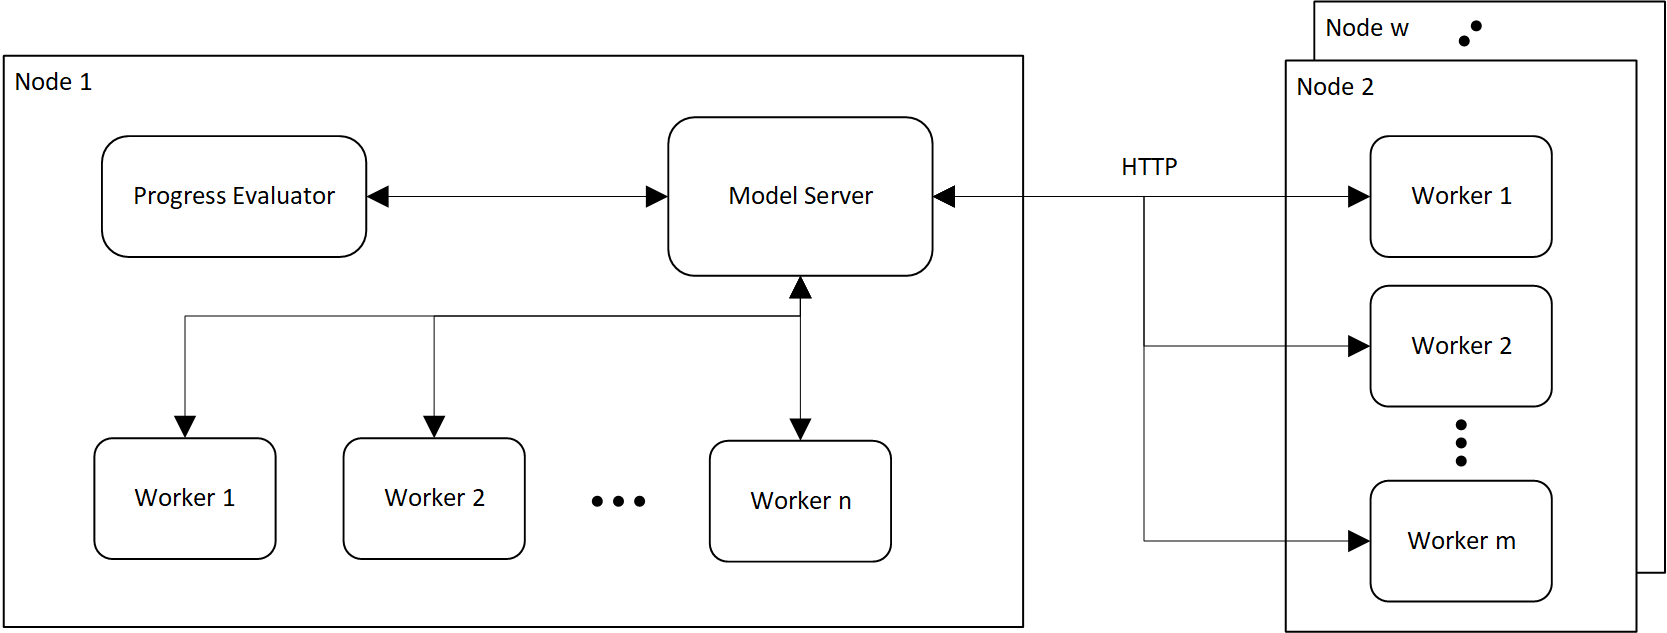
\includegraphics[width=400pt]{images/visio/architecture.png}
	\caption{Illustration of distributed architectures with main node (node 1) and several additional nodes (2-w) connected over HTTP.}
	\label{dist_architecture_img}
\end{figure}


The Flatland environment is running on each cpu core and the results are sent to a web server which updates the model and sent the updated neural network weights back to the client. \\
The reason why we are using CPU cores over GPU performance is that the reinforcement algorithm A3C performs better on CPUs instead of GPUs. \\  %TODO: Grund eventuell erweitern?

All experiments (mentioned in \autoref{enhanced_observations}) are made on a Openstack Machine with 8 CPU cores and 64Gb memory.
Each experiment ran for 12 hours.\\

We ran an experiment to compare the learning progress between a single worker and 7 workers.\\
The experiment shows that the learning progress with 7 workers is over 2.5 times faster than the learning progress with a single worker.\\
It also shows that the learning curve fluctuates more with a higher amount of workers.\\
%TODO: Update plot with 55 workers and compare it.
%TODO: Fix problem with misplaced image.

\begin{figure}
	\begin{center}
		%% Creator: Matplotlib, PGF backend
%%
%% To include the figure in your LaTeX document, write
%%   \input{<filename>.pgf}
%%
%% Make sure the required packages are loaded in your preamble
%%   \usepackage{pgf}
%%
%% Figures using additional raster images can only be included by \input if
%% they are in the same directory as the main LaTeX file. For loading figures
%% from other directories you can use the `import` package
%%   \usepackage{import}
%% and then include the figures with
%%   \import{<path to file>}{<filename>.pgf}
%%
%% Matplotlib used the following preamble
%%   \usepackage{fontspec}
%%
\begingroup%
\makeatletter%
\begin{pgfpicture}%
\pgfpathrectangle{\pgfpointorigin}{\pgfqpoint{5.000000in}{3.000000in}}%
\pgfusepath{use as bounding box, clip}%
\begin{pgfscope}%
\pgfsetbuttcap%
\pgfsetmiterjoin%
\definecolor{currentfill}{rgb}{1.000000,1.000000,1.000000}%
\pgfsetfillcolor{currentfill}%
\pgfsetlinewidth{0.000000pt}%
\definecolor{currentstroke}{rgb}{1.000000,1.000000,1.000000}%
\pgfsetstrokecolor{currentstroke}%
\pgfsetdash{}{0pt}%
\pgfpathmoveto{\pgfqpoint{0.000000in}{0.000000in}}%
\pgfpathlineto{\pgfqpoint{5.000000in}{0.000000in}}%
\pgfpathlineto{\pgfqpoint{5.000000in}{3.000000in}}%
\pgfpathlineto{\pgfqpoint{0.000000in}{3.000000in}}%
\pgfpathclose%
\pgfusepath{fill}%
\end{pgfscope}%
\begin{pgfscope}%
\pgfsetbuttcap%
\pgfsetmiterjoin%
\definecolor{currentfill}{rgb}{1.000000,1.000000,1.000000}%
\pgfsetfillcolor{currentfill}%
\pgfsetlinewidth{0.000000pt}%
\definecolor{currentstroke}{rgb}{0.000000,0.000000,0.000000}%
\pgfsetstrokecolor{currentstroke}%
\pgfsetstrokeopacity{0.000000}%
\pgfsetdash{}{0pt}%
\pgfpathmoveto{\pgfqpoint{0.568195in}{0.732921in}}%
\pgfpathlineto{\pgfqpoint{4.850000in}{0.732921in}}%
\pgfpathlineto{\pgfqpoint{4.850000in}{2.850000in}}%
\pgfpathlineto{\pgfqpoint{0.568195in}{2.850000in}}%
\pgfpathclose%
\pgfusepath{fill}%
\end{pgfscope}%
\begin{pgfscope}%
\pgfsetbuttcap%
\pgfsetroundjoin%
\definecolor{currentfill}{rgb}{0.000000,0.000000,0.000000}%
\pgfsetfillcolor{currentfill}%
\pgfsetlinewidth{0.803000pt}%
\definecolor{currentstroke}{rgb}{0.000000,0.000000,0.000000}%
\pgfsetstrokecolor{currentstroke}%
\pgfsetdash{}{0pt}%
\pgfsys@defobject{currentmarker}{\pgfqpoint{0.000000in}{-0.048611in}}{\pgfqpoint{0.000000in}{0.000000in}}{%
\pgfpathmoveto{\pgfqpoint{0.000000in}{0.000000in}}%
\pgfpathlineto{\pgfqpoint{0.000000in}{-0.048611in}}%
\pgfusepath{stroke,fill}%
}%
\begin{pgfscope}%
\pgfsys@transformshift{0.762822in}{0.732921in}%
\pgfsys@useobject{currentmarker}{}%
\end{pgfscope}%
\end{pgfscope}%
\begin{pgfscope}%
\definecolor{textcolor}{rgb}{0.000000,0.000000,0.000000}%
\pgfsetstrokecolor{textcolor}%
\pgfsetfillcolor{textcolor}%
\pgftext[x=0.408473in,y=0.355418in,left,base,rotate=30.000000]{\color{textcolor}\rmfamily\fontsize{10.000000}{12.000000}\selectfont 00:00h}%
\end{pgfscope}%
\begin{pgfscope}%
\pgfsetbuttcap%
\pgfsetroundjoin%
\definecolor{currentfill}{rgb}{0.000000,0.000000,0.000000}%
\pgfsetfillcolor{currentfill}%
\pgfsetlinewidth{0.803000pt}%
\definecolor{currentstroke}{rgb}{0.000000,0.000000,0.000000}%
\pgfsetstrokecolor{currentstroke}%
\pgfsetdash{}{0pt}%
\pgfsys@defobject{currentmarker}{\pgfqpoint{0.000000in}{-0.048611in}}{\pgfqpoint{0.000000in}{0.000000in}}{%
\pgfpathmoveto{\pgfqpoint{0.000000in}{0.000000in}}%
\pgfpathlineto{\pgfqpoint{0.000000in}{-0.048611in}}%
\pgfusepath{stroke,fill}%
}%
\begin{pgfscope}%
\pgfsys@transformshift{1.414405in}{0.732921in}%
\pgfsys@useobject{currentmarker}{}%
\end{pgfscope}%
\end{pgfscope}%
\begin{pgfscope}%
\definecolor{textcolor}{rgb}{0.000000,0.000000,0.000000}%
\pgfsetstrokecolor{textcolor}%
\pgfsetfillcolor{textcolor}%
\pgftext[x=1.060056in,y=0.355418in,left,base,rotate=30.000000]{\color{textcolor}\rmfamily\fontsize{10.000000}{12.000000}\selectfont 02:00h}%
\end{pgfscope}%
\begin{pgfscope}%
\pgfsetbuttcap%
\pgfsetroundjoin%
\definecolor{currentfill}{rgb}{0.000000,0.000000,0.000000}%
\pgfsetfillcolor{currentfill}%
\pgfsetlinewidth{0.803000pt}%
\definecolor{currentstroke}{rgb}{0.000000,0.000000,0.000000}%
\pgfsetstrokecolor{currentstroke}%
\pgfsetdash{}{0pt}%
\pgfsys@defobject{currentmarker}{\pgfqpoint{0.000000in}{-0.048611in}}{\pgfqpoint{0.000000in}{0.000000in}}{%
\pgfpathmoveto{\pgfqpoint{0.000000in}{0.000000in}}%
\pgfpathlineto{\pgfqpoint{0.000000in}{-0.048611in}}%
\pgfusepath{stroke,fill}%
}%
\begin{pgfscope}%
\pgfsys@transformshift{2.065988in}{0.732921in}%
\pgfsys@useobject{currentmarker}{}%
\end{pgfscope}%
\end{pgfscope}%
\begin{pgfscope}%
\definecolor{textcolor}{rgb}{0.000000,0.000000,0.000000}%
\pgfsetstrokecolor{textcolor}%
\pgfsetfillcolor{textcolor}%
\pgftext[x=1.711639in,y=0.355418in,left,base,rotate=30.000000]{\color{textcolor}\rmfamily\fontsize{10.000000}{12.000000}\selectfont 04:00h}%
\end{pgfscope}%
\begin{pgfscope}%
\pgfsetbuttcap%
\pgfsetroundjoin%
\definecolor{currentfill}{rgb}{0.000000,0.000000,0.000000}%
\pgfsetfillcolor{currentfill}%
\pgfsetlinewidth{0.803000pt}%
\definecolor{currentstroke}{rgb}{0.000000,0.000000,0.000000}%
\pgfsetstrokecolor{currentstroke}%
\pgfsetdash{}{0pt}%
\pgfsys@defobject{currentmarker}{\pgfqpoint{0.000000in}{-0.048611in}}{\pgfqpoint{0.000000in}{0.000000in}}{%
\pgfpathmoveto{\pgfqpoint{0.000000in}{0.000000in}}%
\pgfpathlineto{\pgfqpoint{0.000000in}{-0.048611in}}%
\pgfusepath{stroke,fill}%
}%
\begin{pgfscope}%
\pgfsys@transformshift{2.717571in}{0.732921in}%
\pgfsys@useobject{currentmarker}{}%
\end{pgfscope}%
\end{pgfscope}%
\begin{pgfscope}%
\definecolor{textcolor}{rgb}{0.000000,0.000000,0.000000}%
\pgfsetstrokecolor{textcolor}%
\pgfsetfillcolor{textcolor}%
\pgftext[x=2.363222in,y=0.355418in,left,base,rotate=30.000000]{\color{textcolor}\rmfamily\fontsize{10.000000}{12.000000}\selectfont 06:00h}%
\end{pgfscope}%
\begin{pgfscope}%
\pgfsetbuttcap%
\pgfsetroundjoin%
\definecolor{currentfill}{rgb}{0.000000,0.000000,0.000000}%
\pgfsetfillcolor{currentfill}%
\pgfsetlinewidth{0.803000pt}%
\definecolor{currentstroke}{rgb}{0.000000,0.000000,0.000000}%
\pgfsetstrokecolor{currentstroke}%
\pgfsetdash{}{0pt}%
\pgfsys@defobject{currentmarker}{\pgfqpoint{0.000000in}{-0.048611in}}{\pgfqpoint{0.000000in}{0.000000in}}{%
\pgfpathmoveto{\pgfqpoint{0.000000in}{0.000000in}}%
\pgfpathlineto{\pgfqpoint{0.000000in}{-0.048611in}}%
\pgfusepath{stroke,fill}%
}%
\begin{pgfscope}%
\pgfsys@transformshift{3.369154in}{0.732921in}%
\pgfsys@useobject{currentmarker}{}%
\end{pgfscope}%
\end{pgfscope}%
\begin{pgfscope}%
\definecolor{textcolor}{rgb}{0.000000,0.000000,0.000000}%
\pgfsetstrokecolor{textcolor}%
\pgfsetfillcolor{textcolor}%
\pgftext[x=3.014805in,y=0.355418in,left,base,rotate=30.000000]{\color{textcolor}\rmfamily\fontsize{10.000000}{12.000000}\selectfont 08:00h}%
\end{pgfscope}%
\begin{pgfscope}%
\pgfsetbuttcap%
\pgfsetroundjoin%
\definecolor{currentfill}{rgb}{0.000000,0.000000,0.000000}%
\pgfsetfillcolor{currentfill}%
\pgfsetlinewidth{0.803000pt}%
\definecolor{currentstroke}{rgb}{0.000000,0.000000,0.000000}%
\pgfsetstrokecolor{currentstroke}%
\pgfsetdash{}{0pt}%
\pgfsys@defobject{currentmarker}{\pgfqpoint{0.000000in}{-0.048611in}}{\pgfqpoint{0.000000in}{0.000000in}}{%
\pgfpathmoveto{\pgfqpoint{0.000000in}{0.000000in}}%
\pgfpathlineto{\pgfqpoint{0.000000in}{-0.048611in}}%
\pgfusepath{stroke,fill}%
}%
\begin{pgfscope}%
\pgfsys@transformshift{4.020737in}{0.732921in}%
\pgfsys@useobject{currentmarker}{}%
\end{pgfscope}%
\end{pgfscope}%
\begin{pgfscope}%
\definecolor{textcolor}{rgb}{0.000000,0.000000,0.000000}%
\pgfsetstrokecolor{textcolor}%
\pgfsetfillcolor{textcolor}%
\pgftext[x=3.666388in,y=0.355418in,left,base,rotate=30.000000]{\color{textcolor}\rmfamily\fontsize{10.000000}{12.000000}\selectfont 10:00h}%
\end{pgfscope}%
\begin{pgfscope}%
\pgfsetbuttcap%
\pgfsetroundjoin%
\definecolor{currentfill}{rgb}{0.000000,0.000000,0.000000}%
\pgfsetfillcolor{currentfill}%
\pgfsetlinewidth{0.803000pt}%
\definecolor{currentstroke}{rgb}{0.000000,0.000000,0.000000}%
\pgfsetstrokecolor{currentstroke}%
\pgfsetdash{}{0pt}%
\pgfsys@defobject{currentmarker}{\pgfqpoint{0.000000in}{-0.048611in}}{\pgfqpoint{0.000000in}{0.000000in}}{%
\pgfpathmoveto{\pgfqpoint{0.000000in}{0.000000in}}%
\pgfpathlineto{\pgfqpoint{0.000000in}{-0.048611in}}%
\pgfusepath{stroke,fill}%
}%
\begin{pgfscope}%
\pgfsys@transformshift{4.672320in}{0.732921in}%
\pgfsys@useobject{currentmarker}{}%
\end{pgfscope}%
\end{pgfscope}%
\begin{pgfscope}%
\definecolor{textcolor}{rgb}{0.000000,0.000000,0.000000}%
\pgfsetstrokecolor{textcolor}%
\pgfsetfillcolor{textcolor}%
\pgftext[x=4.317971in,y=0.355418in,left,base,rotate=30.000000]{\color{textcolor}\rmfamily\fontsize{10.000000}{12.000000}\selectfont 12:00h}%
\end{pgfscope}%
\begin{pgfscope}%
\definecolor{textcolor}{rgb}{0.000000,0.000000,0.000000}%
\pgfsetstrokecolor{textcolor}%
\pgfsetfillcolor{textcolor}%
\pgftext[x=2.709097in,y=0.276528in,,top]{\color{textcolor}\rmfamily\fontsize{10.000000}{12.000000}\selectfont Hours of training}%
\end{pgfscope}%
\begin{pgfscope}%
\pgfsetbuttcap%
\pgfsetroundjoin%
\definecolor{currentfill}{rgb}{0.000000,0.000000,0.000000}%
\pgfsetfillcolor{currentfill}%
\pgfsetlinewidth{0.803000pt}%
\definecolor{currentstroke}{rgb}{0.000000,0.000000,0.000000}%
\pgfsetstrokecolor{currentstroke}%
\pgfsetdash{}{0pt}%
\pgfsys@defobject{currentmarker}{\pgfqpoint{-0.048611in}{0.000000in}}{\pgfqpoint{0.000000in}{0.000000in}}{%
\pgfpathmoveto{\pgfqpoint{0.000000in}{0.000000in}}%
\pgfpathlineto{\pgfqpoint{-0.048611in}{0.000000in}}%
\pgfusepath{stroke,fill}%
}%
\begin{pgfscope}%
\pgfsys@transformshift{0.568195in}{0.751389in}%
\pgfsys@useobject{currentmarker}{}%
\end{pgfscope}%
\end{pgfscope}%
\begin{pgfscope}%
\definecolor{textcolor}{rgb}{0.000000,0.000000,0.000000}%
\pgfsetstrokecolor{textcolor}%
\pgfsetfillcolor{textcolor}%
\pgftext[x=0.401528in,y=0.703195in,left,base]{\color{textcolor}\rmfamily\fontsize{10.000000}{12.000000}\selectfont \(\displaystyle 0\)}%
\end{pgfscope}%
\begin{pgfscope}%
\pgfsetbuttcap%
\pgfsetroundjoin%
\definecolor{currentfill}{rgb}{0.000000,0.000000,0.000000}%
\pgfsetfillcolor{currentfill}%
\pgfsetlinewidth{0.803000pt}%
\definecolor{currentstroke}{rgb}{0.000000,0.000000,0.000000}%
\pgfsetstrokecolor{currentstroke}%
\pgfsetdash{}{0pt}%
\pgfsys@defobject{currentmarker}{\pgfqpoint{-0.048611in}{0.000000in}}{\pgfqpoint{0.000000in}{0.000000in}}{%
\pgfpathmoveto{\pgfqpoint{0.000000in}{0.000000in}}%
\pgfpathlineto{\pgfqpoint{-0.048611in}{0.000000in}}%
\pgfusepath{stroke,fill}%
}%
\begin{pgfscope}%
\pgfsys@transformshift{0.568195in}{1.140201in}%
\pgfsys@useobject{currentmarker}{}%
\end{pgfscope}%
\end{pgfscope}%
\begin{pgfscope}%
\definecolor{textcolor}{rgb}{0.000000,0.000000,0.000000}%
\pgfsetstrokecolor{textcolor}%
\pgfsetfillcolor{textcolor}%
\pgftext[x=0.401528in,y=1.092006in,left,base]{\color{textcolor}\rmfamily\fontsize{10.000000}{12.000000}\selectfont \(\displaystyle 2\)}%
\end{pgfscope}%
\begin{pgfscope}%
\pgfsetbuttcap%
\pgfsetroundjoin%
\definecolor{currentfill}{rgb}{0.000000,0.000000,0.000000}%
\pgfsetfillcolor{currentfill}%
\pgfsetlinewidth{0.803000pt}%
\definecolor{currentstroke}{rgb}{0.000000,0.000000,0.000000}%
\pgfsetstrokecolor{currentstroke}%
\pgfsetdash{}{0pt}%
\pgfsys@defobject{currentmarker}{\pgfqpoint{-0.048611in}{0.000000in}}{\pgfqpoint{0.000000in}{0.000000in}}{%
\pgfpathmoveto{\pgfqpoint{0.000000in}{0.000000in}}%
\pgfpathlineto{\pgfqpoint{-0.048611in}{0.000000in}}%
\pgfusepath{stroke,fill}%
}%
\begin{pgfscope}%
\pgfsys@transformshift{0.568195in}{1.529012in}%
\pgfsys@useobject{currentmarker}{}%
\end{pgfscope}%
\end{pgfscope}%
\begin{pgfscope}%
\definecolor{textcolor}{rgb}{0.000000,0.000000,0.000000}%
\pgfsetstrokecolor{textcolor}%
\pgfsetfillcolor{textcolor}%
\pgftext[x=0.401528in,y=1.480818in,left,base]{\color{textcolor}\rmfamily\fontsize{10.000000}{12.000000}\selectfont \(\displaystyle 4\)}%
\end{pgfscope}%
\begin{pgfscope}%
\pgfsetbuttcap%
\pgfsetroundjoin%
\definecolor{currentfill}{rgb}{0.000000,0.000000,0.000000}%
\pgfsetfillcolor{currentfill}%
\pgfsetlinewidth{0.803000pt}%
\definecolor{currentstroke}{rgb}{0.000000,0.000000,0.000000}%
\pgfsetstrokecolor{currentstroke}%
\pgfsetdash{}{0pt}%
\pgfsys@defobject{currentmarker}{\pgfqpoint{-0.048611in}{0.000000in}}{\pgfqpoint{0.000000in}{0.000000in}}{%
\pgfpathmoveto{\pgfqpoint{0.000000in}{0.000000in}}%
\pgfpathlineto{\pgfqpoint{-0.048611in}{0.000000in}}%
\pgfusepath{stroke,fill}%
}%
\begin{pgfscope}%
\pgfsys@transformshift{0.568195in}{1.917824in}%
\pgfsys@useobject{currentmarker}{}%
\end{pgfscope}%
\end{pgfscope}%
\begin{pgfscope}%
\definecolor{textcolor}{rgb}{0.000000,0.000000,0.000000}%
\pgfsetstrokecolor{textcolor}%
\pgfsetfillcolor{textcolor}%
\pgftext[x=0.401528in,y=1.869630in,left,base]{\color{textcolor}\rmfamily\fontsize{10.000000}{12.000000}\selectfont \(\displaystyle 6\)}%
\end{pgfscope}%
\begin{pgfscope}%
\pgfsetbuttcap%
\pgfsetroundjoin%
\definecolor{currentfill}{rgb}{0.000000,0.000000,0.000000}%
\pgfsetfillcolor{currentfill}%
\pgfsetlinewidth{0.803000pt}%
\definecolor{currentstroke}{rgb}{0.000000,0.000000,0.000000}%
\pgfsetstrokecolor{currentstroke}%
\pgfsetdash{}{0pt}%
\pgfsys@defobject{currentmarker}{\pgfqpoint{-0.048611in}{0.000000in}}{\pgfqpoint{0.000000in}{0.000000in}}{%
\pgfpathmoveto{\pgfqpoint{0.000000in}{0.000000in}}%
\pgfpathlineto{\pgfqpoint{-0.048611in}{0.000000in}}%
\pgfusepath{stroke,fill}%
}%
\begin{pgfscope}%
\pgfsys@transformshift{0.568195in}{2.306636in}%
\pgfsys@useobject{currentmarker}{}%
\end{pgfscope}%
\end{pgfscope}%
\begin{pgfscope}%
\definecolor{textcolor}{rgb}{0.000000,0.000000,0.000000}%
\pgfsetstrokecolor{textcolor}%
\pgfsetfillcolor{textcolor}%
\pgftext[x=0.401528in,y=2.258441in,left,base]{\color{textcolor}\rmfamily\fontsize{10.000000}{12.000000}\selectfont \(\displaystyle 8\)}%
\end{pgfscope}%
\begin{pgfscope}%
\pgfsetbuttcap%
\pgfsetroundjoin%
\definecolor{currentfill}{rgb}{0.000000,0.000000,0.000000}%
\pgfsetfillcolor{currentfill}%
\pgfsetlinewidth{0.803000pt}%
\definecolor{currentstroke}{rgb}{0.000000,0.000000,0.000000}%
\pgfsetstrokecolor{currentstroke}%
\pgfsetdash{}{0pt}%
\pgfsys@defobject{currentmarker}{\pgfqpoint{-0.048611in}{0.000000in}}{\pgfqpoint{0.000000in}{0.000000in}}{%
\pgfpathmoveto{\pgfqpoint{0.000000in}{0.000000in}}%
\pgfpathlineto{\pgfqpoint{-0.048611in}{0.000000in}}%
\pgfusepath{stroke,fill}%
}%
\begin{pgfscope}%
\pgfsys@transformshift{0.568195in}{2.695447in}%
\pgfsys@useobject{currentmarker}{}%
\end{pgfscope}%
\end{pgfscope}%
\begin{pgfscope}%
\definecolor{textcolor}{rgb}{0.000000,0.000000,0.000000}%
\pgfsetstrokecolor{textcolor}%
\pgfsetfillcolor{textcolor}%
\pgftext[x=0.332083in,y=2.647253in,left,base]{\color{textcolor}\rmfamily\fontsize{10.000000}{12.000000}\selectfont \(\displaystyle 10\)}%
\end{pgfscope}%
\begin{pgfscope}%
\definecolor{textcolor}{rgb}{0.000000,0.000000,0.000000}%
\pgfsetstrokecolor{textcolor}%
\pgfsetfillcolor{textcolor}%
\pgftext[x=0.276528in,y=1.791460in,,bottom,rotate=90.000000]{\color{textcolor}\rmfamily\fontsize{10.000000}{12.000000}\selectfont Number of agents arriving}%
\end{pgfscope}%
\begin{pgfscope}%
\pgfpathrectangle{\pgfqpoint{0.568195in}{0.732921in}}{\pgfqpoint{4.281805in}{2.117079in}}%
\pgfusepath{clip}%
\pgfsetrectcap%
\pgfsetroundjoin%
\pgfsetlinewidth{1.505625pt}%
\definecolor{currentstroke}{rgb}{0.121569,0.466667,0.705882}%
\pgfsetstrokecolor{currentstroke}%
\pgfsetdash{}{0pt}%
\pgfpathmoveto{\pgfqpoint{0.762822in}{0.897193in}}%
\pgfpathlineto{\pgfqpoint{0.798913in}{0.829151in}}%
\pgfpathlineto{\pgfqpoint{0.838464in}{0.858312in}}%
\pgfpathlineto{\pgfqpoint{0.877563in}{0.945795in}}%
\pgfpathlineto{\pgfqpoint{0.916621in}{1.013837in}}%
\pgfpathlineto{\pgfqpoint{0.953962in}{1.266565in}}%
\pgfpathlineto{\pgfqpoint{0.990097in}{1.373488in}}%
\pgfpathlineto{\pgfqpoint{1.024590in}{1.781740in}}%
\pgfpathlineto{\pgfqpoint{1.055118in}{1.995586in}}%
\pgfpathlineto{\pgfqpoint{1.085139in}{1.723418in}}%
\pgfpathlineto{\pgfqpoint{1.117316in}{1.966426in}}%
\pgfpathlineto{\pgfqpoint{1.146193in}{2.092789in}}%
\pgfpathlineto{\pgfqpoint{1.175301in}{2.394118in}}%
\pgfpathlineto{\pgfqpoint{1.203923in}{2.228873in}}%
\pgfpathlineto{\pgfqpoint{1.232459in}{2.277475in}}%
\pgfpathlineto{\pgfqpoint{1.260998in}{2.335797in}}%
\pgfpathlineto{\pgfqpoint{1.289573in}{1.849782in}}%
\pgfpathlineto{\pgfqpoint{1.320072in}{2.287195in}}%
\pgfpathlineto{\pgfqpoint{1.346641in}{1.820621in}}%
\pgfpathlineto{\pgfqpoint{1.378822in}{2.384398in}}%
\pgfpathlineto{\pgfqpoint{1.406464in}{2.131670in}}%
\pgfpathlineto{\pgfqpoint{1.435222in}{2.151111in}}%
\pgfpathlineto{\pgfqpoint{1.464793in}{2.520482in}}%
\pgfpathlineto{\pgfqpoint{1.491531in}{2.326076in}}%
\pgfpathlineto{\pgfqpoint{1.519563in}{2.510762in}}%
\pgfpathlineto{\pgfqpoint{1.548531in}{2.228873in}}%
\pgfpathlineto{\pgfqpoint{1.578073in}{2.355237in}}%
\pgfpathlineto{\pgfqpoint{1.606990in}{2.413559in}}%
\pgfpathlineto{\pgfqpoint{1.633884in}{2.442720in}}%
\pgfpathlineto{\pgfqpoint{1.661437in}{2.296915in}}%
\pgfpathlineto{\pgfqpoint{1.690225in}{2.432999in}}%
\pgfpathlineto{\pgfqpoint{1.718908in}{2.374678in}}%
\pgfpathlineto{\pgfqpoint{1.746907in}{2.355237in}}%
\pgfpathlineto{\pgfqpoint{1.773753in}{2.355237in}}%
\pgfpathlineto{\pgfqpoint{1.801930in}{2.345517in}}%
\pgfpathlineto{\pgfqpoint{1.829170in}{2.462160in}}%
\pgfpathlineto{\pgfqpoint{1.855447in}{2.491321in}}%
\pgfpathlineto{\pgfqpoint{1.882461in}{2.335797in}}%
\pgfpathlineto{\pgfqpoint{1.909222in}{2.345517in}}%
\pgfpathlineto{\pgfqpoint{1.936530in}{2.598244in}}%
\pgfpathlineto{\pgfqpoint{1.963879in}{2.442720in}}%
\pgfpathlineto{\pgfqpoint{1.991983in}{2.345517in}}%
\pgfpathlineto{\pgfqpoint{2.020650in}{2.199712in}}%
\pgfpathlineto{\pgfqpoint{2.048384in}{2.326076in}}%
\pgfpathlineto{\pgfqpoint{2.078919in}{2.384398in}}%
\pgfpathlineto{\pgfqpoint{2.105310in}{2.539923in}}%
\pgfpathlineto{\pgfqpoint{2.130308in}{2.238594in}}%
\pgfpathlineto{\pgfqpoint{2.157804in}{2.345517in}}%
\pgfpathlineto{\pgfqpoint{2.185398in}{2.364957in}}%
\pgfpathlineto{\pgfqpoint{2.215039in}{2.277475in}}%
\pgfpathlineto{\pgfqpoint{2.243103in}{2.530202in}}%
\pgfpathlineto{\pgfqpoint{2.269788in}{2.306636in}}%
\pgfpathlineto{\pgfqpoint{2.300367in}{2.364957in}}%
\pgfpathlineto{\pgfqpoint{2.328918in}{2.335797in}}%
\pgfpathlineto{\pgfqpoint{2.356453in}{2.569084in}}%
\pgfpathlineto{\pgfqpoint{2.382936in}{2.530202in}}%
\pgfpathlineto{\pgfqpoint{2.409729in}{2.510762in}}%
\pgfpathlineto{\pgfqpoint{2.437782in}{2.403839in}}%
\pgfpathlineto{\pgfqpoint{2.465394in}{2.432999in}}%
\pgfpathlineto{\pgfqpoint{2.492260in}{2.296915in}}%
\pgfpathlineto{\pgfqpoint{2.520493in}{2.423279in}}%
\pgfpathlineto{\pgfqpoint{2.548179in}{2.219153in}}%
\pgfpathlineto{\pgfqpoint{2.576167in}{2.481601in}}%
\pgfpathlineto{\pgfqpoint{2.602342in}{2.306636in}}%
\pgfpathlineto{\pgfqpoint{2.629736in}{2.394118in}}%
\pgfpathlineto{\pgfqpoint{2.657417in}{2.627405in}}%
\pgfpathlineto{\pgfqpoint{2.683507in}{2.452440in}}%
\pgfpathlineto{\pgfqpoint{2.712108in}{2.510762in}}%
\pgfpathlineto{\pgfqpoint{2.738990in}{2.432999in}}%
\pgfpathlineto{\pgfqpoint{2.766410in}{2.471881in}}%
\pgfpathlineto{\pgfqpoint{2.793995in}{2.326076in}}%
\pgfpathlineto{\pgfqpoint{2.821966in}{2.394118in}}%
\pgfpathlineto{\pgfqpoint{2.850133in}{2.491321in}}%
\pgfpathlineto{\pgfqpoint{2.876676in}{2.063628in}}%
\pgfpathlineto{\pgfqpoint{2.907107in}{2.326076in}}%
\pgfpathlineto{\pgfqpoint{2.935516in}{2.277475in}}%
\pgfpathlineto{\pgfqpoint{2.962918in}{2.316356in}}%
\pgfpathlineto{\pgfqpoint{2.991666in}{2.520482in}}%
\pgfpathlineto{\pgfqpoint{3.019673in}{2.180272in}}%
\pgfpathlineto{\pgfqpoint{3.047513in}{2.569084in}}%
\pgfpathlineto{\pgfqpoint{3.073414in}{2.510762in}}%
\pgfpathlineto{\pgfqpoint{3.099360in}{2.374678in}}%
\pgfpathlineto{\pgfqpoint{3.153310in}{2.452440in}}%
\pgfpathlineto{\pgfqpoint{3.181220in}{2.403839in}}%
\pgfpathlineto{\pgfqpoint{3.208198in}{2.277475in}}%
\pgfpathlineto{\pgfqpoint{3.235853in}{2.432999in}}%
\pgfpathlineto{\pgfqpoint{3.264333in}{2.471881in}}%
\pgfpathlineto{\pgfqpoint{3.290655in}{2.345517in}}%
\pgfpathlineto{\pgfqpoint{3.318177in}{2.316356in}}%
\pgfpathlineto{\pgfqpoint{3.346659in}{2.588524in}}%
\pgfpathlineto{\pgfqpoint{3.373306in}{2.481601in}}%
\pgfpathlineto{\pgfqpoint{3.400072in}{2.335797in}}%
\pgfpathlineto{\pgfqpoint{3.427822in}{2.394118in}}%
\pgfpathlineto{\pgfqpoint{3.454975in}{2.403839in}}%
\pgfpathlineto{\pgfqpoint{3.481972in}{2.559363in}}%
\pgfpathlineto{\pgfqpoint{3.509542in}{2.530202in}}%
\pgfpathlineto{\pgfqpoint{3.537253in}{2.520482in}}%
\pgfpathlineto{\pgfqpoint{3.563799in}{2.277475in}}%
\pgfpathlineto{\pgfqpoint{3.592722in}{2.432999in}}%
\pgfpathlineto{\pgfqpoint{3.618971in}{2.549643in}}%
\pgfpathlineto{\pgfqpoint{3.645122in}{2.287195in}}%
\pgfpathlineto{\pgfqpoint{3.673400in}{2.248314in}}%
\pgfpathlineto{\pgfqpoint{3.701096in}{2.510762in}}%
\pgfpathlineto{\pgfqpoint{3.728120in}{2.364957in}}%
\pgfpathlineto{\pgfqpoint{3.755687in}{2.452440in}}%
\pgfpathlineto{\pgfqpoint{3.782750in}{2.238594in}}%
\pgfpathlineto{\pgfqpoint{3.811067in}{2.209433in}}%
\pgfpathlineto{\pgfqpoint{3.840710in}{2.578804in}}%
\pgfpathlineto{\pgfqpoint{3.866715in}{2.491321in}}%
\pgfpathlineto{\pgfqpoint{3.893436in}{2.335797in}}%
\pgfpathlineto{\pgfqpoint{3.921302in}{2.471881in}}%
\pgfpathlineto{\pgfqpoint{3.947594in}{2.199712in}}%
\pgfpathlineto{\pgfqpoint{3.975254in}{2.471881in}}%
\pgfpathlineto{\pgfqpoint{4.003233in}{2.559363in}}%
\pgfpathlineto{\pgfqpoint{4.029050in}{2.569084in}}%
\pgfpathlineto{\pgfqpoint{4.054642in}{2.607965in}}%
\pgfpathlineto{\pgfqpoint{4.082523in}{2.510762in}}%
\pgfpathlineto{\pgfqpoint{4.110493in}{2.384398in}}%
\pgfpathlineto{\pgfqpoint{4.136649in}{2.296915in}}%
\pgfpathlineto{\pgfqpoint{4.163848in}{2.627405in}}%
\pgfpathlineto{\pgfqpoint{4.189782in}{2.258034in}}%
\pgfpathlineto{\pgfqpoint{4.218702in}{2.267755in}}%
\pgfpathlineto{\pgfqpoint{4.248091in}{2.141391in}}%
\pgfpathlineto{\pgfqpoint{4.276166in}{2.326076in}}%
\pgfpathlineto{\pgfqpoint{4.304088in}{2.481601in}}%
\pgfpathlineto{\pgfqpoint{4.329619in}{2.432999in}}%
\pgfpathlineto{\pgfqpoint{4.357939in}{2.520482in}}%
\pgfpathlineto{\pgfqpoint{4.384016in}{2.637126in}}%
\pgfpathlineto{\pgfqpoint{4.409011in}{2.666286in}}%
\pgfpathlineto{\pgfqpoint{4.436215in}{2.471881in}}%
\pgfpathlineto{\pgfqpoint{4.462184in}{2.471881in}}%
\pgfpathlineto{\pgfqpoint{4.489481in}{2.491321in}}%
\pgfpathlineto{\pgfqpoint{4.515945in}{2.753769in}}%
\pgfpathlineto{\pgfqpoint{4.541490in}{2.423279in}}%
\pgfpathlineto{\pgfqpoint{4.568754in}{2.442720in}}%
\pgfpathlineto{\pgfqpoint{4.596372in}{2.501042in}}%
\pgfpathlineto{\pgfqpoint{4.623473in}{2.637126in}}%
\pgfpathlineto{\pgfqpoint{4.649379in}{2.561793in}}%
\pgfpathlineto{\pgfqpoint{4.649379in}{2.561793in}}%
\pgfusepath{stroke}%
\end{pgfscope}%
\begin{pgfscope}%
\pgfpathrectangle{\pgfqpoint{0.568195in}{0.732921in}}{\pgfqpoint{4.281805in}{2.117079in}}%
\pgfusepath{clip}%
\pgfsetrectcap%
\pgfsetroundjoin%
\pgfsetlinewidth{1.505625pt}%
\definecolor{currentstroke}{rgb}{1.000000,0.498039,0.054902}%
\pgfsetstrokecolor{currentstroke}%
\pgfsetdash{}{0pt}%
\pgfpathmoveto{\pgfqpoint{0.762822in}{0.829151in}}%
\pgfpathlineto{\pgfqpoint{0.803374in}{0.848592in}}%
\pgfpathlineto{\pgfqpoint{0.842171in}{0.897193in}}%
\pgfpathlineto{\pgfqpoint{0.879830in}{0.877753in}}%
\pgfpathlineto{\pgfqpoint{0.916417in}{0.838872in}}%
\pgfpathlineto{\pgfqpoint{0.954689in}{0.926354in}}%
\pgfpathlineto{\pgfqpoint{0.990752in}{0.916634in}}%
\pgfpathlineto{\pgfqpoint{1.029518in}{0.897193in}}%
\pgfpathlineto{\pgfqpoint{1.066494in}{0.858312in}}%
\pgfpathlineto{\pgfqpoint{1.102562in}{0.926354in}}%
\pgfpathlineto{\pgfqpoint{1.139654in}{0.897193in}}%
\pgfpathlineto{\pgfqpoint{1.173908in}{0.877753in}}%
\pgfpathlineto{\pgfqpoint{1.210496in}{0.965235in}}%
\pgfpathlineto{\pgfqpoint{1.246268in}{0.877753in}}%
\pgfpathlineto{\pgfqpoint{1.282529in}{0.897193in}}%
\pgfpathlineto{\pgfqpoint{1.318462in}{0.936075in}}%
\pgfpathlineto{\pgfqpoint{1.355112in}{0.994396in}}%
\pgfpathlineto{\pgfqpoint{1.391573in}{0.994396in}}%
\pgfpathlineto{\pgfqpoint{1.428185in}{0.906914in}}%
\pgfpathlineto{\pgfqpoint{1.464156in}{1.033278in}}%
\pgfpathlineto{\pgfqpoint{1.500457in}{1.013837in}}%
\pgfpathlineto{\pgfqpoint{1.534730in}{1.130480in}}%
\pgfpathlineto{\pgfqpoint{1.573088in}{1.111040in}}%
\pgfpathlineto{\pgfqpoint{1.611757in}{1.256844in}}%
\pgfpathlineto{\pgfqpoint{1.649025in}{1.305446in}}%
\pgfpathlineto{\pgfqpoint{1.683083in}{1.208243in}}%
\pgfpathlineto{\pgfqpoint{1.720002in}{1.286005in}}%
\pgfpathlineto{\pgfqpoint{1.756975in}{1.373488in}}%
\pgfpathlineto{\pgfqpoint{1.791431in}{1.548453in}}%
\pgfpathlineto{\pgfqpoint{1.823243in}{1.451250in}}%
\pgfpathlineto{\pgfqpoint{1.858532in}{1.373488in}}%
\pgfpathlineto{\pgfqpoint{1.893726in}{1.529012in}}%
\pgfpathlineto{\pgfqpoint{1.929090in}{1.509572in}}%
\pgfpathlineto{\pgfqpoint{1.963527in}{1.558173in}}%
\pgfpathlineto{\pgfqpoint{1.997610in}{1.431809in}}%
\pgfpathlineto{\pgfqpoint{2.032501in}{1.587334in}}%
\pgfpathlineto{\pgfqpoint{2.068896in}{1.597054in}}%
\pgfpathlineto{\pgfqpoint{2.103009in}{1.597054in}}%
\pgfpathlineto{\pgfqpoint{2.136292in}{1.762299in}}%
\pgfpathlineto{\pgfqpoint{2.168303in}{1.772020in}}%
\pgfpathlineto{\pgfqpoint{2.200502in}{1.849782in}}%
\pgfpathlineto{\pgfqpoint{2.233546in}{1.480411in}}%
\pgfpathlineto{\pgfqpoint{2.267925in}{1.723418in}}%
\pgfpathlineto{\pgfqpoint{2.299739in}{1.878943in}}%
\pgfpathlineto{\pgfqpoint{2.332819in}{2.121950in}}%
\pgfpathlineto{\pgfqpoint{2.363323in}{1.908104in}}%
\pgfpathlineto{\pgfqpoint{2.397131in}{1.869223in}}%
\pgfpathlineto{\pgfqpoint{2.431400in}{1.985866in}}%
\pgfpathlineto{\pgfqpoint{2.462464in}{1.995586in}}%
\pgfpathlineto{\pgfqpoint{2.495707in}{2.121950in}}%
\pgfpathlineto{\pgfqpoint{2.525764in}{1.985866in}}%
\pgfpathlineto{\pgfqpoint{2.558193in}{2.015027in}}%
\pgfpathlineto{\pgfqpoint{2.591544in}{1.937265in}}%
\pgfpathlineto{\pgfqpoint{2.622551in}{1.859502in}}%
\pgfpathlineto{\pgfqpoint{2.656293in}{2.005307in}}%
\pgfpathlineto{\pgfqpoint{2.687586in}{1.791460in}}%
\pgfpathlineto{\pgfqpoint{2.720430in}{1.908104in}}%
\pgfpathlineto{\pgfqpoint{2.752189in}{1.869223in}}%
\pgfpathlineto{\pgfqpoint{2.783952in}{1.995586in}}%
\pgfpathlineto{\pgfqpoint{2.815430in}{2.170552in}}%
\pgfpathlineto{\pgfqpoint{2.843882in}{1.849782in}}%
\pgfpathlineto{\pgfqpoint{2.875446in}{1.742859in}}%
\pgfpathlineto{\pgfqpoint{2.908721in}{1.898383in}}%
\pgfpathlineto{\pgfqpoint{2.940626in}{2.189992in}}%
\pgfpathlineto{\pgfqpoint{2.971264in}{2.063628in}}%
\pgfpathlineto{\pgfqpoint{3.001239in}{2.034468in}}%
\pgfpathlineto{\pgfqpoint{3.033515in}{2.238594in}}%
\pgfpathlineto{\pgfqpoint{3.062331in}{1.694257in}}%
\pgfpathlineto{\pgfqpoint{3.095574in}{2.102510in}}%
\pgfpathlineto{\pgfqpoint{3.123598in}{2.141391in}}%
\pgfpathlineto{\pgfqpoint{3.153108in}{1.937265in}}%
\pgfpathlineto{\pgfqpoint{3.183330in}{1.655376in}}%
\pgfpathlineto{\pgfqpoint{3.215132in}{2.141391in}}%
\pgfpathlineto{\pgfqpoint{3.244613in}{2.287195in}}%
\pgfpathlineto{\pgfqpoint{3.273190in}{2.267755in}}%
\pgfpathlineto{\pgfqpoint{3.303588in}{2.238594in}}%
\pgfpathlineto{\pgfqpoint{3.331909in}{2.248314in}}%
\pgfpathlineto{\pgfqpoint{3.360735in}{2.151111in}}%
\pgfpathlineto{\pgfqpoint{3.391367in}{2.073349in}}%
\pgfpathlineto{\pgfqpoint{3.421537in}{2.073349in}}%
\pgfpathlineto{\pgfqpoint{3.453044in}{1.946985in}}%
\pgfpathlineto{\pgfqpoint{3.481919in}{2.306636in}}%
\pgfpathlineto{\pgfqpoint{3.508889in}{2.063628in}}%
\pgfpathlineto{\pgfqpoint{3.539591in}{2.384398in}}%
\pgfpathlineto{\pgfqpoint{3.566736in}{2.151111in}}%
\pgfpathlineto{\pgfqpoint{3.596075in}{2.199712in}}%
\pgfpathlineto{\pgfqpoint{3.625215in}{2.403839in}}%
\pgfpathlineto{\pgfqpoint{3.653755in}{2.083069in}}%
\pgfpathlineto{\pgfqpoint{3.684402in}{2.287195in}}%
\pgfpathlineto{\pgfqpoint{3.712921in}{2.530202in}}%
\pgfpathlineto{\pgfqpoint{3.738425in}{2.510762in}}%
\pgfpathlineto{\pgfqpoint{3.764090in}{2.374678in}}%
\pgfpathlineto{\pgfqpoint{3.790679in}{2.335797in}}%
\pgfpathlineto{\pgfqpoint{3.819410in}{2.345517in}}%
\pgfpathlineto{\pgfqpoint{3.848920in}{2.355237in}}%
\pgfpathlineto{\pgfqpoint{3.878009in}{2.394118in}}%
\pgfpathlineto{\pgfqpoint{3.905496in}{2.462160in}}%
\pgfpathlineto{\pgfqpoint{3.932259in}{2.491321in}}%
\pgfpathlineto{\pgfqpoint{3.958870in}{2.248314in}}%
\pgfpathlineto{\pgfqpoint{3.988039in}{2.462160in}}%
\pgfpathlineto{\pgfqpoint{4.014178in}{2.170552in}}%
\pgfpathlineto{\pgfqpoint{4.044653in}{2.384398in}}%
\pgfpathlineto{\pgfqpoint{4.071407in}{2.316356in}}%
\pgfpathlineto{\pgfqpoint{4.100711in}{2.423279in}}%
\pgfpathlineto{\pgfqpoint{4.127080in}{2.160831in}}%
\pgfpathlineto{\pgfqpoint{4.156855in}{2.569084in}}%
\pgfpathlineto{\pgfqpoint{4.183391in}{2.326076in}}%
\pgfpathlineto{\pgfqpoint{4.211928in}{2.238594in}}%
\pgfpathlineto{\pgfqpoint{4.239348in}{2.403839in}}%
\pgfpathlineto{\pgfqpoint{4.267070in}{2.248314in}}%
\pgfpathlineto{\pgfqpoint{4.295230in}{2.510762in}}%
\pgfpathlineto{\pgfqpoint{4.323267in}{2.355237in}}%
\pgfpathlineto{\pgfqpoint{4.351112in}{2.423279in}}%
\pgfpathlineto{\pgfqpoint{4.378346in}{2.384398in}}%
\pgfpathlineto{\pgfqpoint{4.405460in}{2.462160in}}%
\pgfpathlineto{\pgfqpoint{4.435294in}{2.199712in}}%
\pgfpathlineto{\pgfqpoint{4.463845in}{2.277475in}}%
\pgfpathlineto{\pgfqpoint{4.493999in}{2.423279in}}%
\pgfpathlineto{\pgfqpoint{4.520975in}{2.607965in}}%
\pgfpathlineto{\pgfqpoint{4.546342in}{2.316356in}}%
\pgfpathlineto{\pgfqpoint{4.573017in}{2.316356in}}%
\pgfpathlineto{\pgfqpoint{4.600650in}{2.345517in}}%
\pgfpathlineto{\pgfqpoint{4.629492in}{2.539923in}}%
\pgfpathlineto{\pgfqpoint{4.655372in}{2.575813in}}%
\pgfusepath{stroke}%
\end{pgfscope}%
\begin{pgfscope}%
\pgfsetrectcap%
\pgfsetmiterjoin%
\pgfsetlinewidth{0.803000pt}%
\definecolor{currentstroke}{rgb}{0.000000,0.000000,0.000000}%
\pgfsetstrokecolor{currentstroke}%
\pgfsetdash{}{0pt}%
\pgfpathmoveto{\pgfqpoint{0.568195in}{0.732921in}}%
\pgfpathlineto{\pgfqpoint{0.568195in}{2.850000in}}%
\pgfusepath{stroke}%
\end{pgfscope}%
\begin{pgfscope}%
\pgfsetrectcap%
\pgfsetmiterjoin%
\pgfsetlinewidth{0.803000pt}%
\definecolor{currentstroke}{rgb}{0.000000,0.000000,0.000000}%
\pgfsetstrokecolor{currentstroke}%
\pgfsetdash{}{0pt}%
\pgfpathmoveto{\pgfqpoint{4.850000in}{0.732921in}}%
\pgfpathlineto{\pgfqpoint{4.850000in}{2.850000in}}%
\pgfusepath{stroke}%
\end{pgfscope}%
\begin{pgfscope}%
\pgfsetrectcap%
\pgfsetmiterjoin%
\pgfsetlinewidth{0.803000pt}%
\definecolor{currentstroke}{rgb}{0.000000,0.000000,0.000000}%
\pgfsetstrokecolor{currentstroke}%
\pgfsetdash{}{0pt}%
\pgfpathmoveto{\pgfqpoint{0.568195in}{0.732921in}}%
\pgfpathlineto{\pgfqpoint{4.850000in}{0.732921in}}%
\pgfusepath{stroke}%
\end{pgfscope}%
\begin{pgfscope}%
\pgfsetrectcap%
\pgfsetmiterjoin%
\pgfsetlinewidth{0.803000pt}%
\definecolor{currentstroke}{rgb}{0.000000,0.000000,0.000000}%
\pgfsetstrokecolor{currentstroke}%
\pgfsetdash{}{0pt}%
\pgfpathmoveto{\pgfqpoint{0.568195in}{2.850000in}}%
\pgfpathlineto{\pgfqpoint{4.850000in}{2.850000in}}%
\pgfusepath{stroke}%
\end{pgfscope}%
\begin{pgfscope}%
\pgfsetbuttcap%
\pgfsetmiterjoin%
\definecolor{currentfill}{rgb}{1.000000,1.000000,1.000000}%
\pgfsetfillcolor{currentfill}%
\pgfsetfillopacity{0.800000}%
\pgfsetlinewidth{1.003750pt}%
\definecolor{currentstroke}{rgb}{0.800000,0.800000,0.800000}%
\pgfsetstrokecolor{currentstroke}%
\pgfsetstrokeopacity{0.800000}%
\pgfsetdash{}{0pt}%
\pgfpathmoveto{\pgfqpoint{3.732083in}{0.802365in}}%
\pgfpathlineto{\pgfqpoint{4.752778in}{0.802365in}}%
\pgfpathquadraticcurveto{\pgfqpoint{4.780556in}{0.802365in}}{\pgfqpoint{4.780556in}{0.830143in}}%
\pgfpathlineto{\pgfqpoint{4.780556in}{1.203476in}}%
\pgfpathquadraticcurveto{\pgfqpoint{4.780556in}{1.231254in}}{\pgfqpoint{4.752778in}{1.231254in}}%
\pgfpathlineto{\pgfqpoint{3.732083in}{1.231254in}}%
\pgfpathquadraticcurveto{\pgfqpoint{3.704306in}{1.231254in}}{\pgfqpoint{3.704306in}{1.203476in}}%
\pgfpathlineto{\pgfqpoint{3.704306in}{0.830143in}}%
\pgfpathquadraticcurveto{\pgfqpoint{3.704306in}{0.802365in}}{\pgfqpoint{3.732083in}{0.802365in}}%
\pgfpathclose%
\pgfusepath{stroke,fill}%
\end{pgfscope}%
\begin{pgfscope}%
\pgfsetrectcap%
\pgfsetroundjoin%
\pgfsetlinewidth{1.505625pt}%
\definecolor{currentstroke}{rgb}{0.121569,0.466667,0.705882}%
\pgfsetstrokecolor{currentstroke}%
\pgfsetdash{}{0pt}%
\pgfpathmoveto{\pgfqpoint{3.759861in}{1.127087in}}%
\pgfpathlineto{\pgfqpoint{4.037639in}{1.127087in}}%
\pgfusepath{stroke}%
\end{pgfscope}%
\begin{pgfscope}%
\definecolor{textcolor}{rgb}{0.000000,0.000000,0.000000}%
\pgfsetstrokecolor{textcolor}%
\pgfsetfillcolor{textcolor}%
\pgftext[x=4.148750in,y=1.078476in,left,base]{\color{textcolor}\rmfamily\fontsize{10.000000}{12.000000}\selectfont 7 workers}%
\end{pgfscope}%
\begin{pgfscope}%
\pgfsetrectcap%
\pgfsetroundjoin%
\pgfsetlinewidth{1.505625pt}%
\definecolor{currentstroke}{rgb}{1.000000,0.498039,0.054902}%
\pgfsetstrokecolor{currentstroke}%
\pgfsetdash{}{0pt}%
\pgfpathmoveto{\pgfqpoint{3.759861in}{0.933476in}}%
\pgfpathlineto{\pgfqpoint{4.037639in}{0.933476in}}%
\pgfusepath{stroke}%
\end{pgfscope}%
\begin{pgfscope}%
\definecolor{textcolor}{rgb}{0.000000,0.000000,0.000000}%
\pgfsetstrokecolor{textcolor}%
\pgfsetfillcolor{textcolor}%
\pgftext[x=4.148750in,y=0.884865in,left,base]{\color{textcolor}\rmfamily\fontsize{10.000000}{12.000000}\selectfont 1 worker}%
\end{pgfscope}%
\end{pgfpicture}%
\makeatother%
\endgroup%

	\end{center}
	\caption{Comparison of training with 1 worker and with 7 workers}
	\label{chart:singlemany_comparison}
\end{figure}

\subsection*{Distributed training}
We decided during round 1 of the Flatland challenge to change the training of the neural network to a distributed approach. \\
We use the computer with the most memory and cores to run a web server, which distributes the neural network, the observation builder and also certain input parameters at training start. \\
The workers, all other CPUs on which an instance of the Flatland environment is running, receive the files and compile them into C code with Cython.\\
After the training start the general cycle for each worker is as following:

\begin{enumerate}
	\item Get current model from web server
	\item Execute episode on Flatland environment
	\item Calculate gradient and upload weights
	\item Repeat
\end{enumerate}


\begin{itemize}
\item (Beschreibt die Grundüberlegungen der realisierten Lösung (Konstruktion/Entwurf) und die Realisierung als Simulation, als Prototyp oder als Software-Komponente)
\item (Definiert Messgrössen, beschreibt Mess- oder Versuchsaufbau, beschreibt und dokumentiert Durchführung der Messungen/Versuche)
\item (Experimente)
\item (Lösungsweg)
\item (Modell)
\item (Tests und Validierung)
\item (Theoretische Herleitung der Lösung)
\end{itemize}

\section{Technical Implementation Aspects}\label{software}
We used the following tools in our project.

\subsection*{Working Environment}\label{os}
\begin{itemize}
	\item Microsoft Windows 10
	\item Ubuntu 19.04
\end{itemize}

\subsection*{Visual Studio Code}\label{vsc}
\begin{itemize}
	\item Visual Studio Code 1.40
\end{itemize}

\subsection*{Documentation}\label{dokutools}
\begin{itemize}
	\item XeLateX with Visual Studio Code
	\item XeLateX with WebStorm
\end{itemize}


\subsection*{Programming language}\label{programminglanguages}
\begin{itemize}
	\item Python 3.6
\end{itemize}

\subsection*{Python modules}\label{modules}
\begin{itemize}
	\item Flatland-rl 1.3 - 2.1.10
	\item Tensorboard 2.0
	\item Keras x.x
	\item Cython x.x
	\item %TODO: finish this
\end{itemize}


